\chapter{Search for gluino pair production}
\label{chap:strong_prod}

This chapter presents a search for gluino pair production, leading to final states with multiple top and/or bottom quarks and \met. 
Section \ref{sec:strong:signalmodel} describes the signal models used to optimize and interpret the analysis. 
Section \ref{sec:strong:sigbkg} presents some kinematic variables specific to this analysis and illustrates how they can be used to 
discriminate signal from background. 
The analysis regions are defined in Sections \ref{sec:strong:cutandcount} and \ref{sec:strong:multibin} for the cut-and-count and multi-bin strategies respectively. 
Section \ref{sec:strong:dataMC} shows the comparison between data and simulation in a kinematic regime close to that of the analysis regions. 
Section \ref{sec:strong:syst} discusses the systematic uncertainties that are included in the analysis, and Section \ref{sec:strongprod:results} 
presents the results. 
The interpretation of the results in terms of model-independent and model-independent limits is presented in Section \ref{sec:strongprod:limits}. 
In Section \ref{sec:strong:r21} we show the update of the analysis with 2017 data-taking period.

\section{Signal model}
\label{sec:strong:signalmodel}

The simplified models used to optimize this analysis are the two gluino-pair-production models shown in Figure \ref{fig:strong_diagram}. 
Figure \ref{fig:diagram_Gtt} shows a schematic diagram of the Gtt model: 
each of the pair-produced gluinos decays with 100\% \gls{br} to two top quarks and the lightest neutralino (\ninoone).
In the Gbb model, shown in Figure \ref{fig:diagram_Gbb}, the decay happens through an off-shell sbottom and each gluino decays into 
two bottom quarks and the \ninoone. Both models assume R-parity conservation, so the \ninoone, which in this case is the \gls{lsp}, is stable 
and escapes undetected giving rise to \met in the event. In both cases, the three body decay is realized through an off-shell squark, 
and it involves two interaction vertices. The first one is a strong-interaction vertex, in the case of the Gtt model:
$\gluino \to t \stop^{(*)}$.
The second is an electroweak vertex, originating from the decay of the \stop (or \sbottom in the case of the Gbb model):
$\stop \to t \ninoone$.

\begin{figure*}[h]
\centering 
\subfigure[]{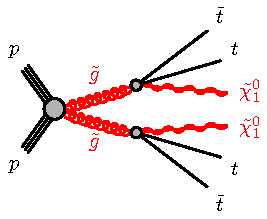
\includegraphics[width=0.35\textwidth]{figures/strong_prod/diagrams/gogo-ttttN1N1.pdf}\label{fig:diagram_Gtt}}
\subfigure[]{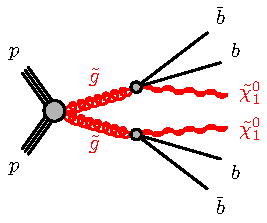
\includegraphics[width=0.35\textwidth]{figures/strong_prod/diagrams/gogo-bbbbN1N1.pdf}\label{fig:diagram_Gbb}}
\caption{The simplified models used for the optimization of the analysis. \subref{fig:diagram_Gtt} Gtt model. \subref{fig:diagram_Gbb} Gbb model.
}\label{fig:strong_diagram}
\end{figure*}

In the Gtt and Gbb models, since the \stop and \sbottom are assumed to have very high mass, the only parameters are the mass and production cross section of the gluino, and the mass of the \gls{lsp}. While the Gtt and Gbb models are used both to optimize and interpret the analysis, a further interpretation is provided also in terms of a slightly more complicated model. If we allow also the lightest chargino (\chinoonepm) be kinematically accessible, another decay chain opens, where the virtual stop or sbottom decays to a \chinoonepm:
$\stop \to \bar{b} \chinoonem$ and 
$\sbottom \to t \chinoonem$.
The charge-conjugate processes are also possible, and in both cases the overall decay chain of the gluino leads to $\gluino \to t b \chinoonem$, which we refer to as Gtb model.
The model used to reinterpret this analysis assumes the decay $\chinoonepm \to \ninoone W^{\pm}$, where the $W$ boson can be off-shell if the mass difference between the \chinoonepm and the \ninoone is not large enough to produce an on-shell $W$ boson. 
This mass difference becomes a further parameter of the model, and in this analysis we assume that the \chinoonepm and the \ninoone 
are almost degenerate (in the \gls{mc} simulation, they are generated with a mass difference of 2 GeV); in this case the $W$ boson is virtual and results into soft fermions, which most of the time are not reconstructed. This small mass difference is often verified in models where the \chinoonepm and the \ninoone are part of an approximate $SU(2)$ multiplet, and setting it to a fixed value allows reducing the number of parameters of the model. 
This analysis provides an interpretation of the result in terms of the \gls{br} of the gluino into the Gtt, Gbb and Gtb models. 
A schematic diagram of the possible decay chains in this mixed-\gls{br} interpretation, in addition to the ones shown in Figure \ref{fig:strong_diagram}, is shown in Figure \ref{fig:strong_diagram_br}.

\begin{figure*}[h]
\centering 
\subfigure[]{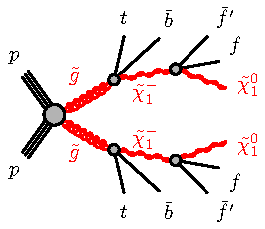
\includegraphics[width=0.35\textwidth]{figures/strong_prod/diagrams/gogo-tbfftbffN1N1.pdf}\label{fig:diagram_strong_tbtb}}
\subfigure[]{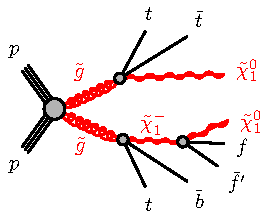
\includegraphics[width=0.35\textwidth]{figures/strong_prod/diagrams/gogo-tttbffN1N1.pdf}\label{fig:diagram_strong_tttb}}\\
\subfigure[]{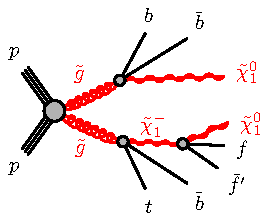
\includegraphics[width=0.35\textwidth]{figures/strong_prod/diagrams/gogo-bbtbffN1N1.pdf}\label{fig:diagram_strong_bbtb}}
\subfigure[]{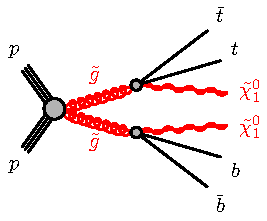
\includegraphics[width=0.35\textwidth]{figures/strong_prod/diagrams/gogo-ttbbN1N1.pdf}\label{fig:diagram_strong_ttbb}}
\caption{Simplified models used in the reinterpretation of the analysis. \subref{fig:diagram_strong_tbtb} Both gluinos have the following decay chain: $\gluino \to t \bar{b} \chinoonem$ with $\chinoonem \to f\bar{f}' \ninoone$. \subref{fig:diagram_strong_tttb} One gluino decays as in \subref{fig:diagram_strong_tbtb} and the other as $\gluino \to t\bar{t}\ninoone$. \subref{fig:diagram_strong_bbtb} One gluino decays as in \subref{fig:diagram_strong_tbtb} and the other as $\gluino \to b\bar{b}\ninoone$. \subref{fig:diagram_strong_ttbb} One gluino decays as $\gluino \to t\bar{t}\ninoone$ and the other as $\gluino \to b\bar{b}\ninoone$.  %The charge conjugate processes are implied.
%The fermions originating from the $\chinoonepm$ decay are typically soft because the mass difference  between the $\chinoonepm$ and the $\ninoone$ is fixed to 2 GeV. 
}\label{fig:strong_diagram_br}
\end{figure*}


These gluino decay chains that lead to final states rich in heavy-flavour quarks are dominant in \gls{susy} models where the squarks 
from the first two generations are significantly heavier than stop and sbottom, or also in cases when the \ninoone is dominated by the higgsino component. 

\subsection{Signal cross-section}
\label{sec:strong:signalxsec}

The cross section for the production of a gluino pair at \cmtre TeV, considering all the other \gls{susy} particles decoupled, is shown in Figure 
\ref{fig:strong:xsec}. This computation is at \gls{nlo} accuracy in the strong coupling constant, adding the resummation of soft emissions at \gls{nll}.
To compute the nominal cross-section and its uncertainty, the envelope of the predictions obtained with different choices of factorization scale, 
renormalization scale and \gls{pdf} set is built; the nominal cross-section is defined as the midpoint of this envelope, and the uncertainty as 
half of the envelope width, as described in Ref. \cite{Borschensky:2014cia}.


\begin{figure*}[h]
\centering 
%\subfigure[]{
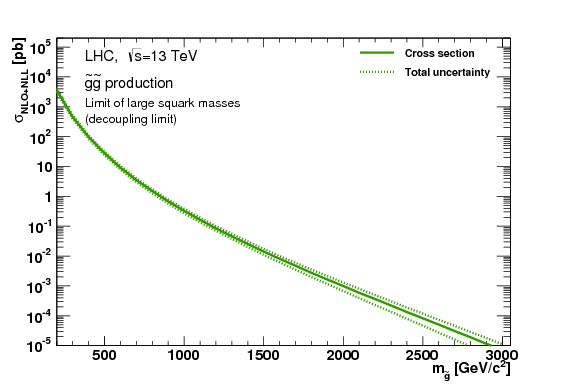
\includegraphics[width=0.70\textwidth]{figures/strong_prod/diagrams/XSectionPlots_13TeV_Gluino_decouplingLimit_xsec_gg_200_3050}
%\label{fig:}}
\caption{NLO+NLL gluino pair production cross section with squarks decoupled as a function of mass at \cmtre TeV. Figure from Ref. \cite{Borschensky:2014cia}.
}\label{fig:strong:xsec}
\end{figure*}

%\section{Previous limits}


\section{Discriminating variables}
\label{sec:strong:sigbkg}

Most of the kinematic variables used in this analysis to discriminate between signal and background 
are in common with the Higgsino search and have already been discussed in Section \ref{sec:common_variables}.
Two additional variables, used only in this analysis, are defined in this section.

\subsubsection*{Total jet mass}

The total jet mass is the sum of the masses of the four leading reclustered jets in the event:

\begin{equation}
\mjsum = \sum_{i \leq 4} m_{J,i} \; .
\end{equation}

\noindent This variable is particularly useful in the case of boosted Gtt signals, where the four top quarks are produced with high momentum and can be reconstructed as reclustered jets with high mass. 

\subsubsection*{ISR jet}

In the case of Gbb models, when the mass of the neutralino is close to the mass of the gluino the neutralino is produced almost at rest and the event does not have a sizable \met; this reduces the sensitivity of the analysis to these cases. 
For these signal models, a sizable value of \met can be present in events where the gluino system is recoiling against a hard jet from \gls{isr}; if we assume that the \gls{isr} jet is the most energetic jet in the event, there will be an angular separation between this jet and \met larger than the average. The variable \dphilead, defined as:

\begin{equation}
\dphilead = |{\Delta}{\phi}(j_1, \met)| \; ,
\end{equation}

\noindent helps therefore in selecting signal events where the \met derives from a neutralino boosted by an \gls{isr} jet. 


The variables defined above, together with the ones defined in Section \ref{sec:common_variables},
allow to 
identify a region of the phase space that is enriched in signal events. 
After selecting events with high \met ($> 200$ GeV), at least four signal jets and at least three $b$-tagged jets, events are
divided into the 0-lepton category, which requires a lepton veto and also \dphimin $>0.4$, and the 1-lepton category, 
with at least one signal lepton.
Figures \ref{fig:strong:sig:bjets_n} to \ref{fig:strong:sig:met} show the distribution of some important kinematic variables for 
the sum of the \gls{sm} backgrounds and for selected signal samples. 

From Figure \ref{fig:strong:sig:bjets_n} it is possible to see how signal events have in general higher number of 
$b$-tagged jets than background events; despite this, this variable alone is not sufficient to reduce the number of 
background events enough to be sensitive to the signal.

Figure \ref{fig:strong:sig:jets_n} shows the distribution of the number of signal jets. 
In this case, the result of the comparison between the shape of the distribution for signal and for backgrounds depends heavily 
on the specific signal considered. In particular, Gbb signal models tend to have a lower number of jets than Gtt models; 
this is expected, since in Gtt models the decay of the top quark to a $b$-quark and a $W$ boson can lead to up to 12 jets originating from the 
hard scattering process, while only four of such jets are present in Gbb signals. 
Furthermore, Gtt events in the 0-lepton channel have more jets than Gttt-events in the 1-lepton channel, since the leptonic decays of the $W$ boson 
reduce the amount of hadronic activity in the final state. 
It can be noted that while in \gls{sm} simulations all-hadronic \ttbar events do not enter our analysis regions because of the lack of real \met,  there are signal events where all the top quarks decay hadronically, since the \met is provided by the neutralino. 

A key variable in the suppression of the \ttbar background is \mtb, whose distribution is shown in Figure \ref{fig:strong:sig:mTb_min}.
The kinematic endpoint that characterizes \ttbar events is not present for signal events, which tend to have a more uniform distribution.
Despite not having a kinematic endpoint, not all signals have a \mtb distribution that reaches high values: this is more likely for 
signals with a large splitting between the gluino and the neutralino masses, which leads to the decay products being boosted.

The \meff distribution for signal and background events is shown in Figure \ref{fig:strong:sig:meff_incl}. 
In this case it is possible to observe how signal models with a low neutralino mass (and therefore a large mass splitting)
this variable can be extremely helpful in identifying the presence of signal. 
In contrast, \meff does not offer a large discriminating power for signals that originate from less energetic final states, as it is the 
case for the region of the parameter space where the mass of the neutralino approaches the mass of the gluino.
A similar argument can be made for \mjsum and \met, shown in Figures \ref{fig:strong:sig:MJSum_rc_r08pt10} and \ref{fig:strong:sig:met} respectively. 


\begin{figure*}[htbp]
\centering 
\subfigure[]{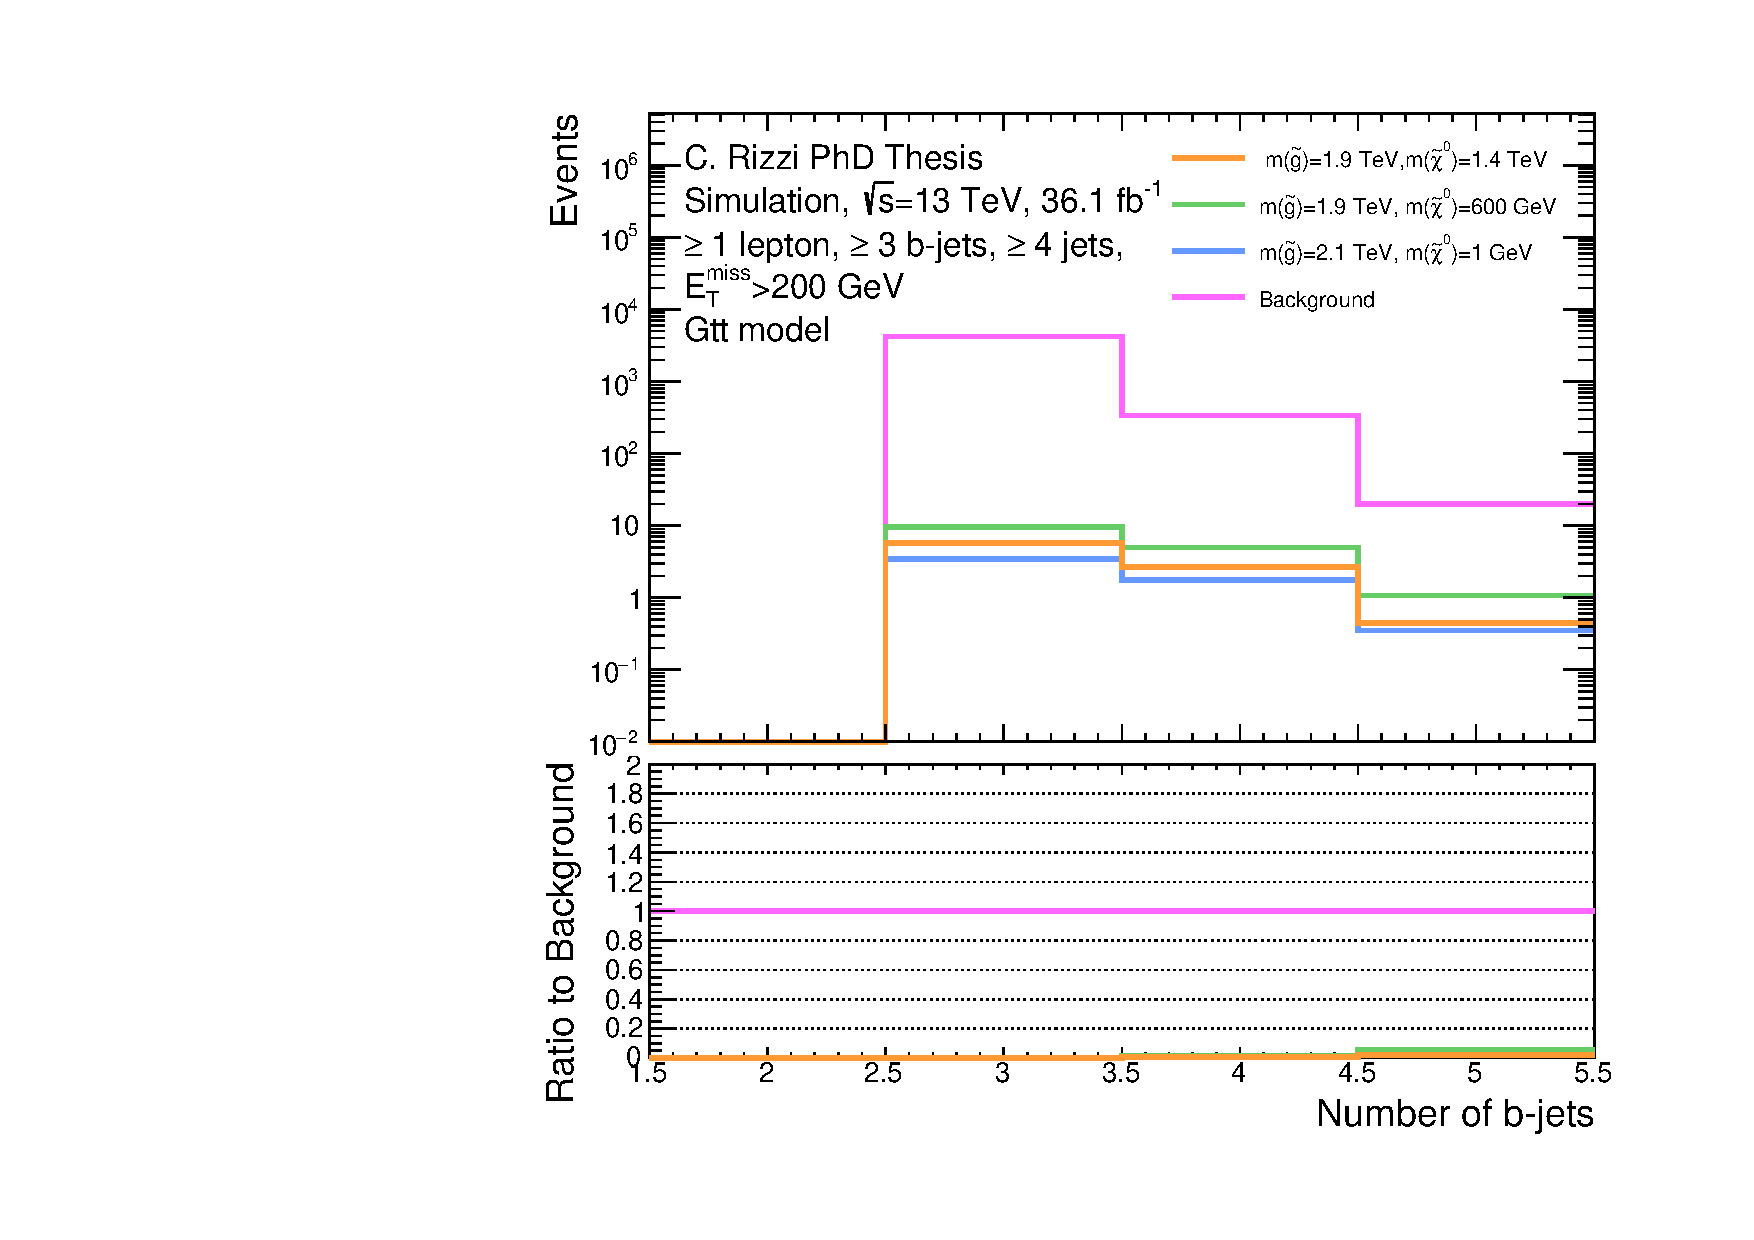
\includegraphics[width=0.325\textwidth]{figures/strong_prod/sig_bkg_strong/1L_3b/Gtt_compare_bjets_n.pdf}\label{fig:strong:sig:bjets_nA}}
\subfigure[]{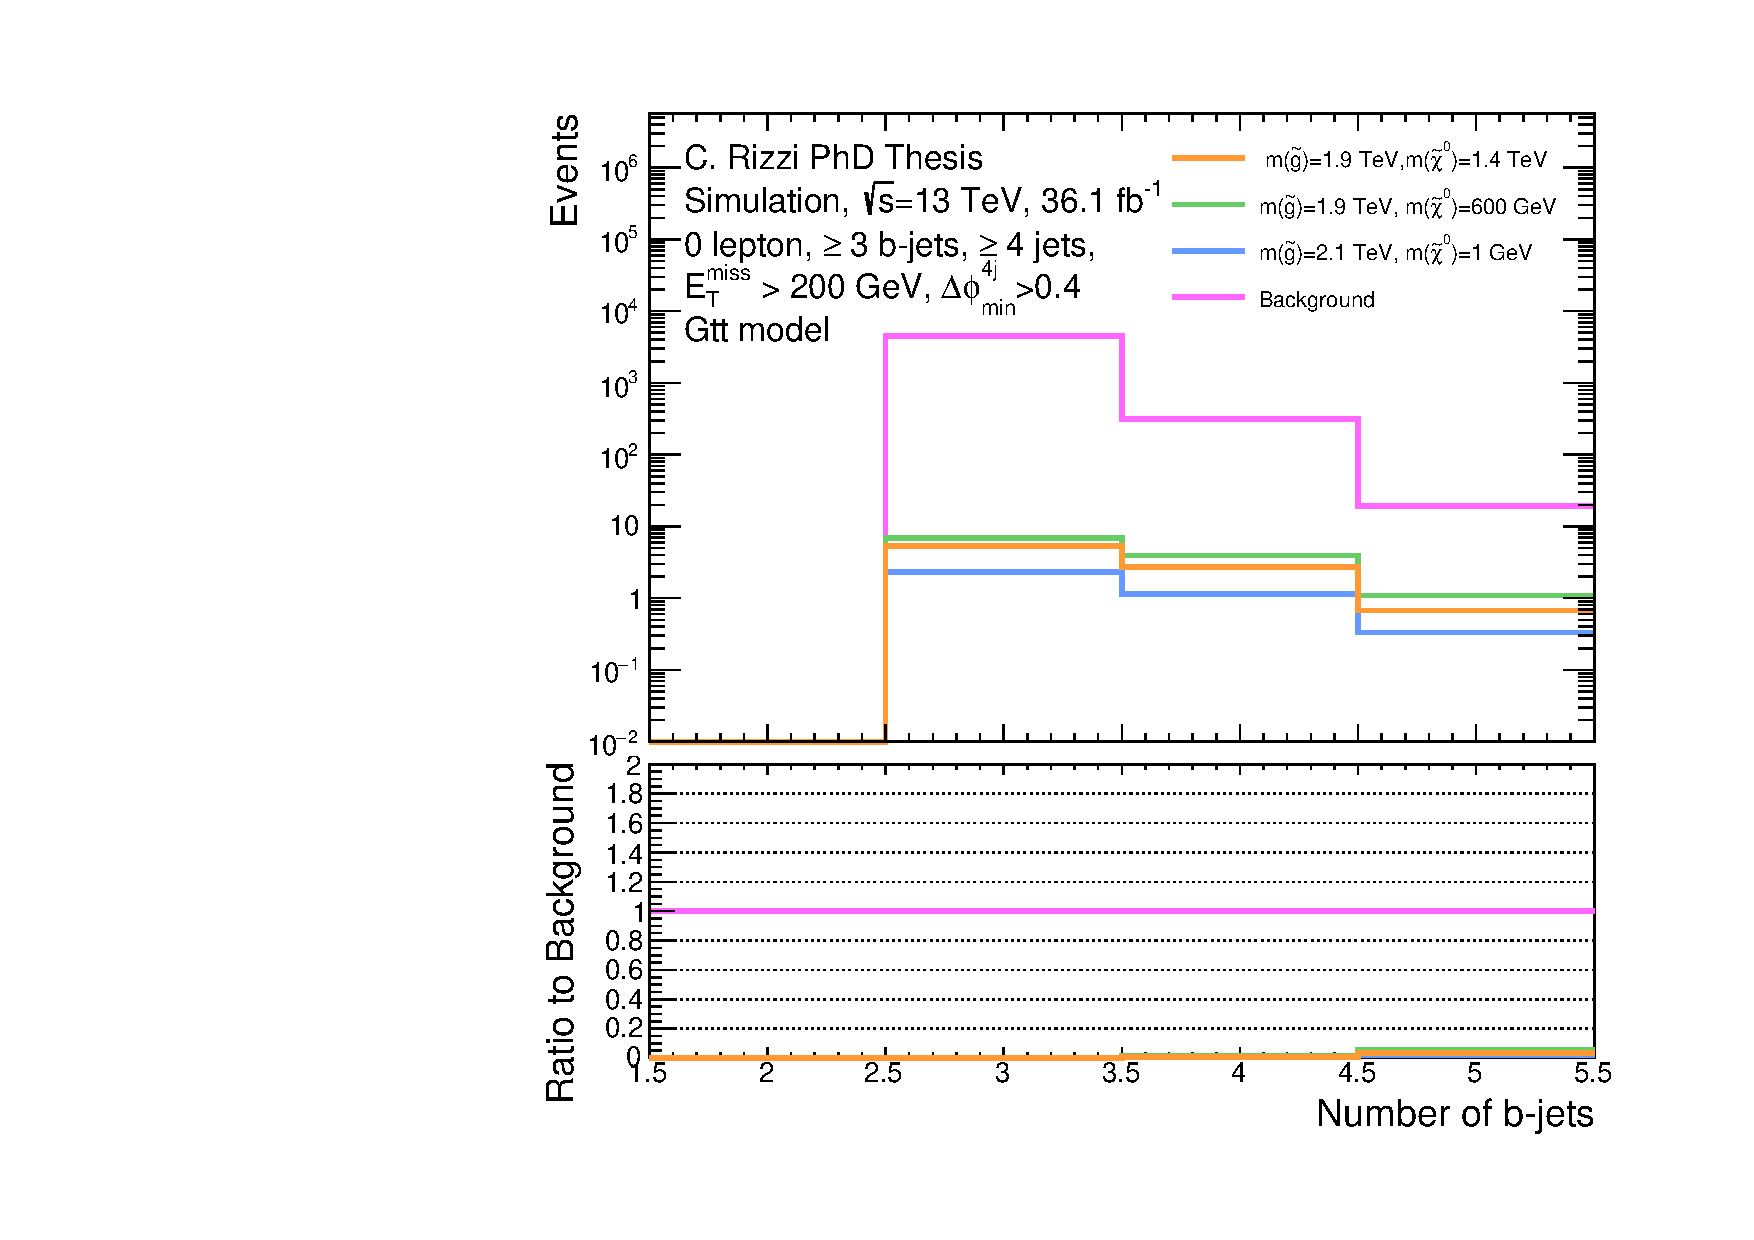
\includegraphics[width=0.325\textwidth]{figures/strong_prod/sig_bkg_strong/0L_3b/Gtt_compare_bjets_n.pdf}\label{fig:strong:sig:bjets_nB}}
\subfigure[]{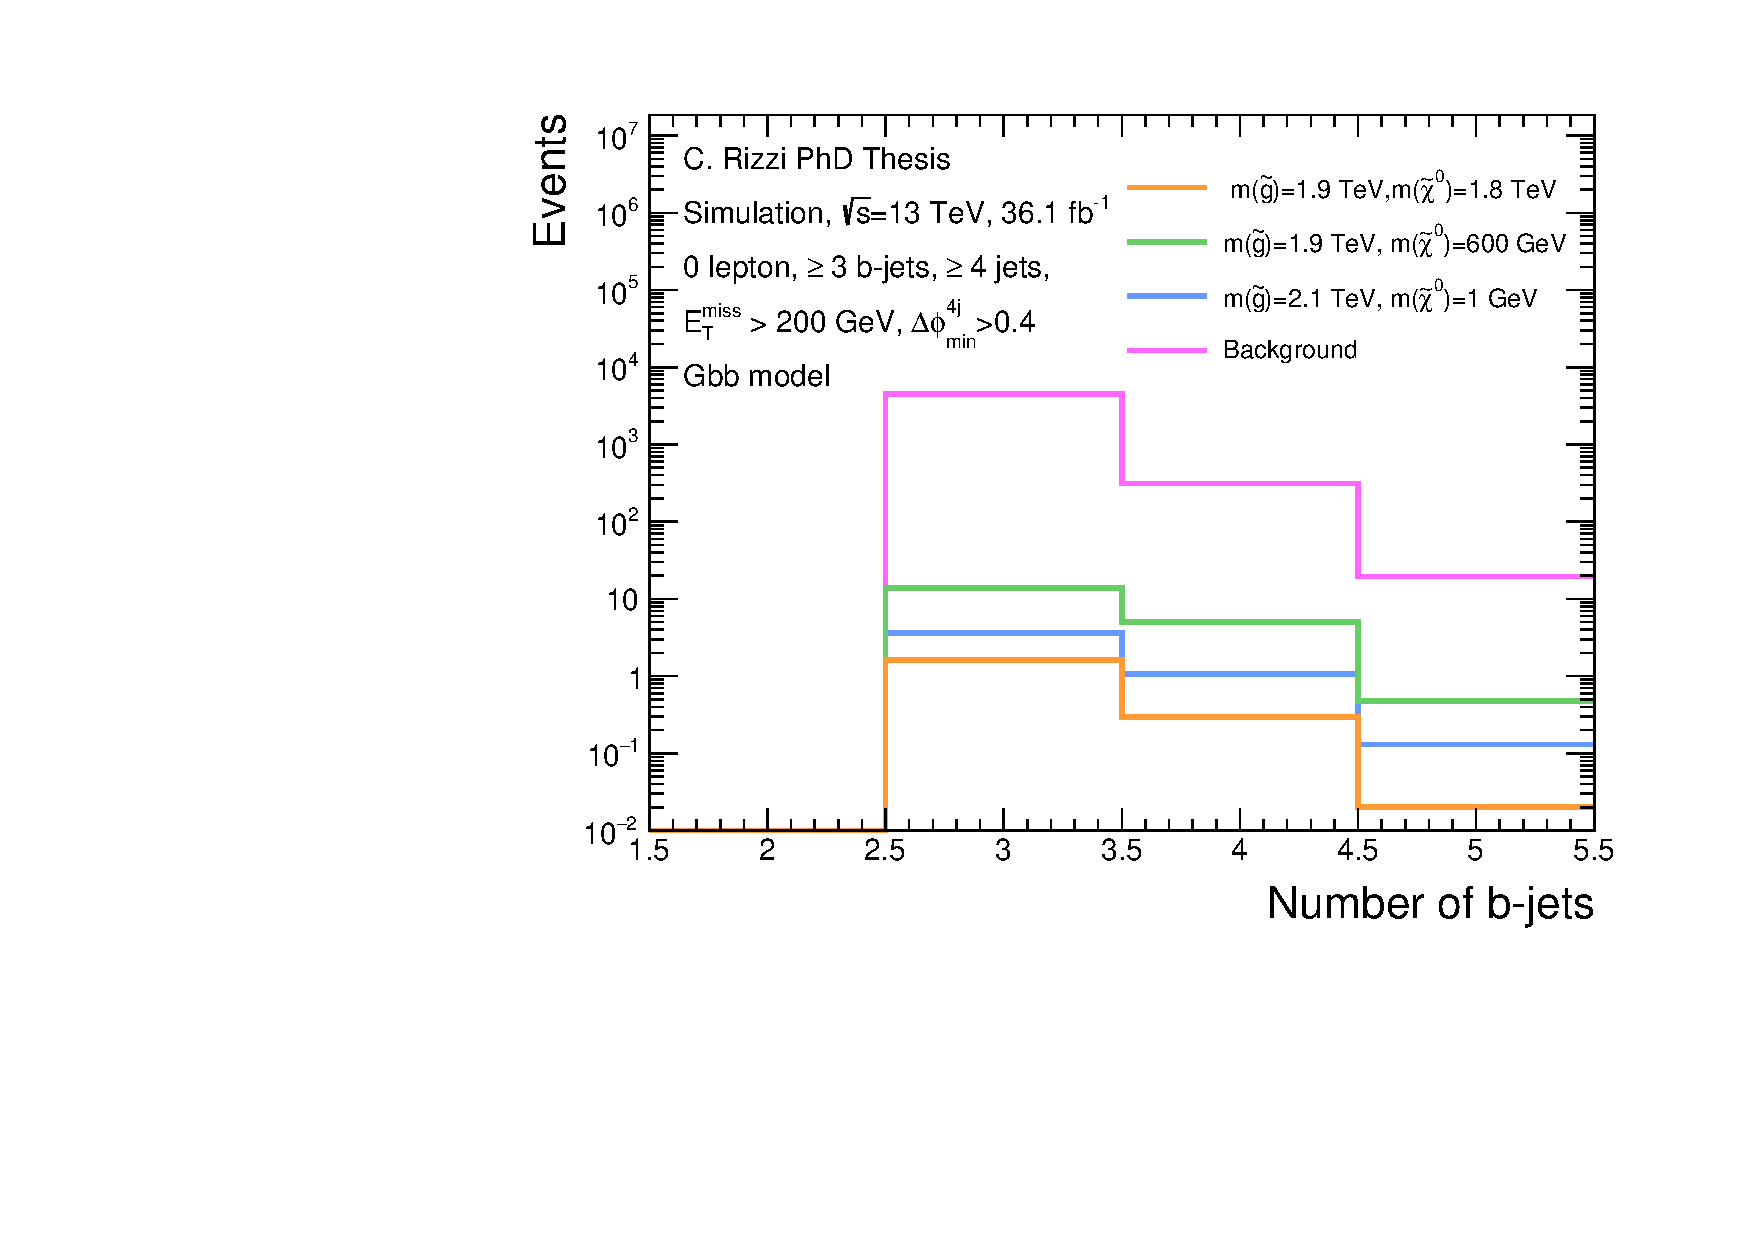
\includegraphics[width=0.325\textwidth]{figures/strong_prod/sig_bkg_strong/0L_3b/Gbb_compare_bjets_n.pdf}\label{fig:strong:sig:bjets_nC}}
\caption{Distribution of number of $b$-tagged jets in background events and in \subref{fig:strong:sig:bjets_nA} Gtt signals in a 1-lepton selection,
\subref{fig:strong:sig:bjets_nB} Gtt signals in a 0-lepton selection and
\subref{fig:strong:sig:bjets_nC} Gbb signals in a 0-lepton selection.
}\label{fig:strong:sig:bjets_n}
\end{figure*}

\begin{figure*}[htbp]
\centering 
\subfigure[]{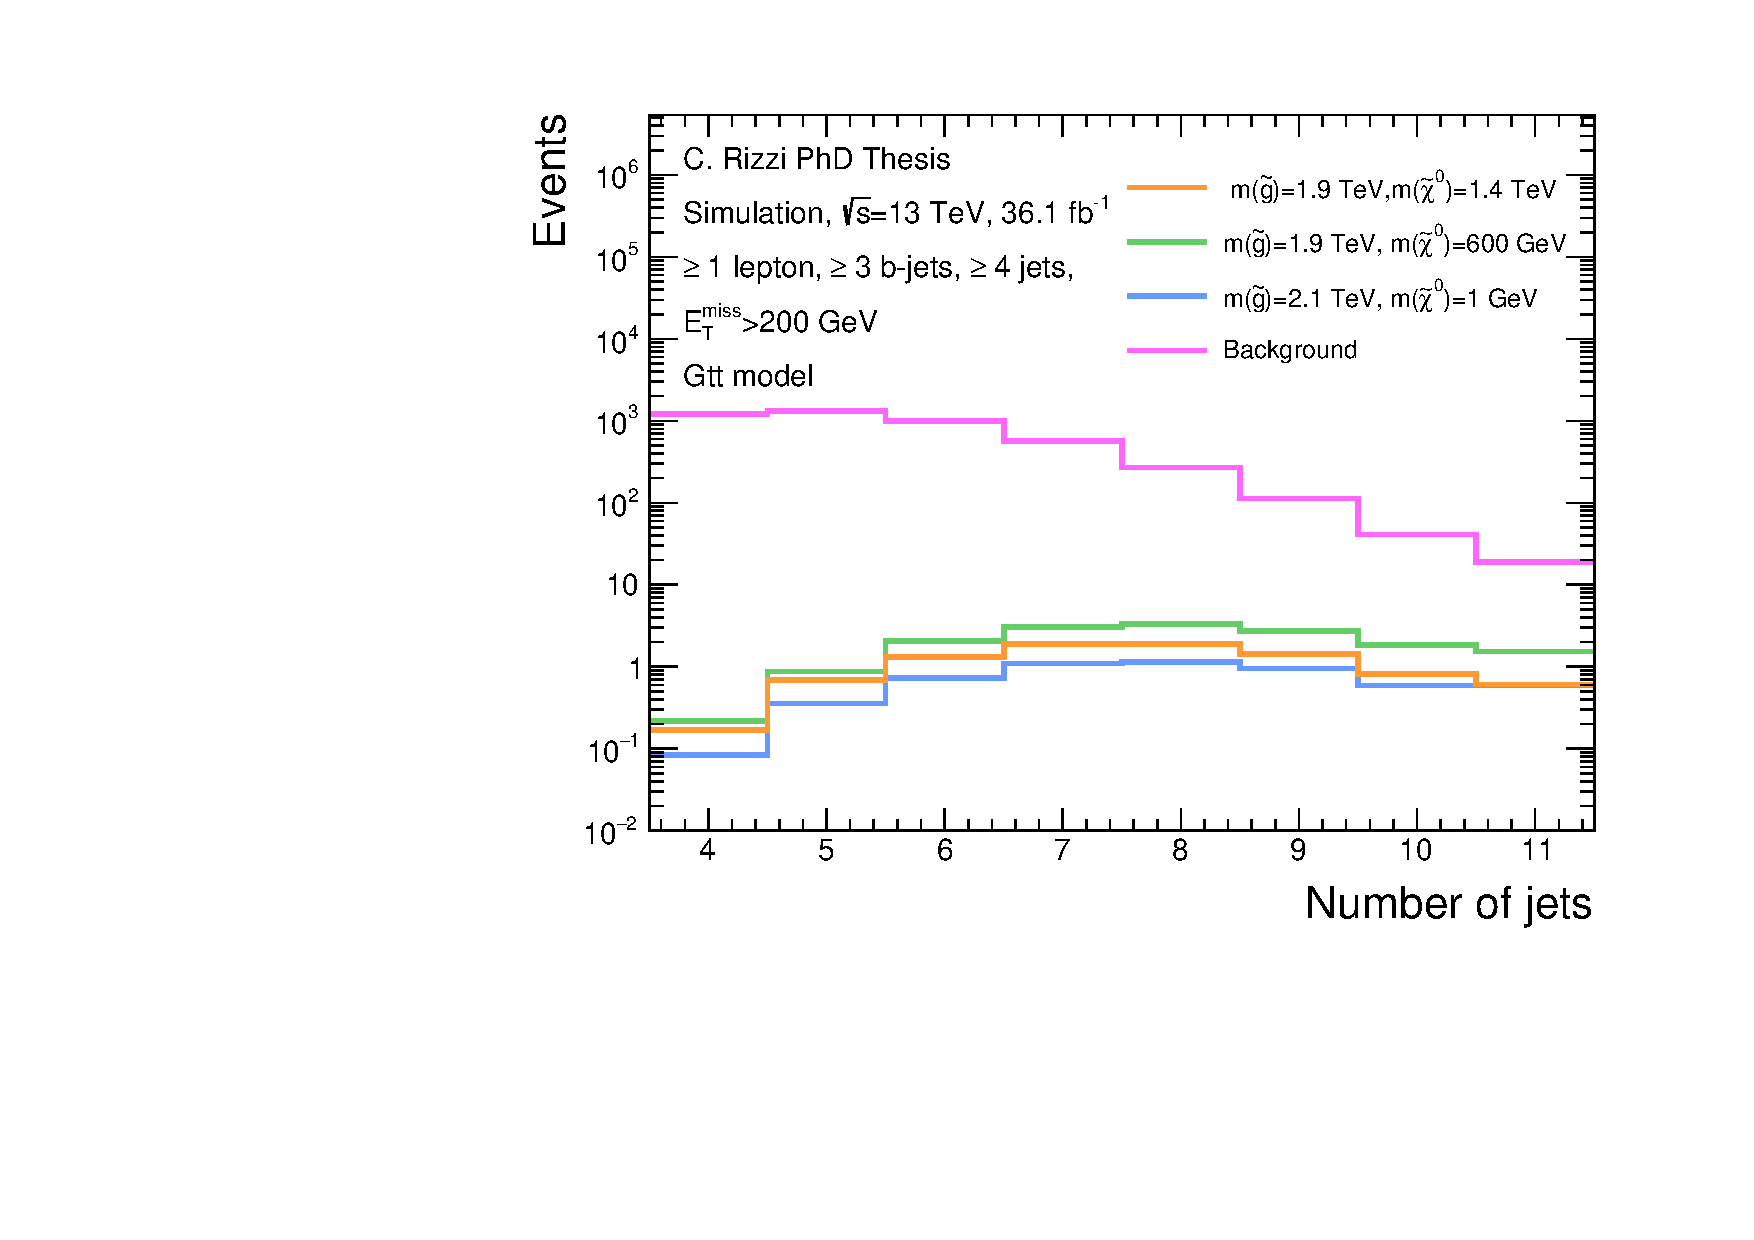
\includegraphics[width=0.325\textwidth]{figures/strong_prod/sig_bkg_strong/1L_3b/Gtt_compare_jets_n.pdf}\label{fig:strong:sig:jets_nA}}
\subfigure[]{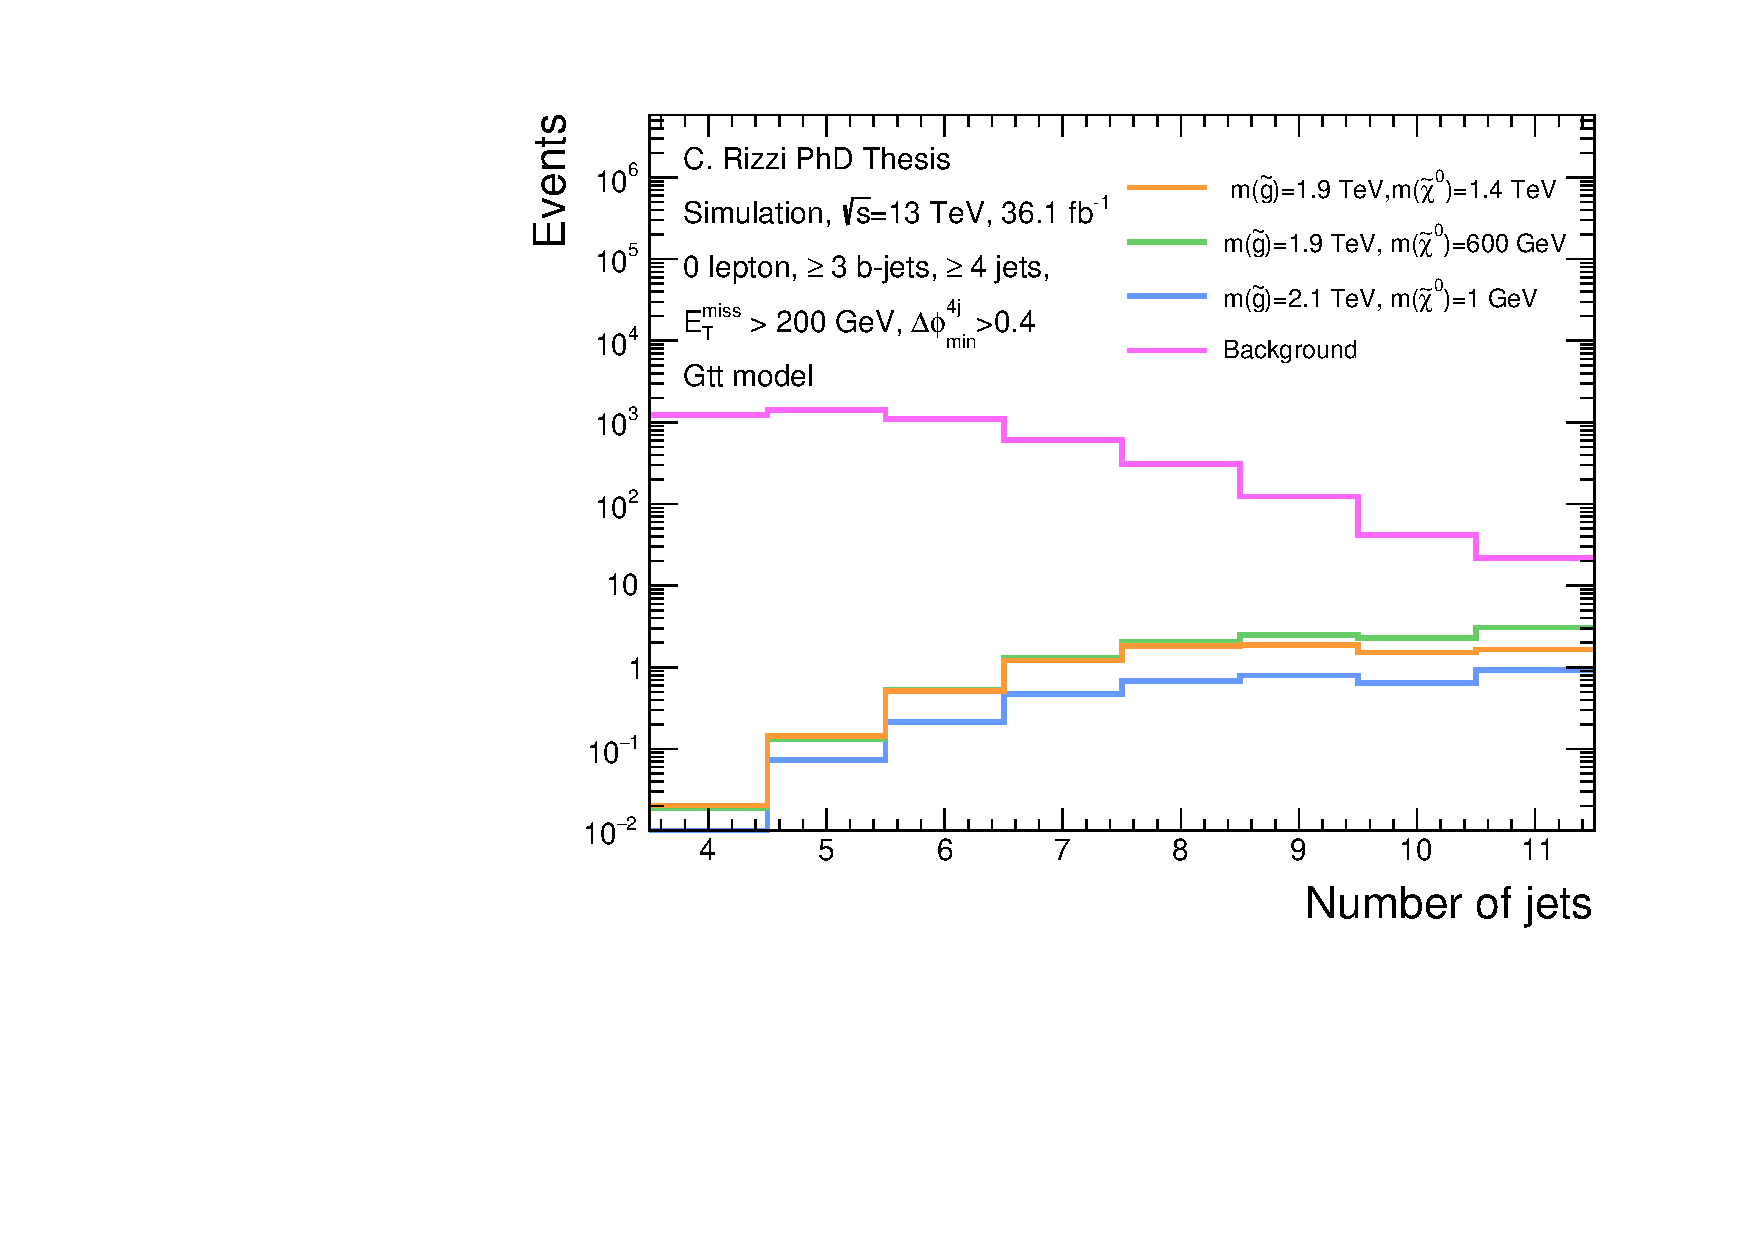
\includegraphics[width=0.325\textwidth]{figures/strong_prod/sig_bkg_strong/0L_3b/Gtt_compare_jets_n.pdf}\label{fig:strong:sig:jets_nB}}
\subfigure[]{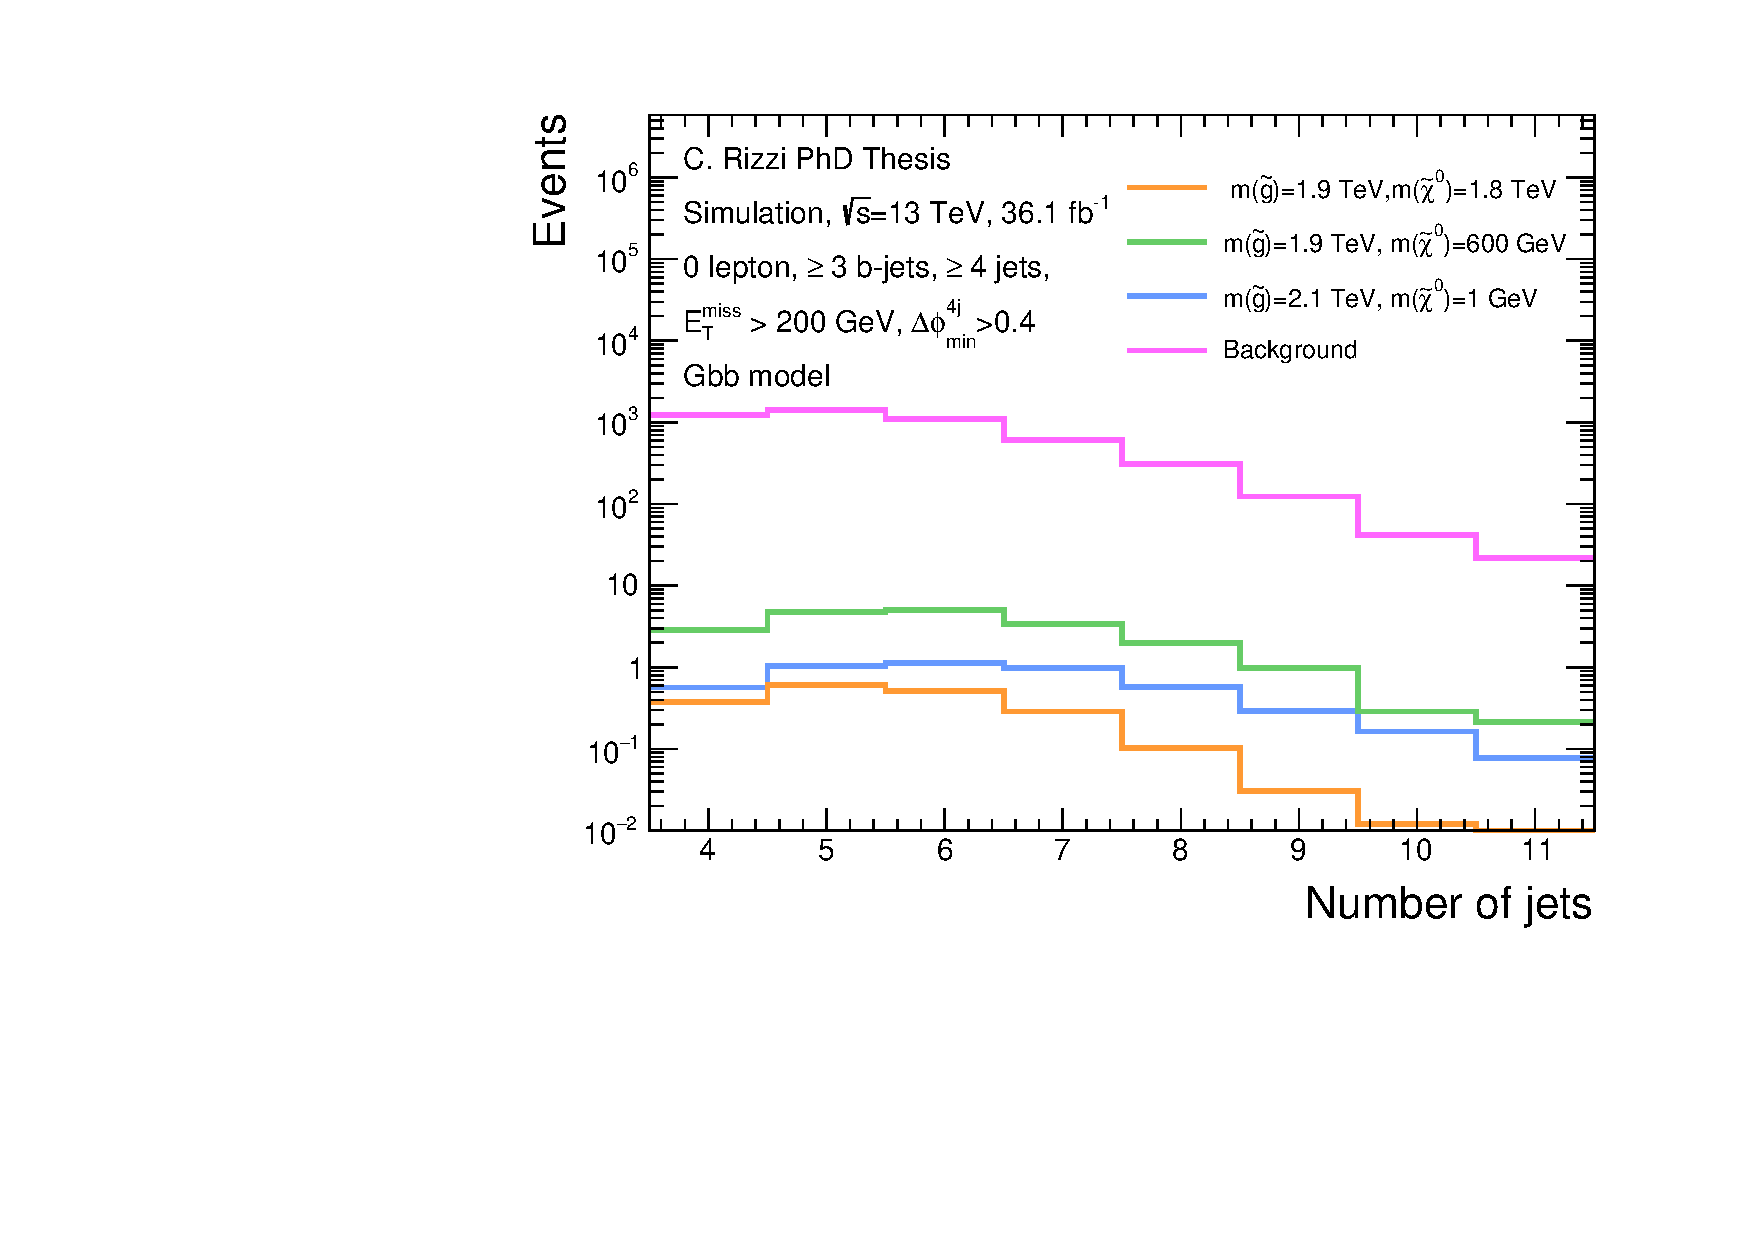
\includegraphics[width=0.325\textwidth]{figures/strong_prod/sig_bkg_strong/0L_3b/Gbb_compare_jets_n.pdf}\label{fig:strong:sig:jets_nC}}
\caption{Distribution of number of jets in background events and in \subref{fig:strong:sig:jets_nA} Gtt signals in a 1-lepton selection,
\subref{fig:strong:sig:jets_nB} Gtt signals in a 0-lepton selection and
\subref{fig:strong:sig:jets_nC} Gbb signals in a 0-lepton selection.
}\label{fig:strong:sig:jets_n}
\end{figure*}

\begin{figure*}[htbp]
\centering 
\subfigure[]{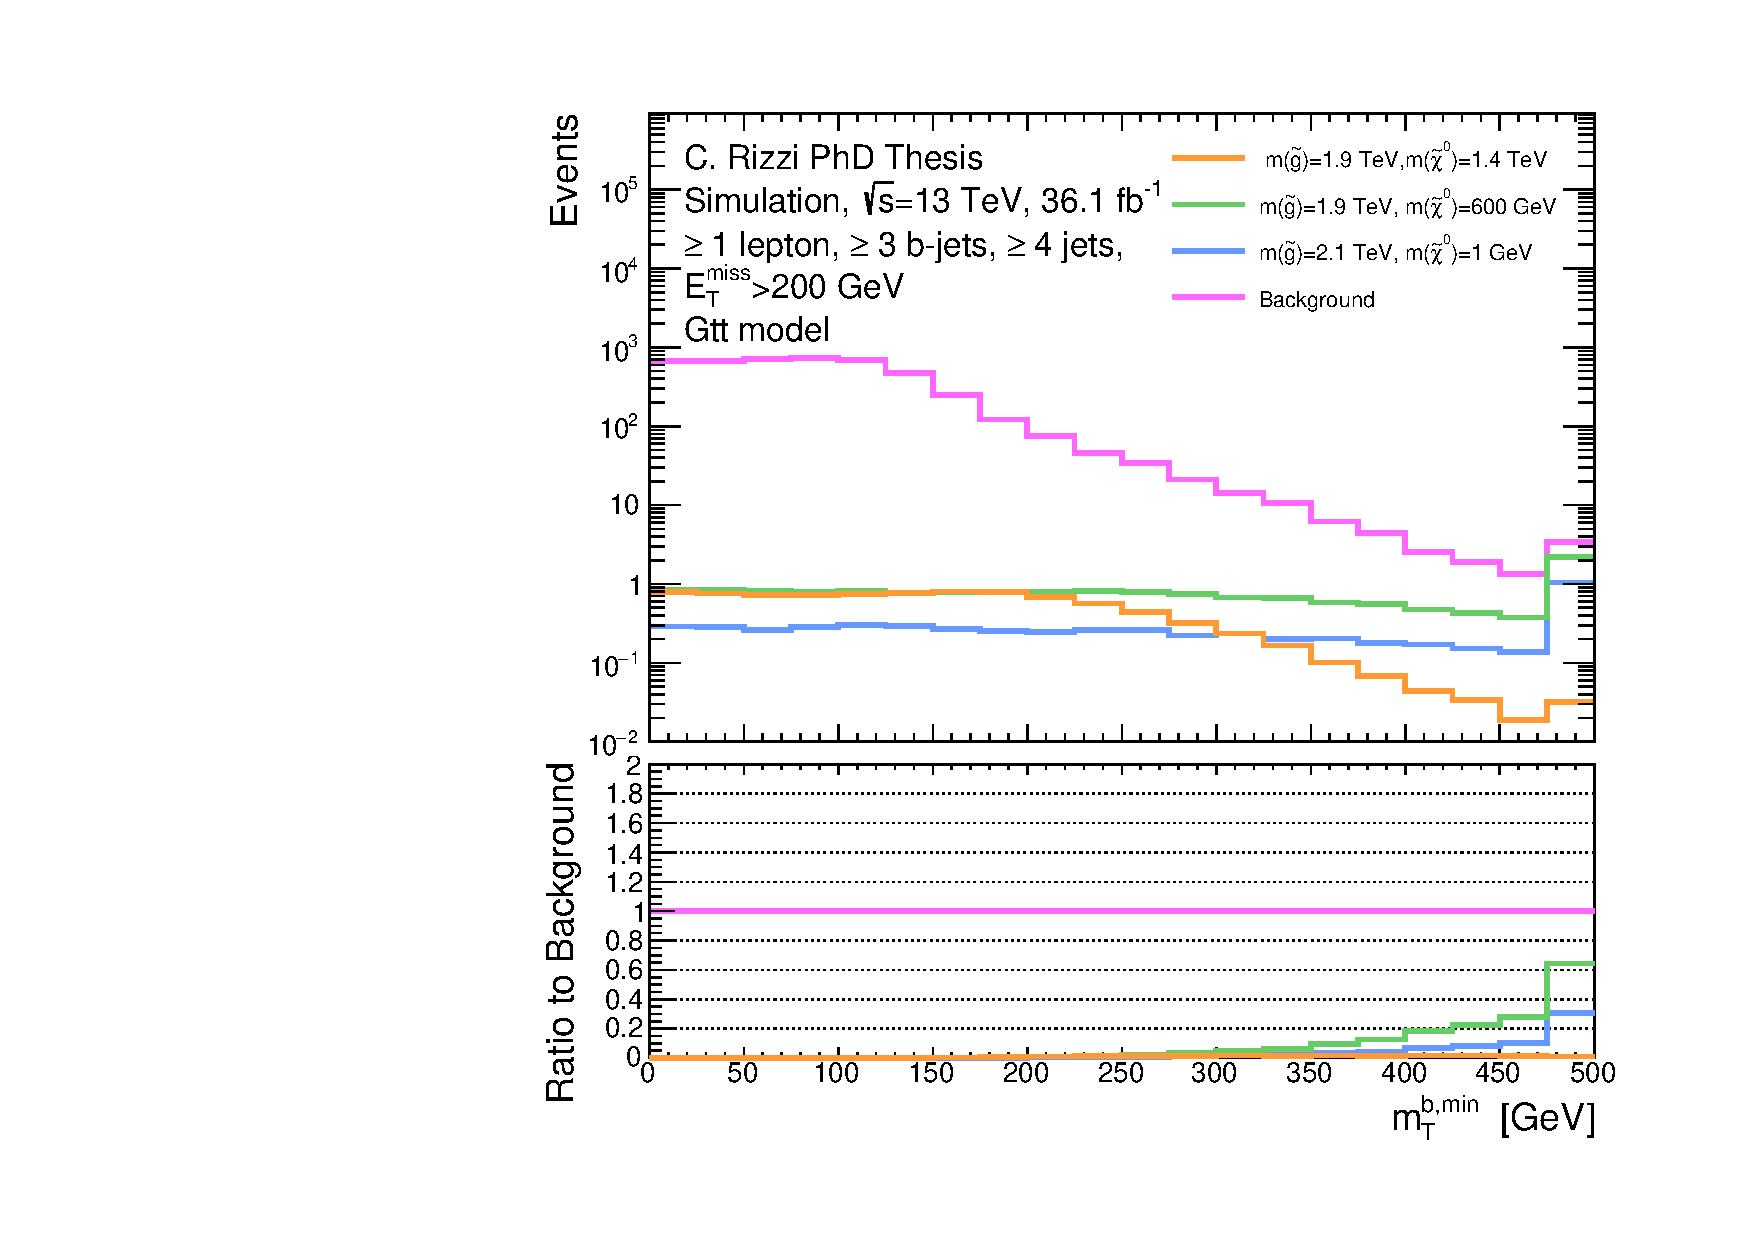
\includegraphics[width=0.325\textwidth]{figures/strong_prod/sig_bkg_strong/1L_3b/Gtt_compare_mTb_min.pdf}\label{fig:strong:sig:mTb_minA}}
\subfigure[]{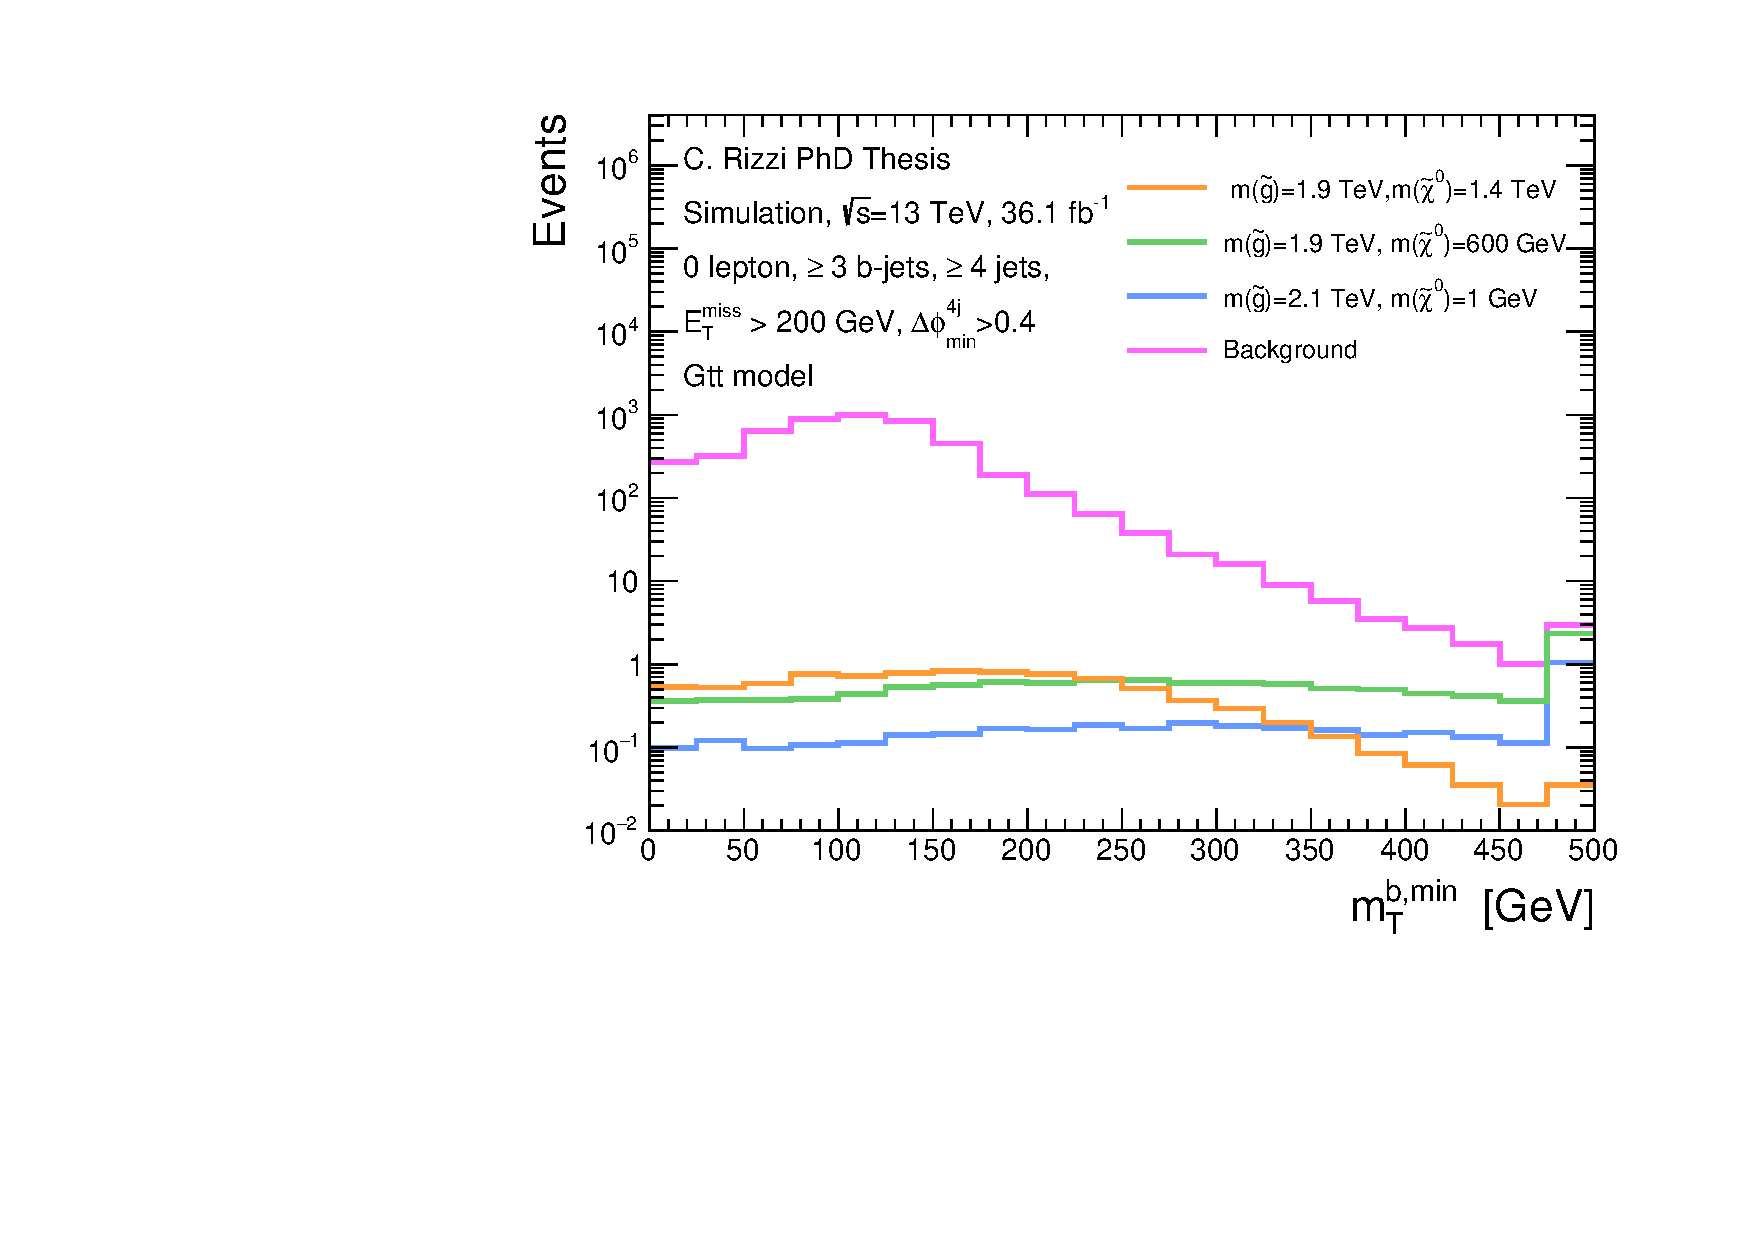
\includegraphics[width=0.325\textwidth]{figures/strong_prod/sig_bkg_strong/0L_3b/Gtt_compare_mTb_min.pdf}\label{fig:strong:sig:mTb_minB}}
\subfigure[]{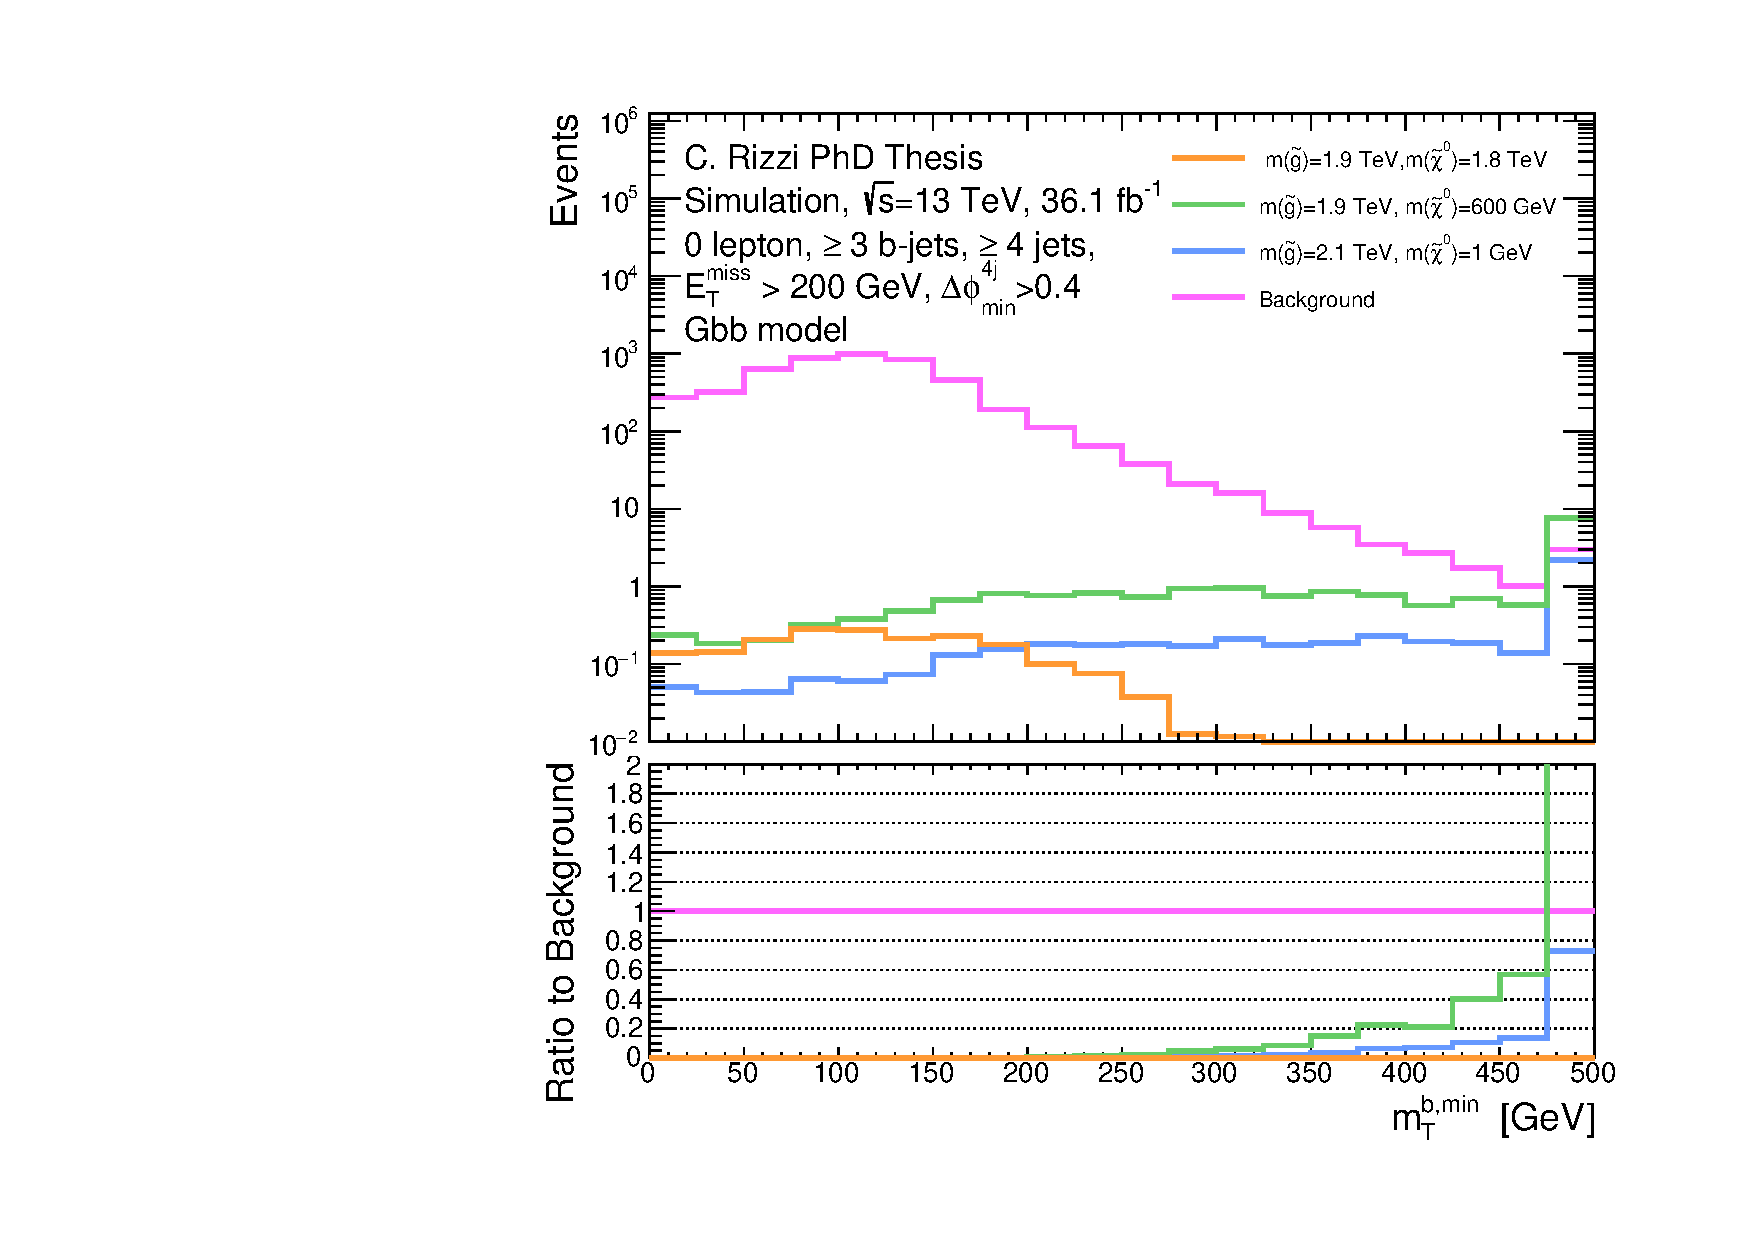
\includegraphics[width=0.325\textwidth]{figures/strong_prod/sig_bkg_strong/0L_3b/Gbb_compare_mTb_min.pdf}\label{fig:strong:sig:mTb_minC}}
\caption{Distribution of \mtb in  background events and in \subref{fig:strong:sig:mTb_minA} Gtt signals in a 1-lepton selection, 
\subref{fig:strong:sig:mTb_minB} Gtt signals in a 0-lepton selection and \subref{fig:strong:sig:mTb_minC} Gbb signals in a 0-lepton selection.
}\label{fig:strong:sig:mTb_min}
\end{figure*}

\begin{figure*}[htbp]
\centering 
\subfigure[]{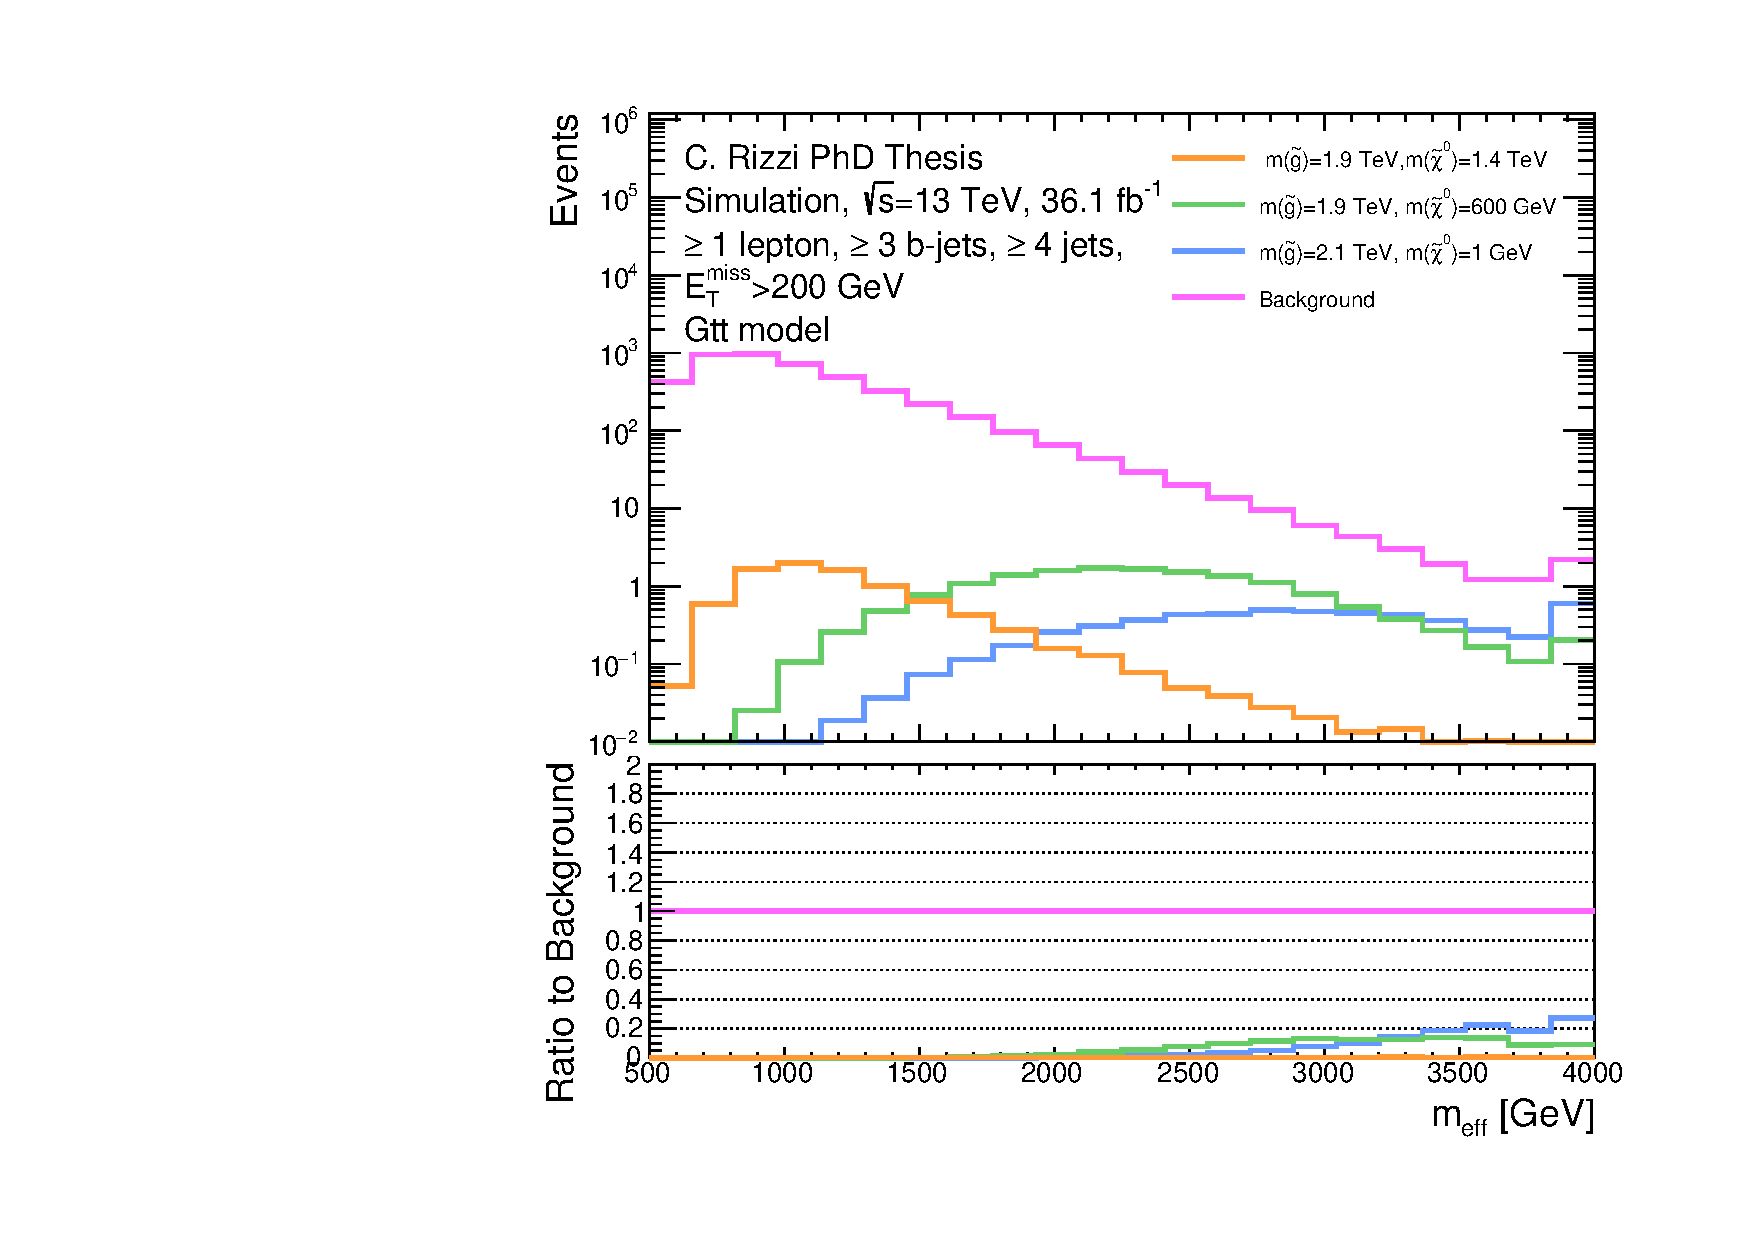
\includegraphics[width=0.325\textwidth]{figures/strong_prod/sig_bkg_strong/1L_3b/Gtt_compare_meff_incl.pdf}\label{fig:strong:sig:meff_inclA}}
\subfigure[]{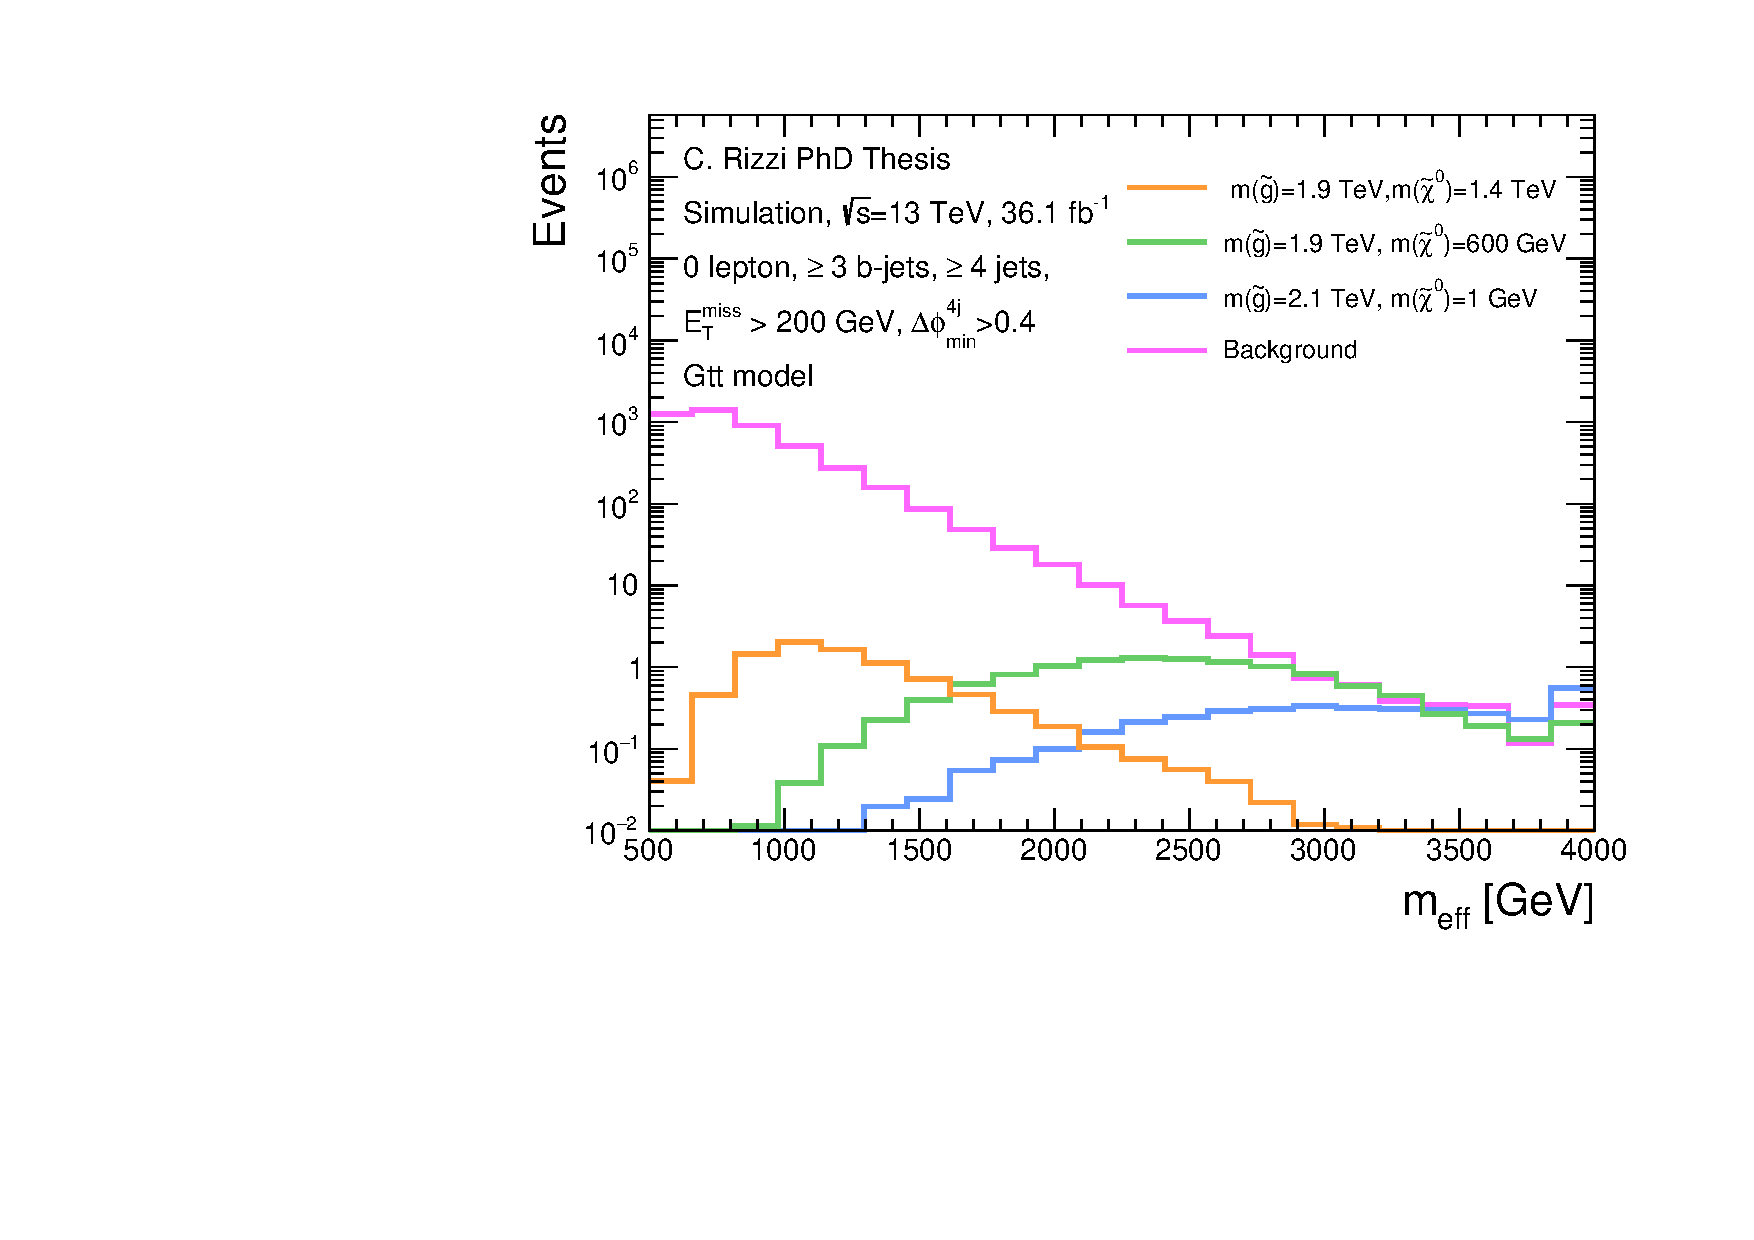
\includegraphics[width=0.325\textwidth]{figures/strong_prod/sig_bkg_strong/0L_3b/Gtt_compare_meff_incl.pdf}\label{fig:strong:sig:meff_inclB}}
\subfigure[]{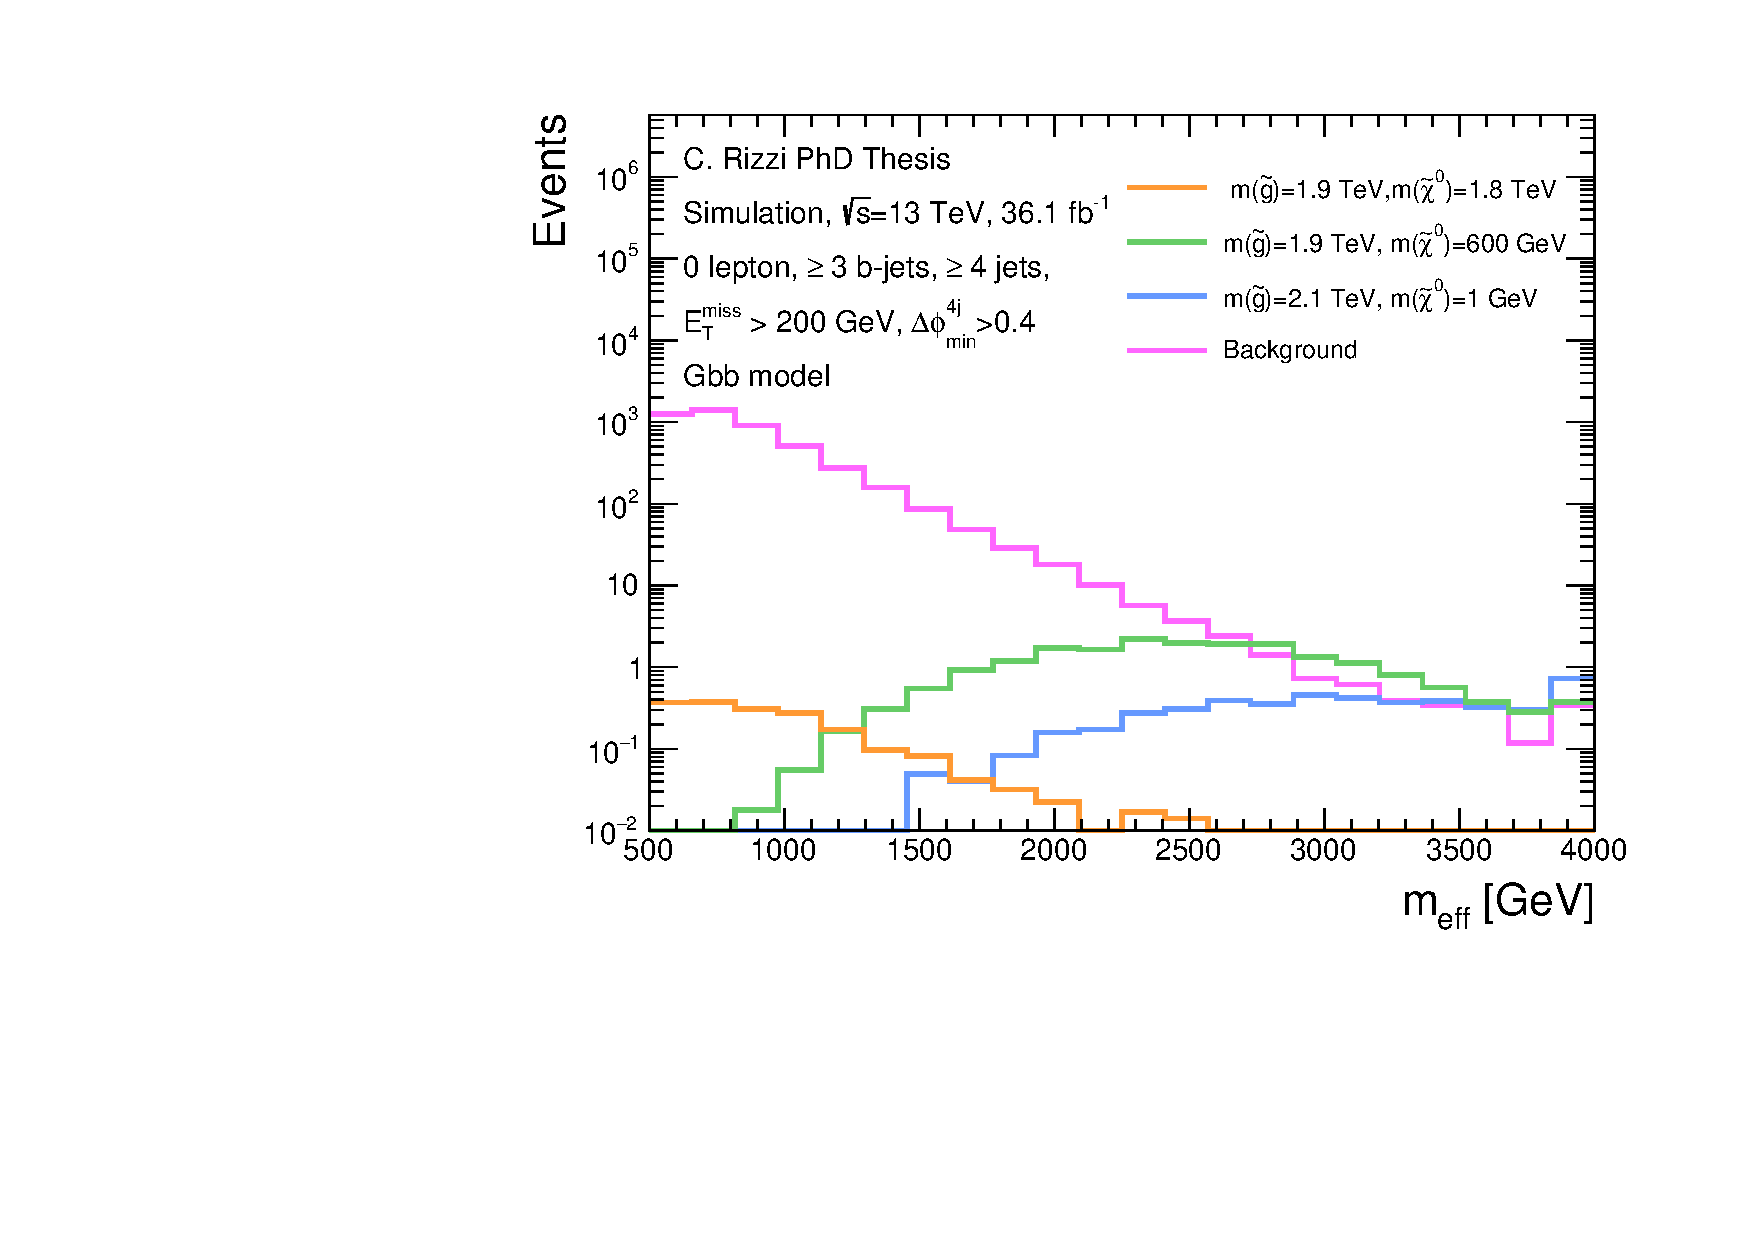
\includegraphics[width=0.325\textwidth]{figures/strong_prod/sig_bkg_strong/0L_3b/Gbb_compare_meff_incl.pdf}\label{fig:strong:sig:meff_inclC}}
\caption{Distribution of \meff in background events and in \subref{fig:strong:sig:meff_inclA} Gtt signals in a 1-lepton selection, \subref{fig:strong:sig:meff_inclB} Gtt signals in a 0-lepton selection and \subref{fig:strong:sig:meff_inclC} Gbb signals in a 0-lepton selection.
}\label{fig:strong:sig:meff_incl}
\end{figure*}


\begin{figure*}[htbp]
\centering 
\subfigure[]{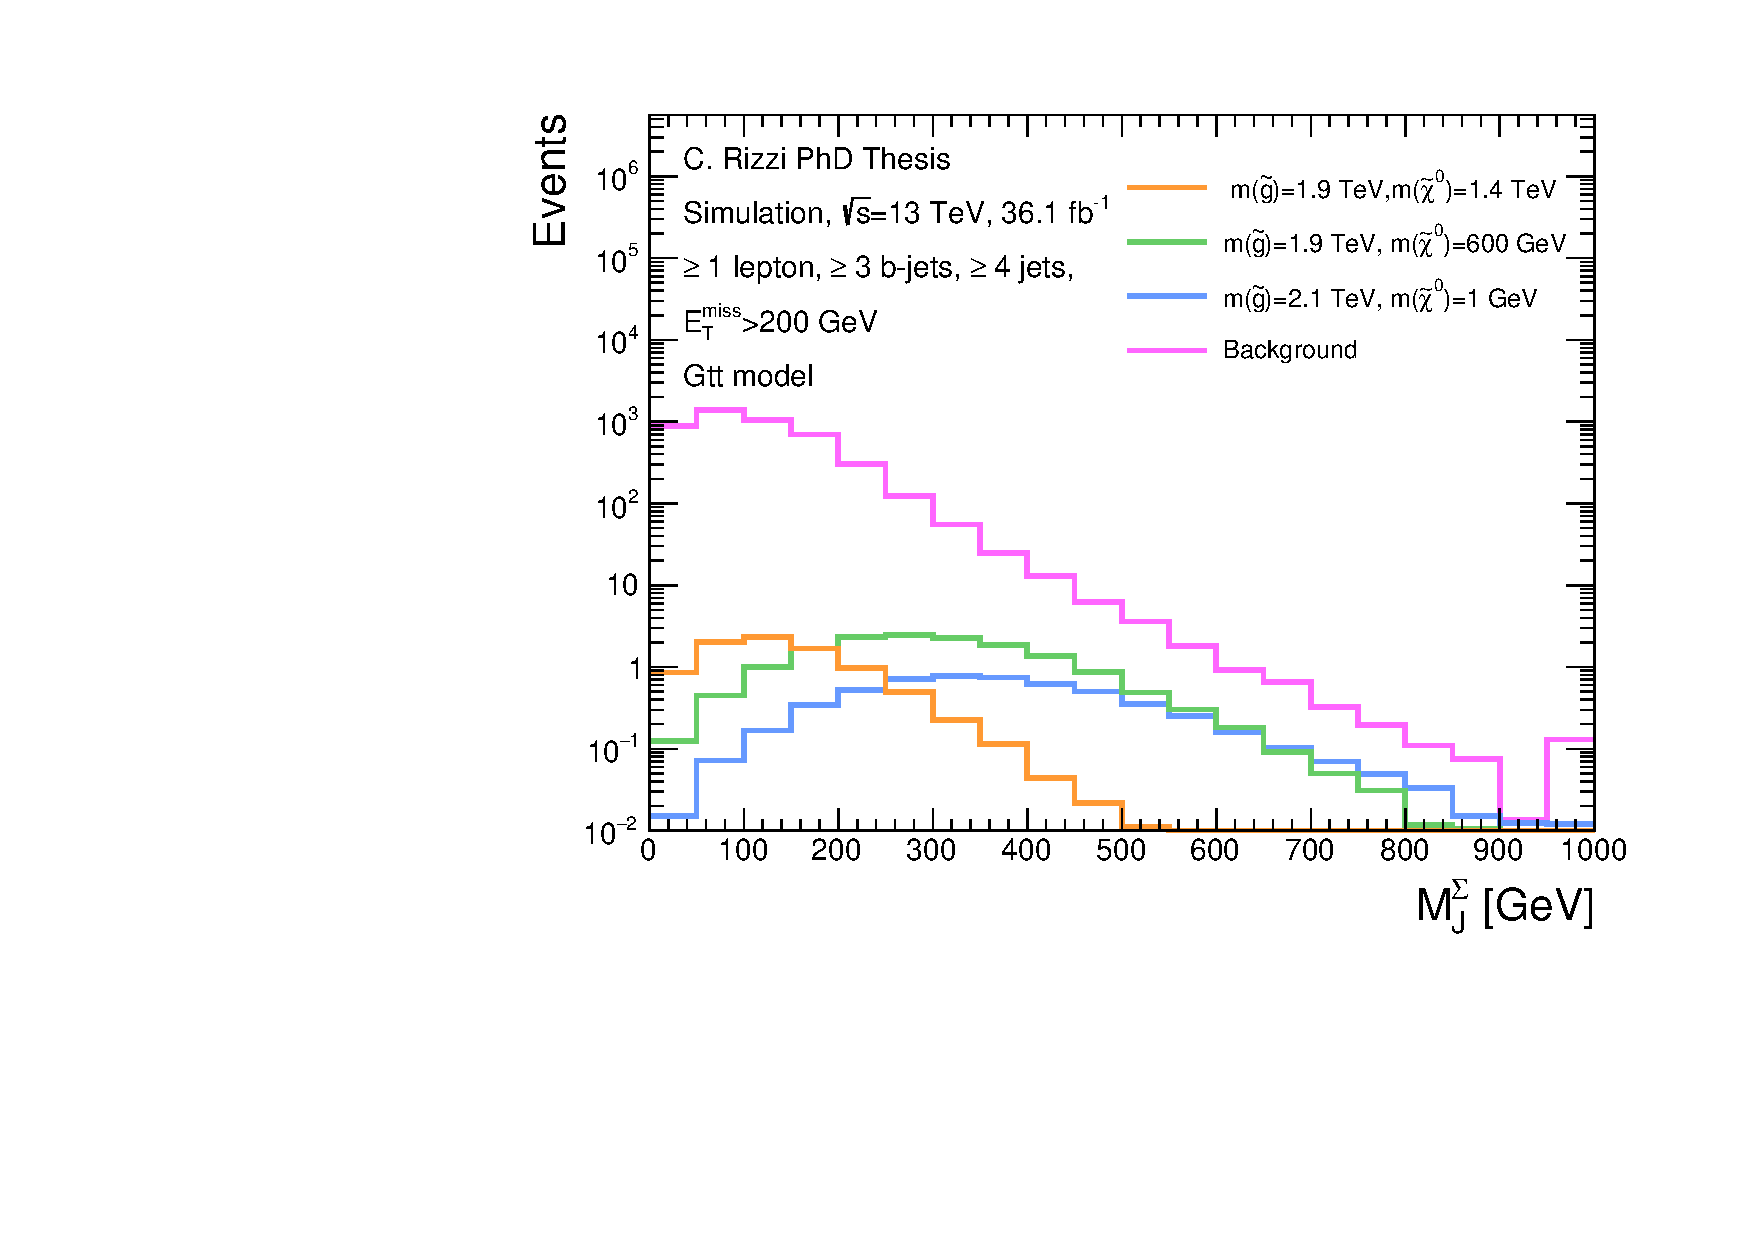
\includegraphics[width=0.325\textwidth]{figures/strong_prod/sig_bkg_strong/1L_3b/Gtt_compare_MJSum_rc_r08pt10.pdf}\label{fig:strong:sig:MJSum_rc_r08pt10A}}
\subfigure[]{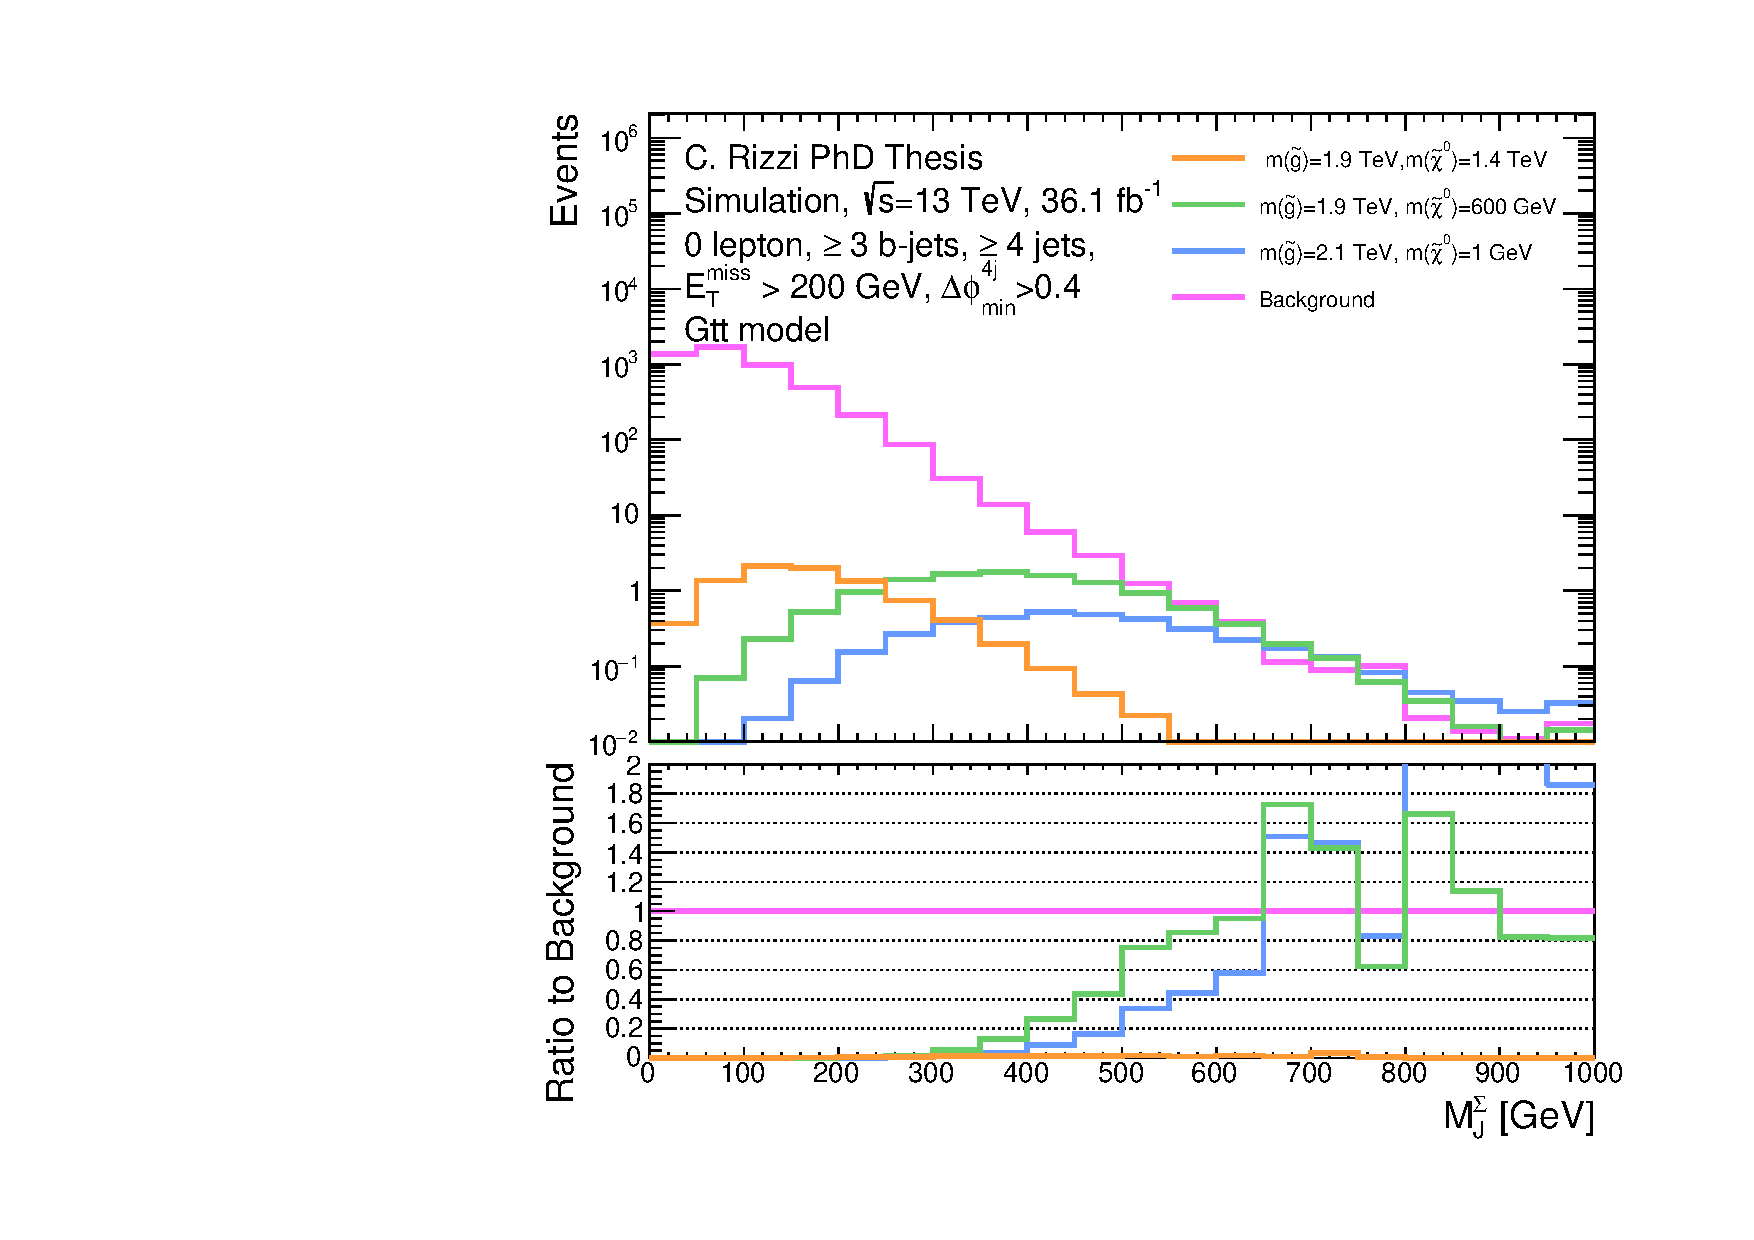
\includegraphics[width=0.325\textwidth]{figures/strong_prod/sig_bkg_strong/0L_3b/Gtt_compare_MJSum_rc_r08pt10.pdf}\label{fig:strong:sig:MJSum_rc_r08pt10B}}
\subfigure[]{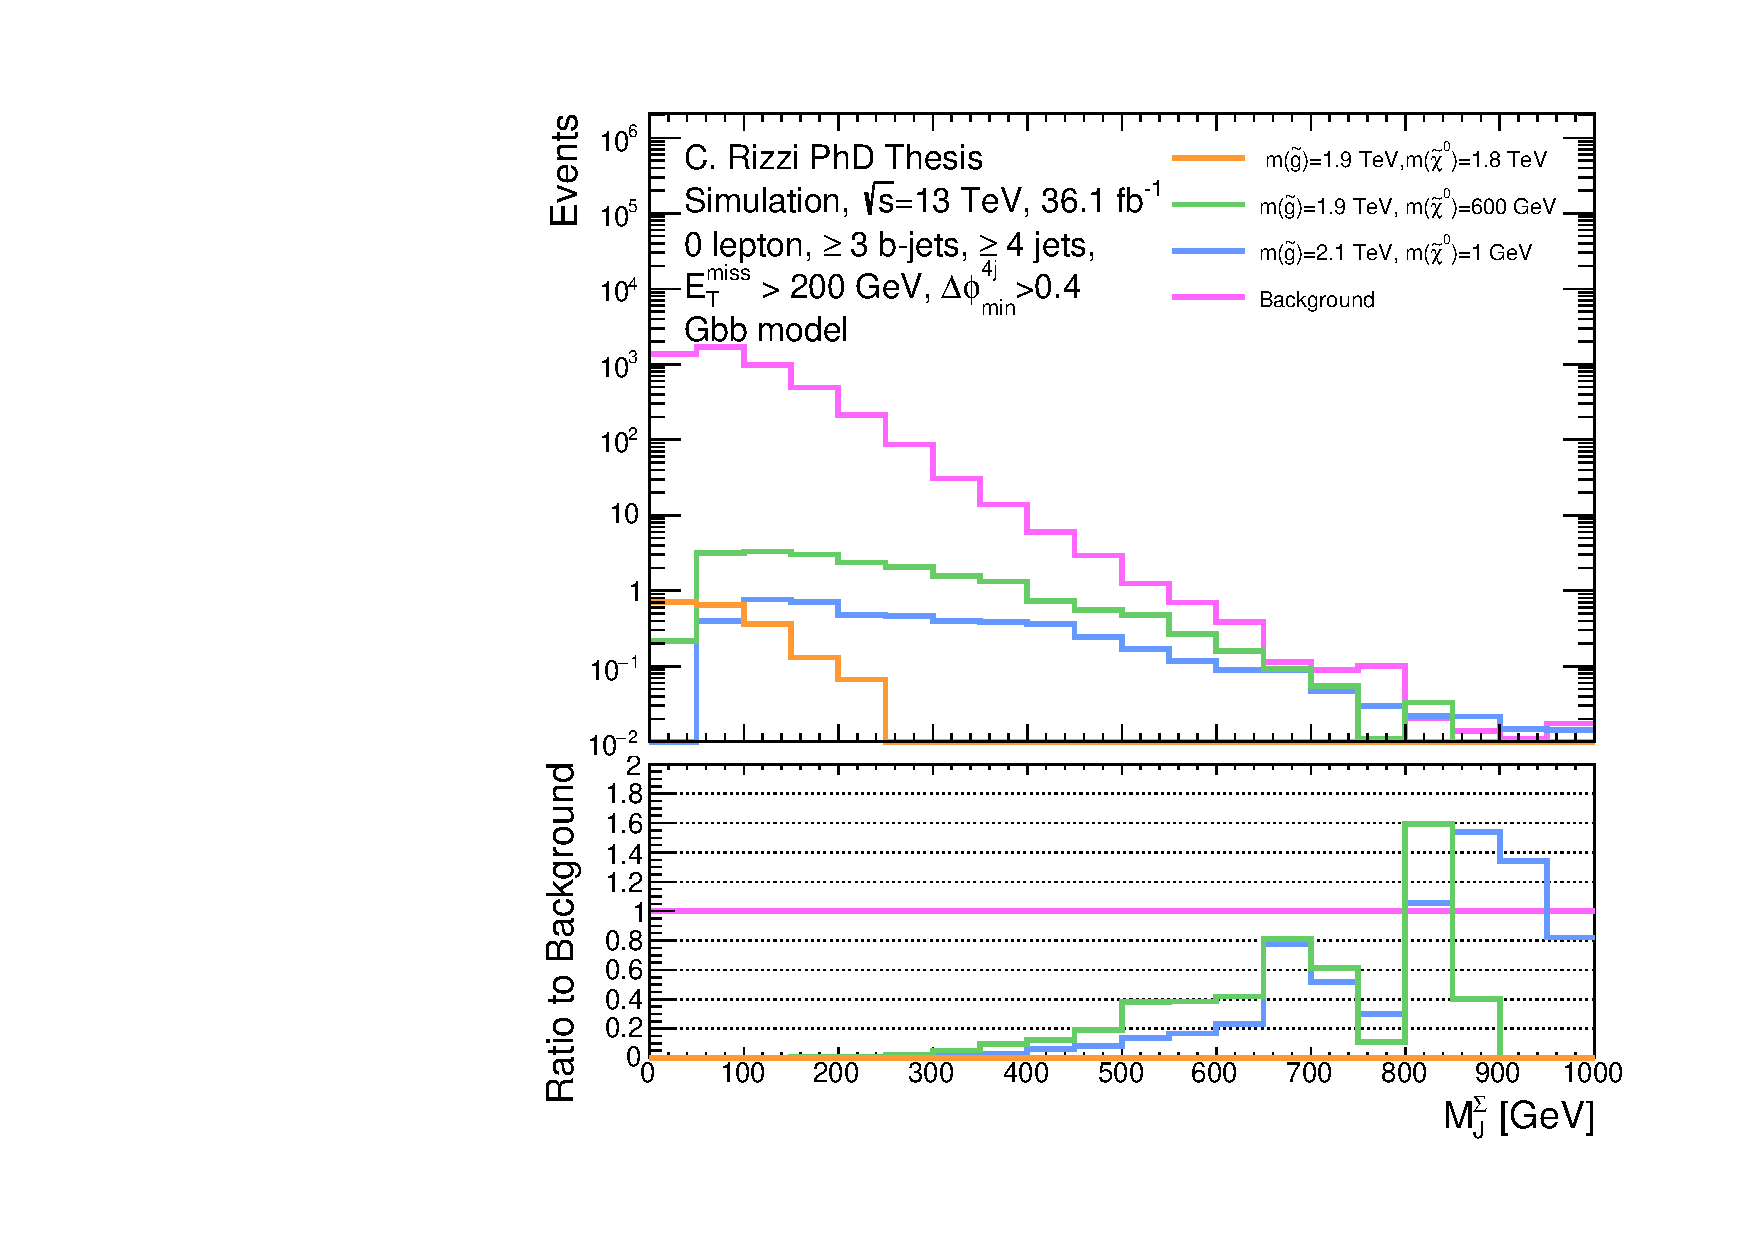
\includegraphics[width=0.325\textwidth]{figures/strong_prod/sig_bkg_strong/0L_3b/Gbb_compare_MJSum_rc_r08pt10.pdf}\label{fig:strong:sig:MJSum_rc_r08pt10C}}
\caption{Distribution of \mjsum in background events and in \subref{fig:strong:sig:MJSum_rc_r08pt10A} Gtt signals in a 1-lepton selection, 
\subref{fig:strong:sig:MJSum_rc_r08pt10B} Gtt signals in a  0-lepton selection and
\subref{fig:strong:sig:MJSum_rc_r08pt10C} Gbb signals in a  0-lepton selection.
}\label{fig:strong:sig:MJSum_rc_r08pt10}
\end{figure*}


\begin{figure*}[htbp]
\centering 
\subfigure[]{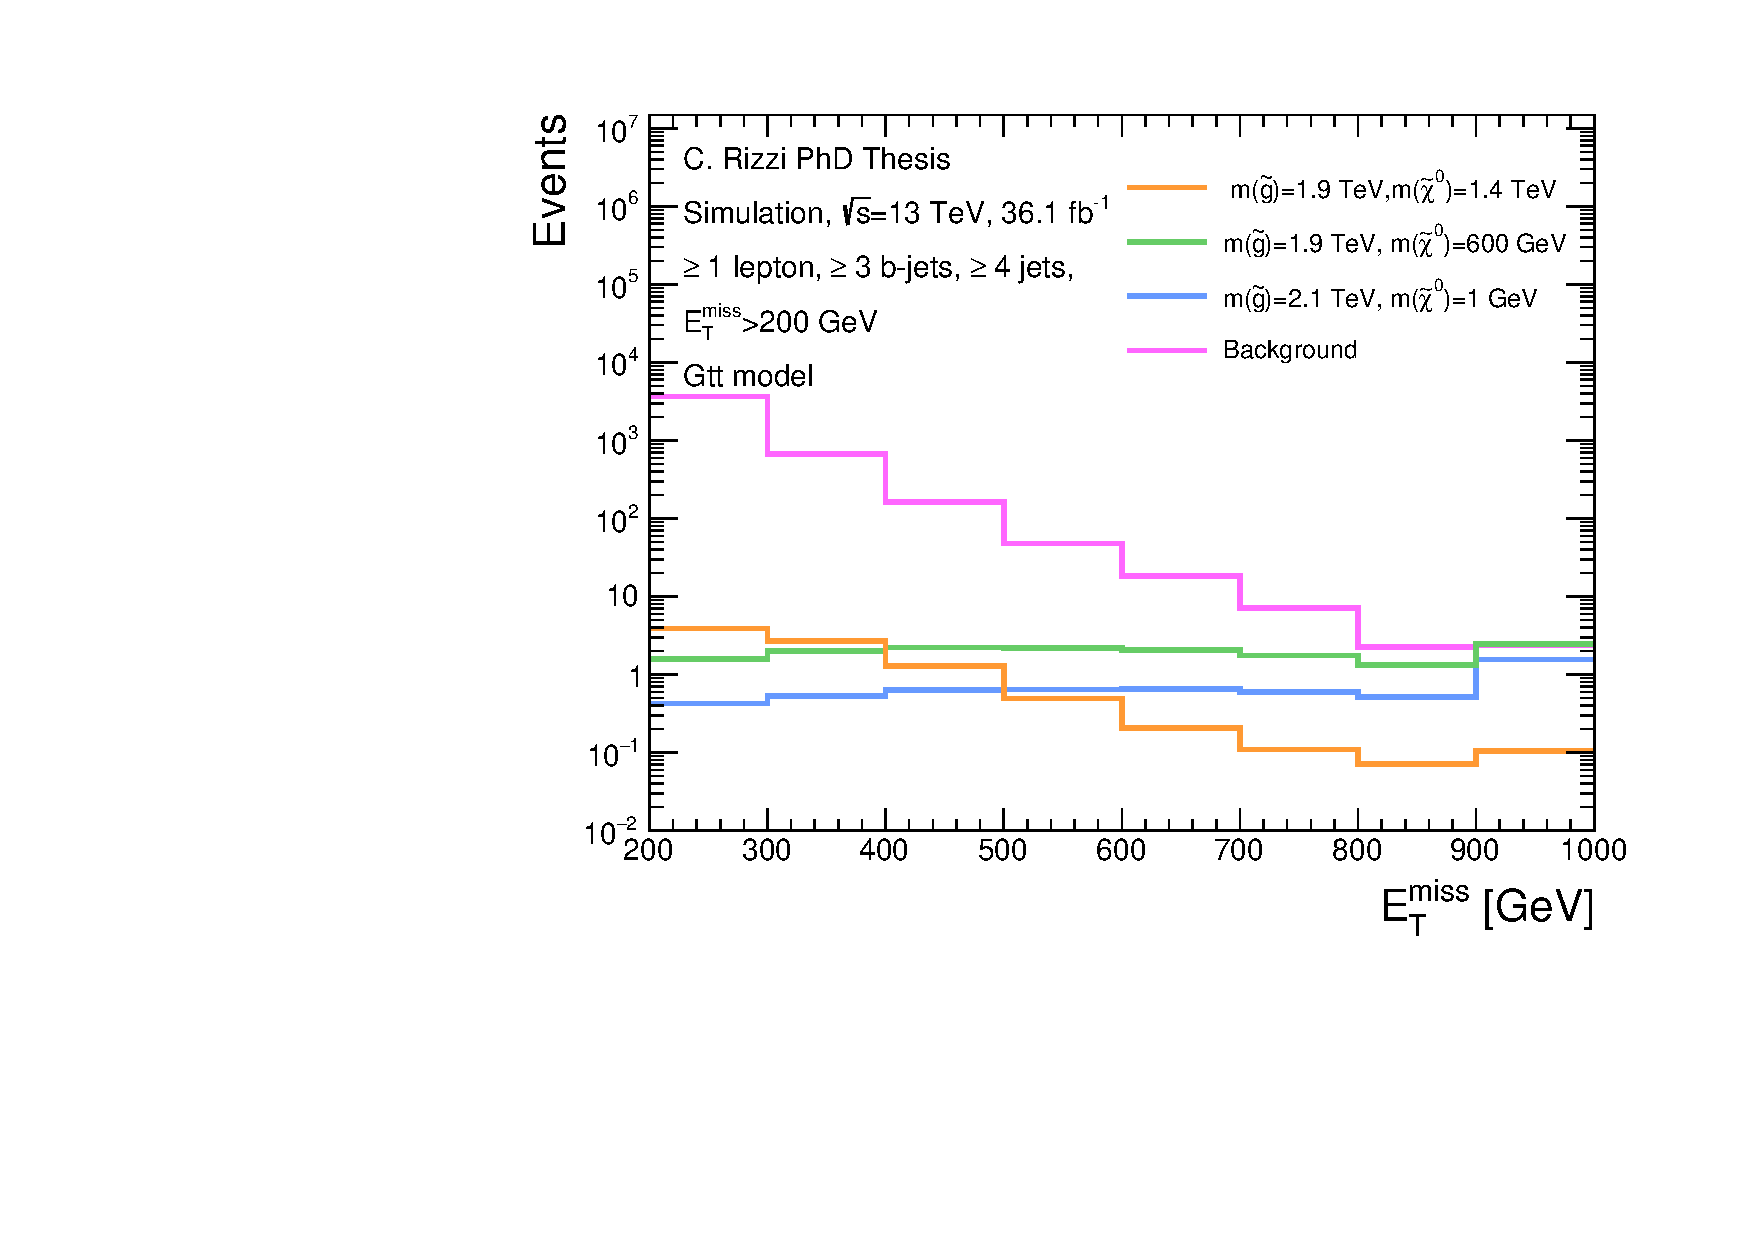
\includegraphics[width=0.325\textwidth]{figures/strong_prod/sig_bkg_strong/1L_3b/Gtt_compare_met.pdf}\label{fig:strong:sig:metA}}
\subfigure[]{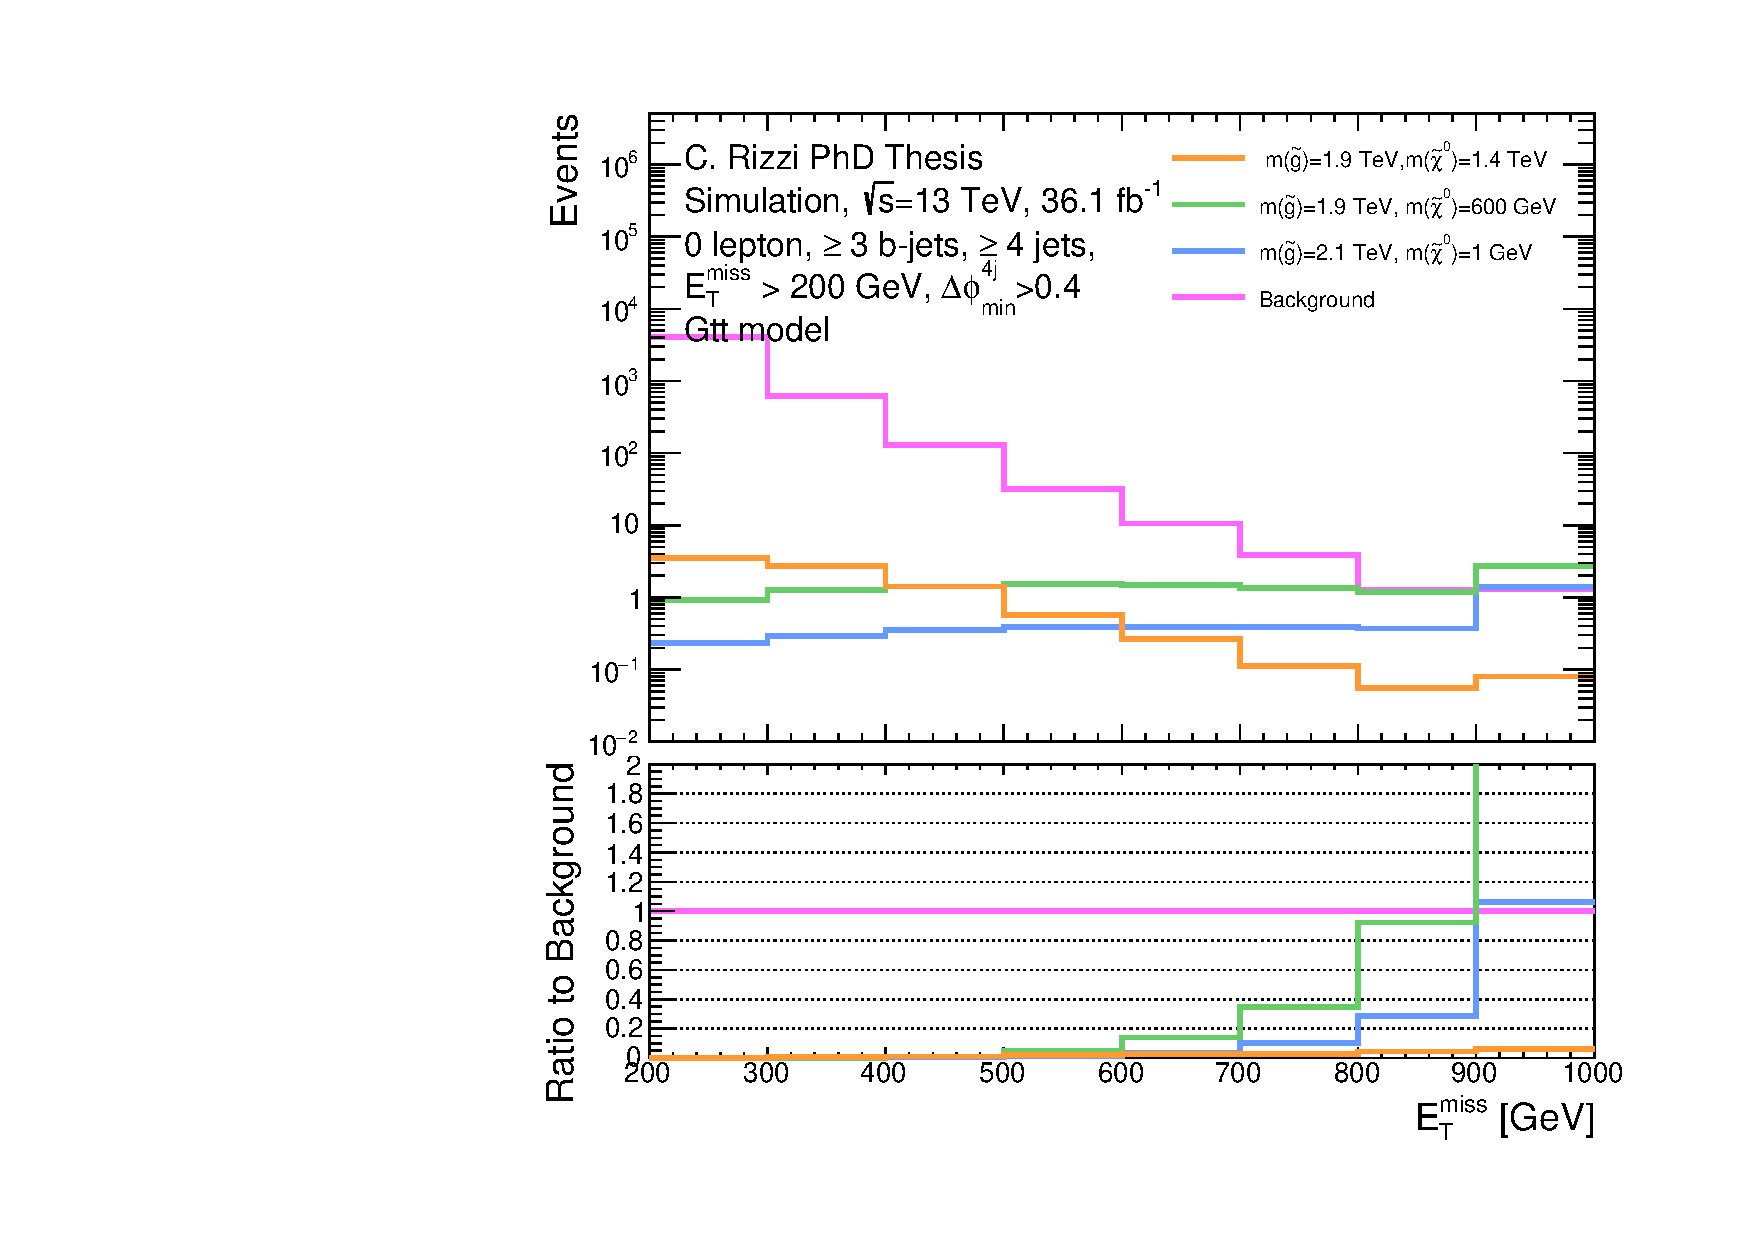
\includegraphics[width=0.325\textwidth]{figures/strong_prod/sig_bkg_strong/0L_3b/Gtt_compare_met.pdf}\label{fig:strong:sig:metB}}
\subfigure[]{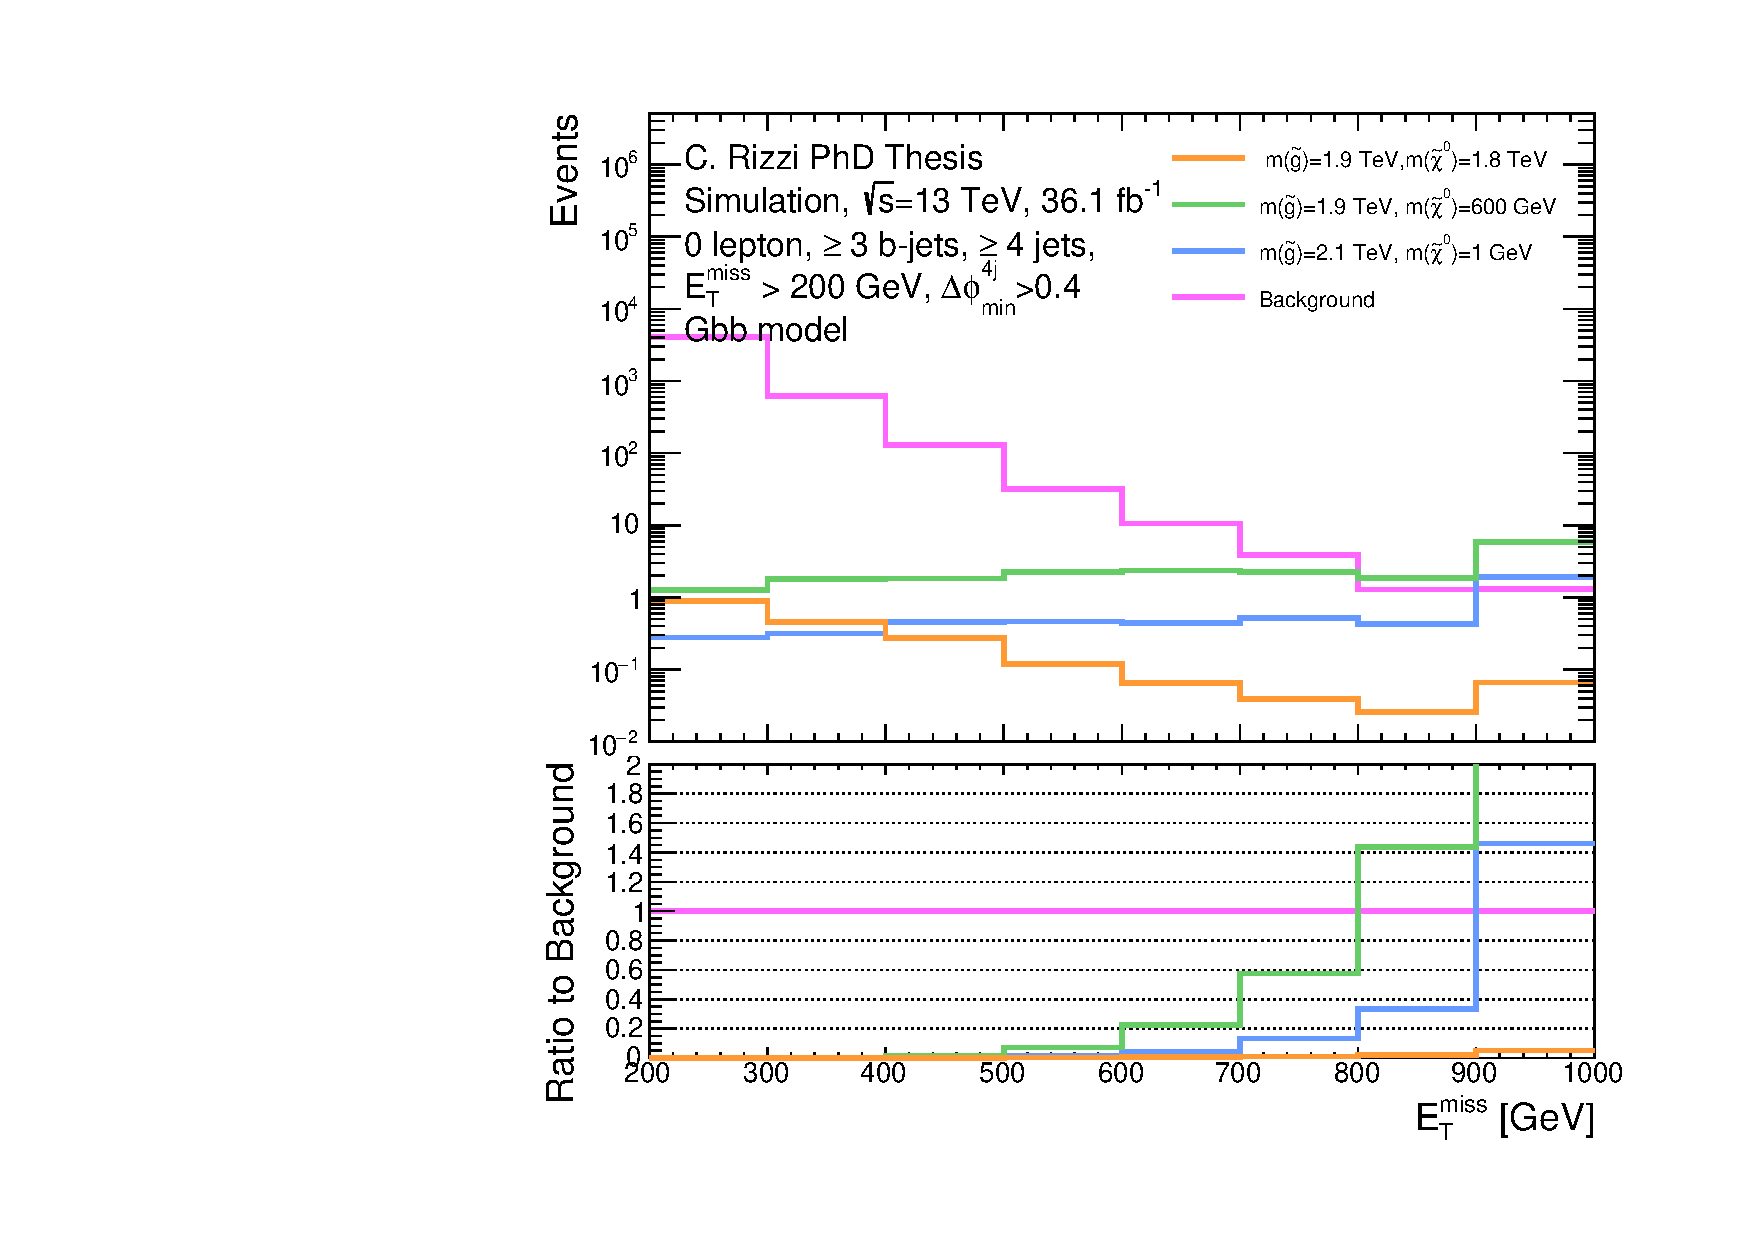
\includegraphics[width=0.325\textwidth]{figures/strong_prod/sig_bkg_strong/0L_3b/Gbb_compare_met.pdf}\label{fig:strong:sig:metC}}
\caption{Distribution of \met in  background events and in \subref{fig:strong:sig:metA} Gtt signals in a 1-lepton selection, 
\subref{fig:strong:sig:metB} Gtt signals in a  0-lepton selection
 and \subref{fig:strong:sig:metC} Gbb signals in a  0-lepton selection.
}\label{fig:strong:sig:met}
\end{figure*}

\FloatBarrier

\section{Cut-and-count analysis regions}
\label{sec:strong:cutandcount}
In this section, we discuss the definition of the cut-and-count analysis regions: 
first of all the optimization process that leads to the \glspl{sr} and then the 
design of corresponding \glspl{cr} for the normalization of the \ttbar background and 
\glspl{vr} to test the validity of the background prediction.

\subsection{Signal regions}

As discussed in Section \ref{sec:analysisstrategy}, the cut-and-count \glspl{sr} are designed to maximize the significance to specific 
signal benchmarks, where the significance is defined as the number of standard deviations in a Gaussian that give the p-value obtained with Equation \ref{eq:binomexpp}.
Since they are not meant to be statistically combined, they do not need to be mutually exclusive and each of them can be optimized independently.
The variables considered in the optimization are chosen by selecting the ones that show the most significant differences in shape between signal and background, and are \njet, \nbjet, \met, \meff, \mjsum, \mtb and, in the case of regions requiring at least one lepton, \mt.
The \glspl{sr} are defined as the set of selections that maximize the expected significance for each benchmark model while fulfilling these requirements:
\begin{itemize}
\item At least 0.5 expected background events.
\item \ttbar as major background component, since it is the one that is normalized in \glspl{cr}.
\item The \gls{mc} statistical uncertainty on the \ttbar component $<30$\%.
\item At least 2 expected events for the benchmark signal considered. 
\end{itemize}
After selecting events with at lest four jets, at least three $b$-jets, which fired the \met trigger and with $\met>200$ GeV, three separate optimizations are performed:

\begin{description}

\item[Gtt-1L] A first set of regions targets the Gtt signals (shown in Figure \ref{fig:diagram_Gtt}) in the final states with at least one reconstructed lepton. Three different \glspl{sr} are defined in this category: boosted (B), targeting signal models with high gluino mass 
and a large mass difference between the gluino and the neutralino, medium (M), targeting signal models with intermediate mass splitting, and compressed (C), aiming at signal models where the mass of the neutralino is close to the mass of the gluino. 

\item[Gtt-0L] A separate optimization is performed for the cases where the Gtt model leads to final states where there are no reconstructed leptons.
Also in this case, three \glspl{sr} are defined and again referred to as B, M and C depending on the signal models they are targeting. 
All the Gtt \glspl{sr} are reported in Table \ref{tab:GttEvsel}, together with their \glspl{cr} and \glspl{sr} whose design is discussed in the next section. 

\item[Gbb] The optimization of the \glspl{sr} targeting the Gbb model (shown in Figure \ref{fig:diagram_Gbb}) is performed separately. 
This signal does not produce any prompt lepton in the final state, but its characteristics differ noticeably from 
the case of Gtt-0L, particularly it has a lower number of jets. 
Four \glspl{sr} are optimized for the Gbb signals: boosted (B), medium (M), compressed (C), and very compressed (VC). 
The last \gls{sr} targets compressed Gbb models, where the ETmiss trigger requirement is satisfied because the gluino system is recoiling against 
and \gls{isr} jet, giving additional boost to the neutralinos. To enhance this topology, this region requires that the leading jet is
not $b$-tagged, and 
the variable \dphilead is included in the optimization. The selections resulting from the optimization of the Gbb \glspl{sr} are 
reported in Table \ref{tab:Gbb0LEvsel}, together with the corresponding \glspl{cr} and \glspl{vr}.

\end{description}

\subsection{Control and validation regions}

All the \glspl{cr} of the cut-and-count regions, including the ones for the Gbb \glspl{sr} and for the Gtt-1L \glspl{sr}
require the presence of at least one signal lepton. 
The orthogonality with the Gtt-1L \glspl{sr} is ensured by applying to all the \glspl{cr} an upper selection on $\mt < 150$ GeV.
To have enough statistics in the \glspl{cr} to properly constrain the \ttbar background, the 
\mtb selection is removed and other selections are relaxed, ensuring at least 10 expected background events in each \gls{cr}.

In the Gtt-1L regions the extrapolation between each pair of \gls{cr} and \gls{sr} is validated in two different \glspl{vr}:
\gls{vr}-\mt is designed to verify the extrapolation to high \mt, and is maintained orthogonal to the \gls{sr} through an inverted \mjsum 
selection. A second region, \gls{vr}-\mtb, tests the extrapolation to high \mtb by selecting events with high \mtb and low \mt; 
this region is orthogonal to the corresponding \gls{cr} thanks to the exclusive jet multiplicity requirement that characterizes
the Gtt-1L \glspl{cr}.

In the case of the Gtt-0L regions, the main extrapolation between each pair of \gls{cr} and \gls{sr} is on the number of leptons. 
This is validated in a specifically-designed 0-lepton \gls{vr}, 
that is kept orthogonal to the corresponding \gls{sr} by an inverted \mjsum selection.

Similarly, also each Gbb region has a 0-lepton \gls{vr}, whose orthogonality with the \gls{sr} is maintained through 
a shift in the \meff selection for Gbb-B and Gbb-M, and in the \met selection in Gbb-C and Gbb-VC (since these last 
two regions target signal models with a compressed mass spectrum, and therefore do not apply any \meff selection in the \gls{sr}).



\begin{table}[htbp]
    \centering
 \renewcommand{\arraystretch}{1.5}
         \begin{tabular}{c c c c c c c c}
        \toprule
\multicolumn{8}{c}{\textbf{ Gtt-1L}}\\
\multicolumn{8}{c}{Criteria common to all regions: $\ge 1$ signal lepton, ${\pt}^\mathrm{jet} >  30~\gev$, $\nbjet \geq 3$} \\\midrule
Targeted kinematics & Type & $\njet$ & $\mt$ & $\mtb$& $\met$ & $\meffi$ & $\mjsum$ \\ \midrule
\multirow{4}{*}{\begin{minipage}{3cm}\centering Region B\\
              (Boosted, Large \msplit) \end{minipage}} 
 & SR & $\ge 5$ & $> 150$ & $> 120 $  & $> 500 $ & $> 2200 $ & $> 200$  \\
 & CR & $= 5$ & $< 150$ & $-$  & $> 300 $ & $> 1700 $ & $> 150$  \\
 & VR-$\mt$ & $\ge 5$ & $> 150$ & $-$  & $> 300 $ & $> 1600 $ & $< 200$  \\
& VR-$\mtb$ & $> 5$ & $< 150$ & $> 120 $  & $> 400 $ & $> 1400 $ & $> 200$  \\\midrule
\multirow{4}{*}{\begin{minipage}{3cm}\centering Region M\\
              (Moderate \msplit) \end{minipage}} 
 & SR & $\ge 6$ & $> 150$ & $> 160 $  & $> 450 $ & $> 1800 $ & $> 200$  \\
 & CR & $= 6$ & $< 150$ & $-$  & $> 400 $ & $> 1500 $ & $> 100$  \\
 & VR-$\mt$ & $\ge 6$ & $> 200$ & $-$  & $> 250 $ & $> 1200 $ & $< 100$  \\
& VR-$\mtb$ & $> 6$ & $< 150$ & $> 140 $  & $> 350 $ & $> 1200 $ & $> 150$  \\\midrule
\multirow{4}{*}{\begin{minipage}{3cm}\centering Region C\\
              (Compressed, small \msplit) \end{minipage}} 
 & SR & $\ge 7$ & $> 150$ & $> 160 $  & $> 350 $ & $> 1000 $ & $-$  \\
 & CR & $= 7$ & $< 150$ & $-$  & $> 350 $ & $> 1000 $ & $-$  \\
 & VR-$\mt$ & $\ge 7$ & $> 150$ & $< 160 $  & $> 300 $ & $> 1000 $ & $-$  \\
& VR-$\mtb$ & $> 7$ & $< 150$ & $> 160 $  & $> 300 $ & $> 1000 $ & $-$  \\
      \end{tabular}
         \begin{tabular}{c c c c c c c c c c c}
        \toprule
\multicolumn{11}{c}{\textbf{ Gtt-0L}}\\
\multicolumn{11}{c}{Criteria common to all regions: ${\pt}^\mathrm{jet} > 30$~GeV} \\\midrule
Targeted kinematics & Type & $N_\mathrm{lepton}$ & $\nbjet$& $\njet$&  $\dphimin$ & $\mt$ & $\mtb$ & $\met$ & $\meffi$ & $\mjsum$ \\ \midrule
\multirow{3}{*}{\begin{minipage}{3cm}\centering Region B\\
              (Boosted, Large \msplit) \end{minipage}} 
& SR & $= 0$  & $\ge 3$ & $\ge 7$ & $>0.4$ & $-$ & $> 60 $ & $> 350 $ & $> 2600$ & $> 300$\\ 
& CR & $= 1$  & $\ge 3$ & $\ge 6$ & $-$ & $<150$ & $-$ & $> 275 $ & $> 1800$ & $> 300$\\ 
& VR & $= 0$  & $\ge 3$ & $\ge 6$ & $>0.4$ & $-$ & $-$ & $> 250 $ & $> 2000$ & $< 300$\\ \midrule
\multirow{3}{*}{\begin{minipage}{3cm}\centering Region M\\
              (Moderate \msplit) \end{minipage}} 
& SR & $= 0$  & $\ge 3$ & $\ge 7$ & $>0.4$ & $-$ & $> 120 $ & $> 500 $ & $> 1800$ & $> 200$\\ 
& CR & $= 1$  & $\ge 3$ & $\ge 6$ & $-$ & $<150$ & $-$ & $> 400 $ & $> 1700$ & $> 200$\\ 
& VR & $= 0$  & $\ge 3$ & $\ge 6$ & $>0.4$ & $-$ & $-$ & $> 450 $ & $> 1400$ & $< 200$\\ \midrule
\multirow{3}{*}{\begin{minipage}{3cm}\centering Region C\\
              (Compressed, moderate \msplit) \end{minipage}} 
& SR & $= 0$  & $\ge 4$ & $\ge 8$ & $>0.4$ & $-$ & $> 120 $ & $> 250 $ & $> 1000$ & $> 100$\\ 
& CR & $= 1$  & $\ge 4$ & $\ge 7$ & $-$ & $<150$ & $-$ & $> 250 $ & $> 1000$ & $> 100$\\ 
& VR & $= 0$  & $\ge 4$ & $\ge 7$ & $>0.4$ & $-$ & $-$ & $> 250 $ & $> 1000$ & $< 100$\\ 

\bottomrule
\end{tabular}
\caption{Definitions of the Gtt SRs, CRs and VRs of the cut-and-count analysis.  All kinematic variables are
   expressed in \gev\ except $\dphimin$, which is in radians. The jet \pt\ requirement is also applied to 
   $b$-tagged jets. Table from Ref. \cite{Aaboud:2017hrg}.}
      \label{tab:GttEvsel}
 \end{table}

%\clearpage


\begin{landscape}
\begin{table}[htbp]
%\begin{sidewaystable}[t]
    \centering
 \renewcommand{\arraystretch}{1.3}
         \begin{tabular}{c c c c c c c c c c}
        \toprule
\multicolumn{10}{c}{\textbf{ Gbb}}\\
\multicolumn{10}{c}{Criteria common to all regions: $\njet \geq 4$,
           ${\pt}^\mathrm{jet} > 30$~GeV } \\\midrule 
Targeted kinematics  & Type & $N_\mathrm{lepton}$ & $\nbjet$ &  $\dphimin$ & $\mt$ & $\mtb$ & $\met$ & $\meff$ & Others  \\\midrule
\multirow{3}{*}{\begin{minipage}{3cm}\centering Region B\\
              (Boosted, Large \msplit) \end{minipage}} 
& SR & $= 0$  & $\ge 3$ & $>0.4$ & $-$ & $- $ & $> 400 $ & $> 2800$ & $-$ \\ 
& CR & $= 1$  & $\ge 3$ & $-$ & $< 150$ & $- $ & $> 400 $ & $> 2500$ & $-$ \\ 
& VR & $= 0$  & $\ge 3$ & $>0.4$ & $-$ & $- $ & $> 350 $ & $1900$--$2800$ & $-$ \\\midrule
\multirow{3}{*}{\begin{minipage}{3cm}\centering Region M\\
              (Moderate \msplit) \end{minipage}} 
& SR & $= 0$  & $\ge 4$ & $>0.4$ & $-$ & $>90$ & $> 450 $ & $> 1600$ & $-$ \\ 
& CR & $= 1$  & $\ge 4$ & $-$ & $< 150$ & $- $ & $> 300 $ & $> 1600$ & $-$ \\ 
& VR & $= 0$  & $\ge 4$ & $>0.4$ & $-$ & $>100$ & $250$--$450$ & $1600$--$1900$ & $-$ \\\midrule
\multirow{3}{*}{\begin{minipage}{3cm}\centering Region C\\
              (Compressed, small \msplit) \end{minipage}} 
& SR & $= 0$  & $\ge 4$ & $>0.4$ & $-$ & $>155$ & $> 450 $ & $-$ & $-$ \\ 
& CR & $= 1$  & $\ge 4$ & $-$ & $< 150$ & $- $ & $> 375 $ & $-$ & $-$ \\ 
& VR & $= 0$  & $\ge 4$ & $>0.4$ & $-$ & $>125$ & $350$--$450$ & $-$ & $-$ \\\midrule
\multirow{3}{*}{\begin{minipage}{3cm}\centering Region VC\\
              (Very Compressed, very small \msplit) \end{minipage}} 
& SR & $= 0$  & $\ge 3$ & $>0.4$ & $-$ & $>100$ & $> 600 $ & $-$ &
                                                                   \multirow{3}{*}{\begin{minipage}{3cm}\centering $\pt^{\leadjet}>400$, $\leadjet \neq b$, $\dphilead>2.5$\end{minipage}} \\ 
& CR & $= 1$  & $\ge 3$ & $-$ & $< 150$ & $- $ & $> 600 $ & $-$ \\ 
& VR & $= 0$  & $\ge 3$ & $>0.4$ & $-$ & $>100$ & $225$--$600$ & $-$ \\
      \bottomrule
    \end{tabular}
      \caption{Definitions of the Gbb SRs, CRs and VRs of the cut-and-count analysis.  
  All kinematic variables are expressed in \gev\ except $\dphimin$, which is in radians.
   The jet \pt\ requirement is applied to the 
   four leading jets, a subset of which are $b$-tagged jets. 
   The $\leadjet \neq b$  requirement specifies that the leading jet is not $b$-tagged.  Table from Ref. \cite{Aaboud:2017hrg}.
   }
       \label{tab:Gbb0LEvsel}
%\end{sidewaystable}
 \end{table}
\end{landscape}



%\clearpage

\subsection{Background composition}

The pre-fit background composition in the the cut-and-count analysis regions is shown in Figures \ref{fig:bkgcomp_Gtt1L}-\ref{fig:bkgcomp_Gbb}.
As can be appreciated, \ttbar is the dominant background in all the \glspl{sr}; the \glspl{cr} and the \glspl{vr} have a high \ttbar 
background purity by construction, since they are designed to respectively normalize this background and validate the extrapolation of this normalization 
in a kinematic regime close to the \glspl{sr}.
% chiara: change, sentence from paper
The subdominant background contributions are single-top, \ttbar+W/Z and, in the 0-lepton channel, Z($\to \nu \nu$)+jets.

%The subdominant background contributions in the 0-lepton regions are Z($\to \nu \nu$)+jets and W($\to \nu$ lepton)+jets events, 
%where for W+jets events the lepton is electron or muon that is not reconstructed or a hadronically decaying $\tau$-lepton. 
%In the 1-lepton \glspl{sr}, the subdominant backgrounds are single-top, \ttbar+W and \ttbar+Z.

\begin{figure}[htbp]
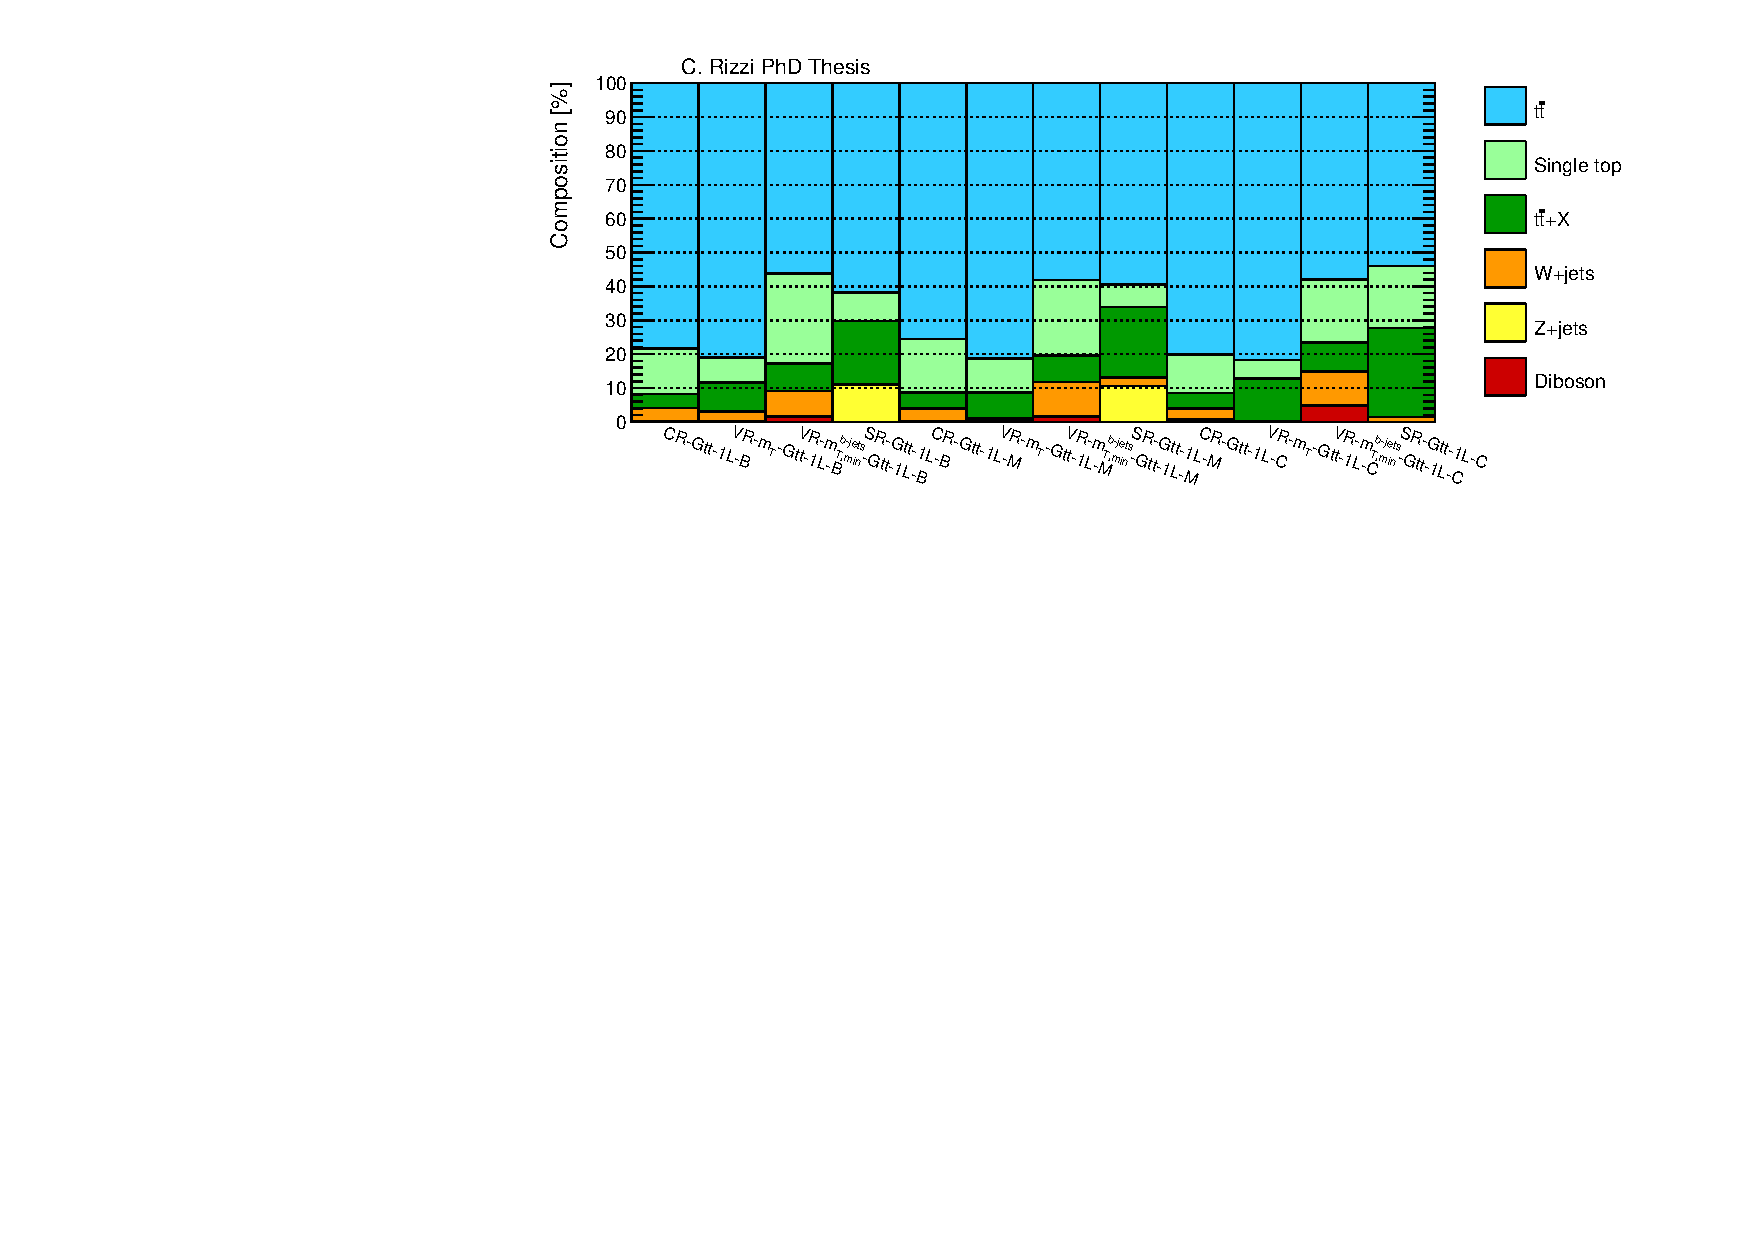
\includegraphics[width=\textwidth]{figures/strong_prod/comp_plots/Gtt_1L_bkg.pdf}
\caption{Background composition in the Gtt-1L regions.}
	\label{fig:bkgcomp_Gtt1L}
\end{figure}

\begin{figure}[htbp]
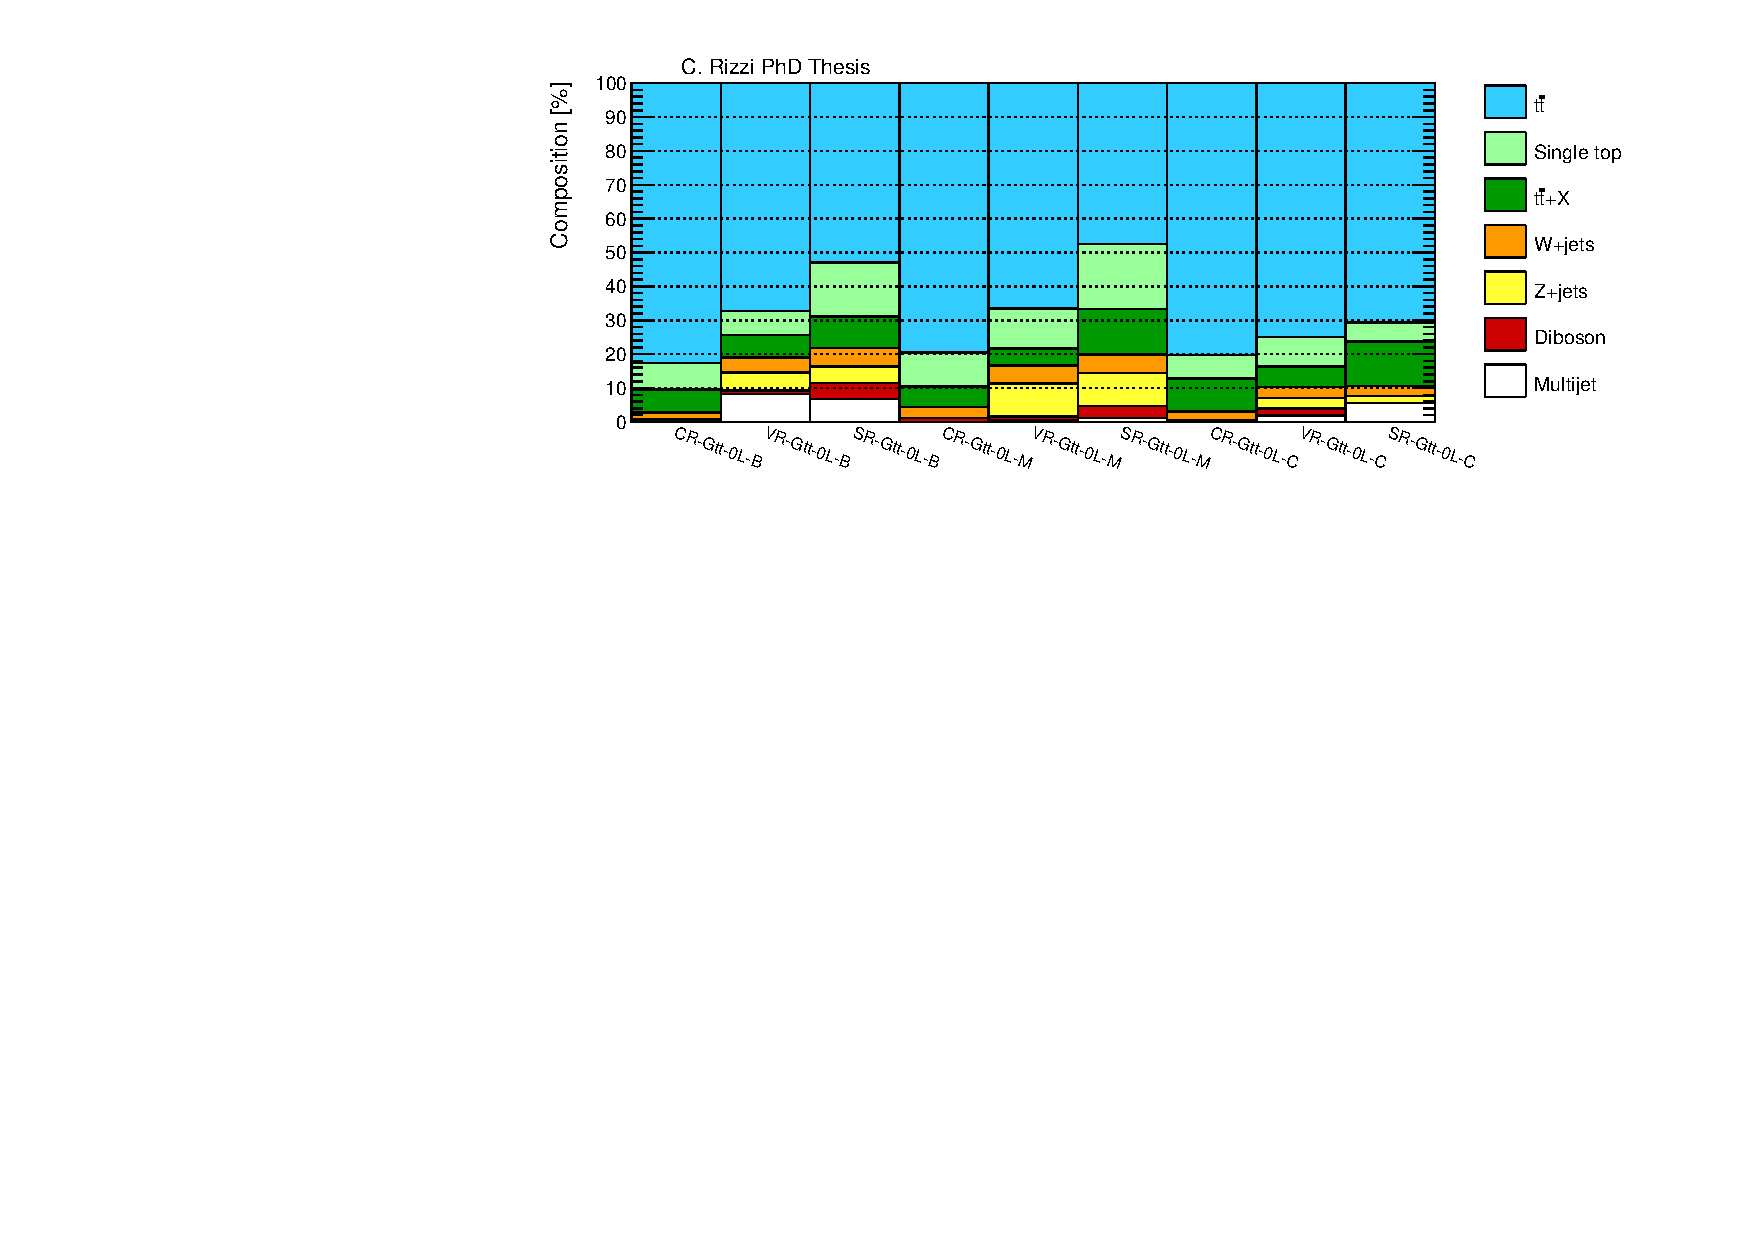
\includegraphics[width=\textwidth]{figures/strong_prod/comp_plots/Gtt_0L_bkg.pdf}
\caption{Background composition in the Gtt-0L regions.}
	\label{fig:bkgcomp_Gtt0L}
\end{figure}

\begin{figure}[htbp]
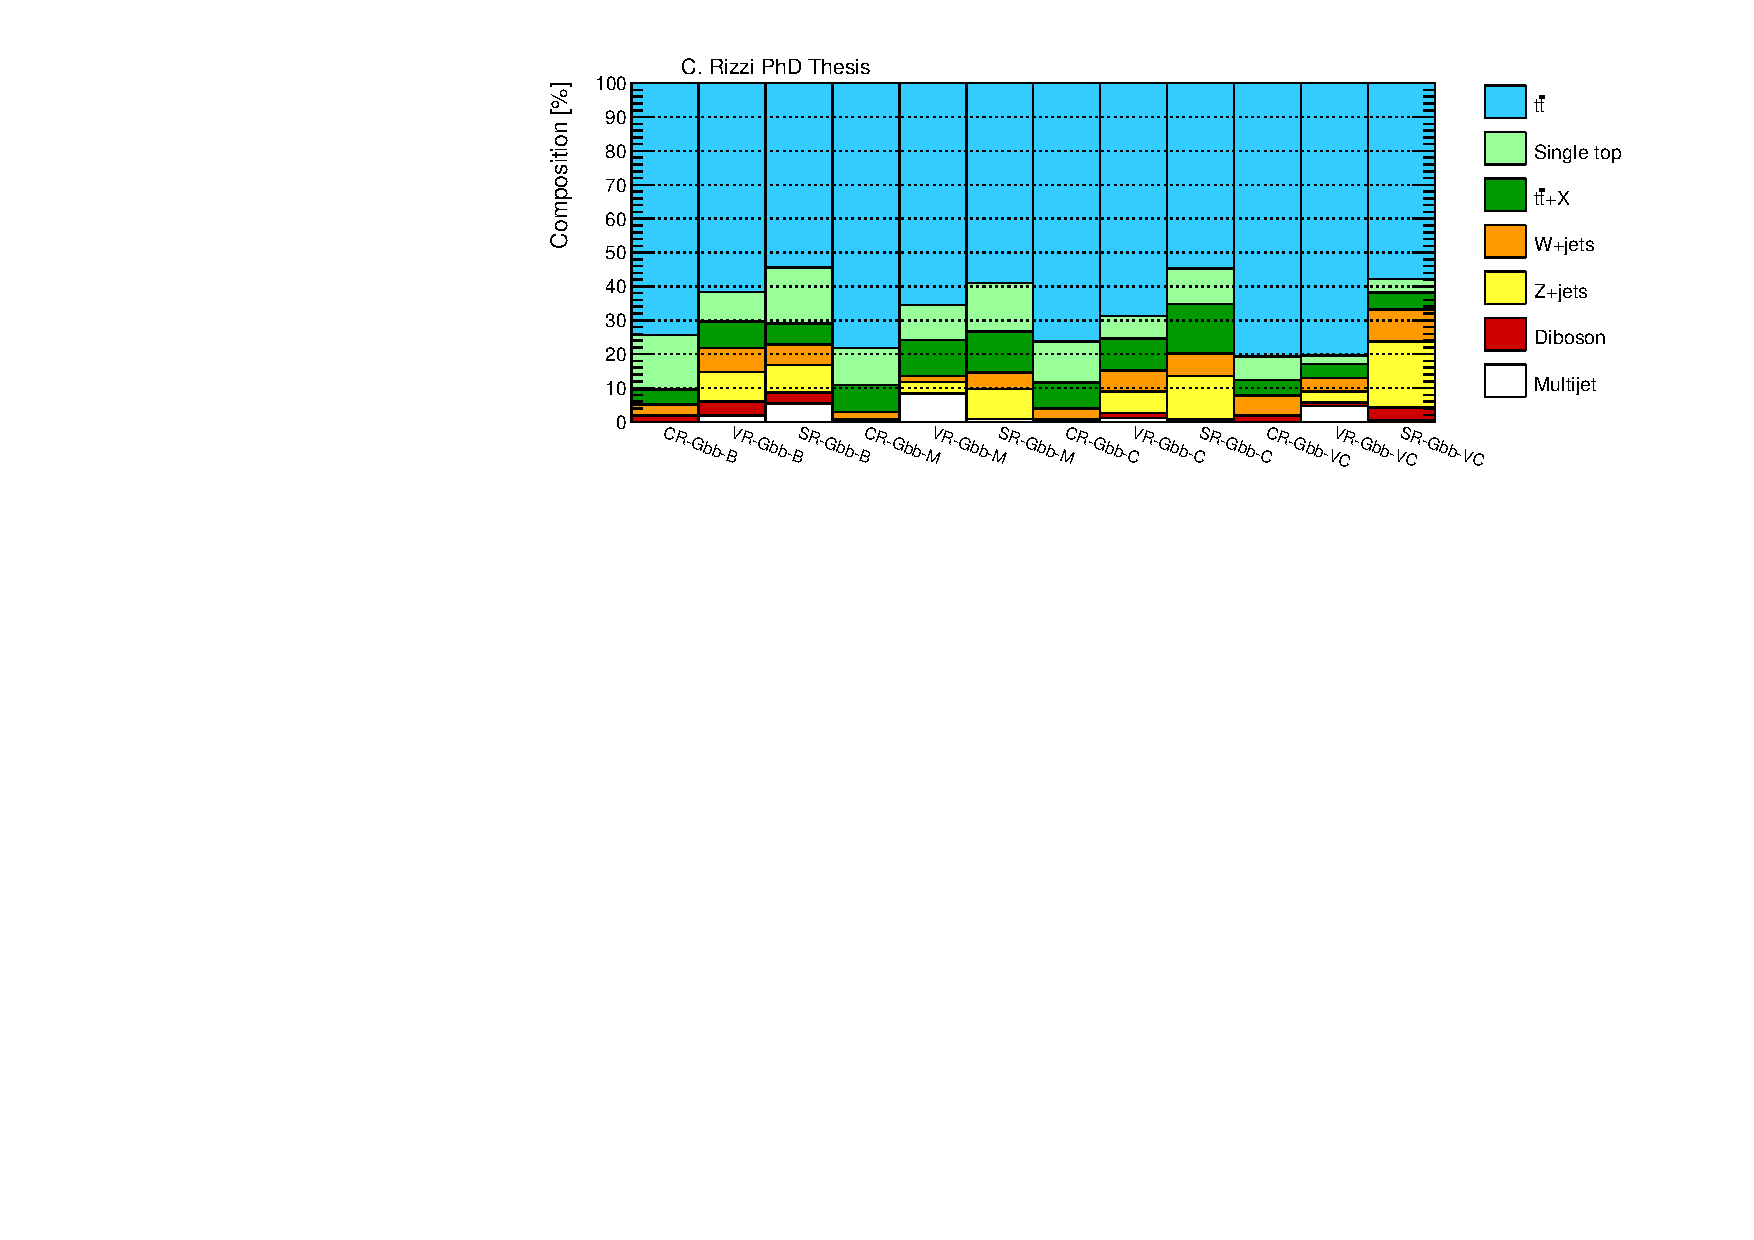
\includegraphics[width=\textwidth]{figures/strong_prod/comp_plots/Gbb_bkg.pdf}
\caption{Background composition in the Gbb regions.}
	\label{fig:bkgcomp_Gbb}
\end{figure}

%%%

Figures \ref{fig:ttcomp_Gtt1L} to \ref{fig:ttcomp_Gbb} show the decay type of the \ttbar background for  Gtt-1L, Gtt-0L and Gbb regions respectively, classified as described in Section \ref{sec:susy_general:ttbar}.
Figure \ref{fig:ttcomp_Gtt1L} shows that the \glspl{cr} are dominated by single-lepton \ttbar background, as well as the \glspl{vr} designed to check the \mtb extrapolation;
this is because both these types of regions have an upper selection on \mt.
Instead the \glspl{sr} and the \glspl{vr} that check the \mt extrapolation require high \mt values;
this selection suppresses single-lepton \ttbar background and therefore the \glspl{sr} and \glspl{vr}-\mt
are dominated by dilepton \ttbar.
In the case of Figures \ref{fig:ttcomp_Gtt0L} and \ref{fig:ttcomp_Gbb} we see all regions are dominated by single-lepton \ttbar background.
In these cases, the \glspl{cr} are 1-lepton regions with an upper cut on \mt and the \glspl{sr} and \glspl{vr} are 0-lepton regions,
so in all of them the main background component is  single-lepton \ttbar. In the case of SRs and VRs though, this single-lepton component
is dominated by $\tau$+jets, since this category includes both hadronic and leptonic decays of the $\tau$-lepton.


\begin{figure}[htbp]
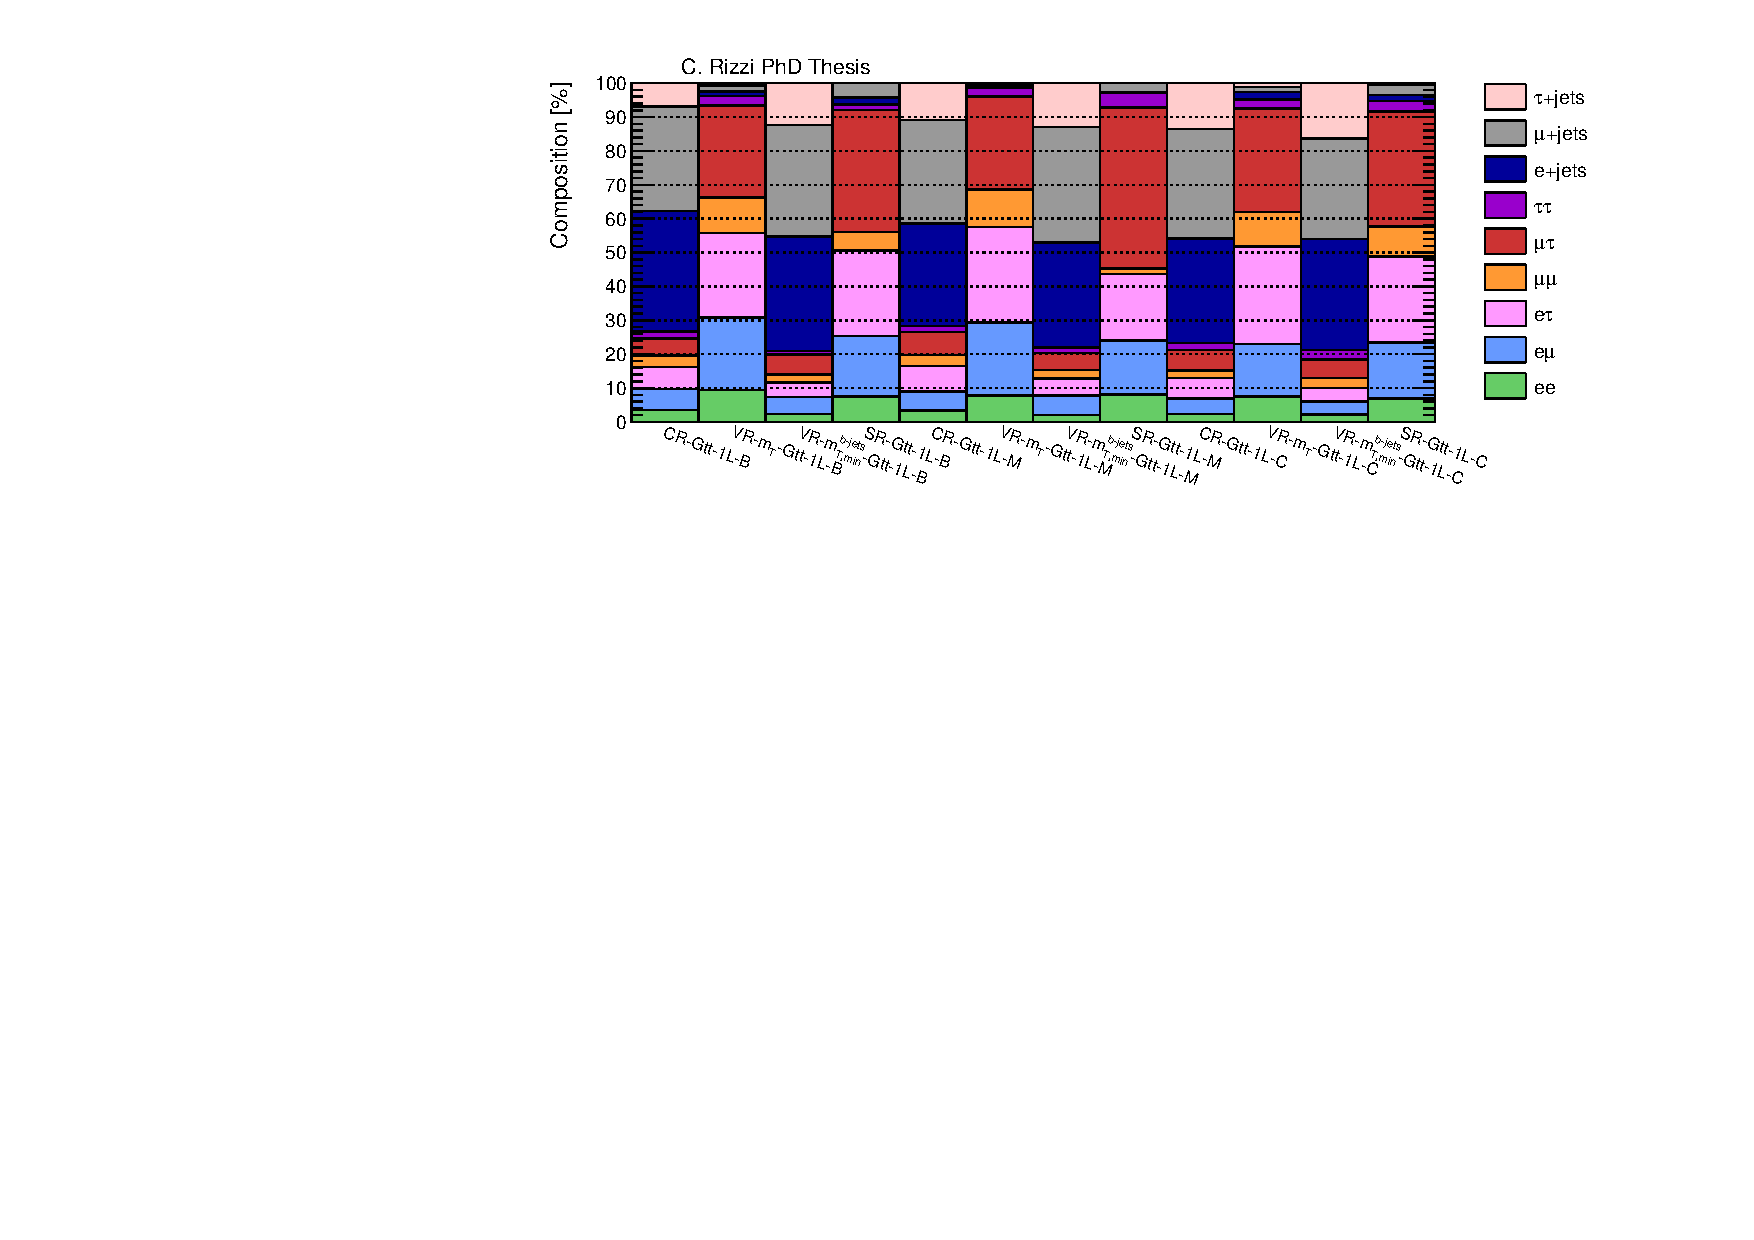
\includegraphics[width=\textwidth]{figures/strong_prod/comp_plots/Gtt_1L_tt.pdf}
\caption{Decay mode of the \ttbar background in the Gtt-1L regions.}
	\label{fig:ttcomp_Gtt1L}
\end{figure}

\begin{figure}[htbp]
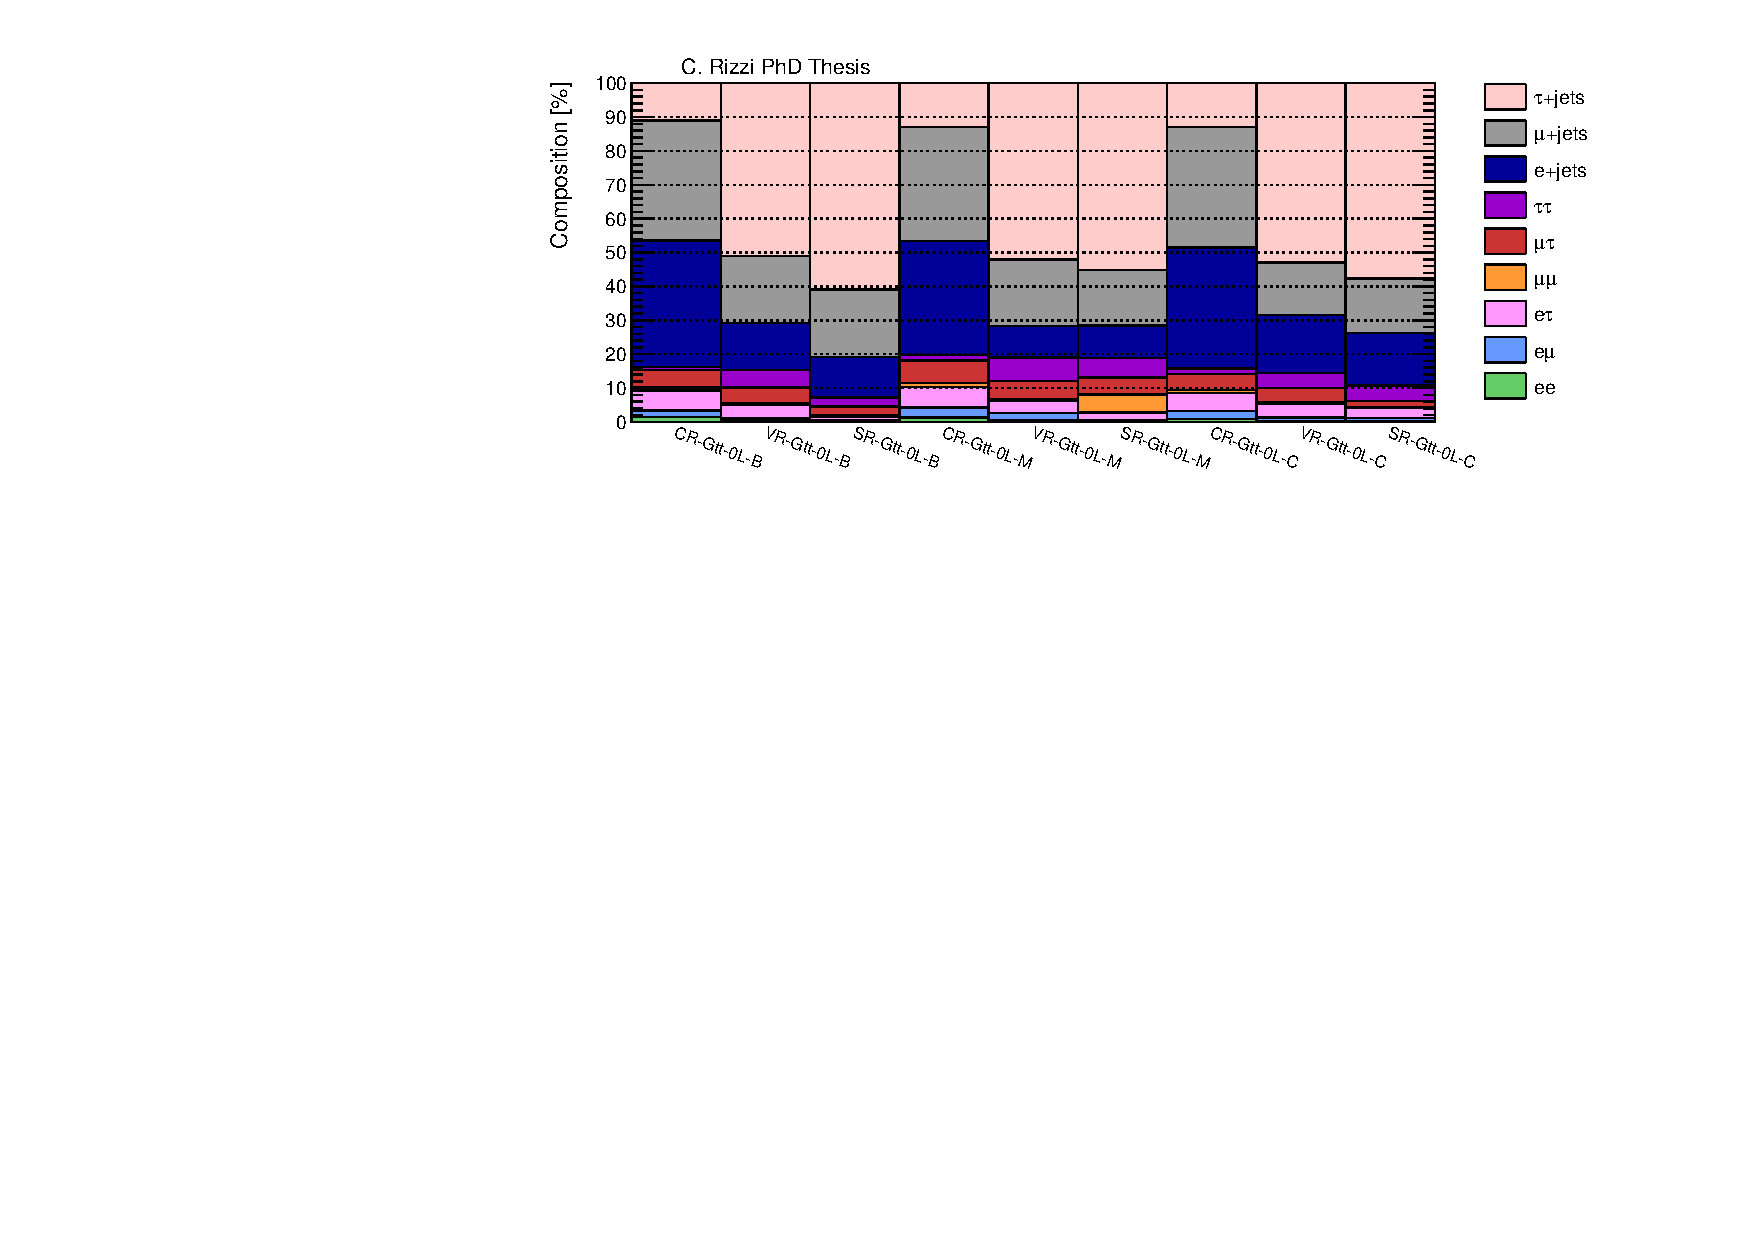
\includegraphics[width=\textwidth]{figures/strong_prod/comp_plots/Gtt_0L_tt.pdf}
\caption{Decay mode of the \ttbar background in the Gtt-0L regions.}
	\label{fig:ttcomp_Gtt0L}
\end{figure}

\begin{figure}[htbp]
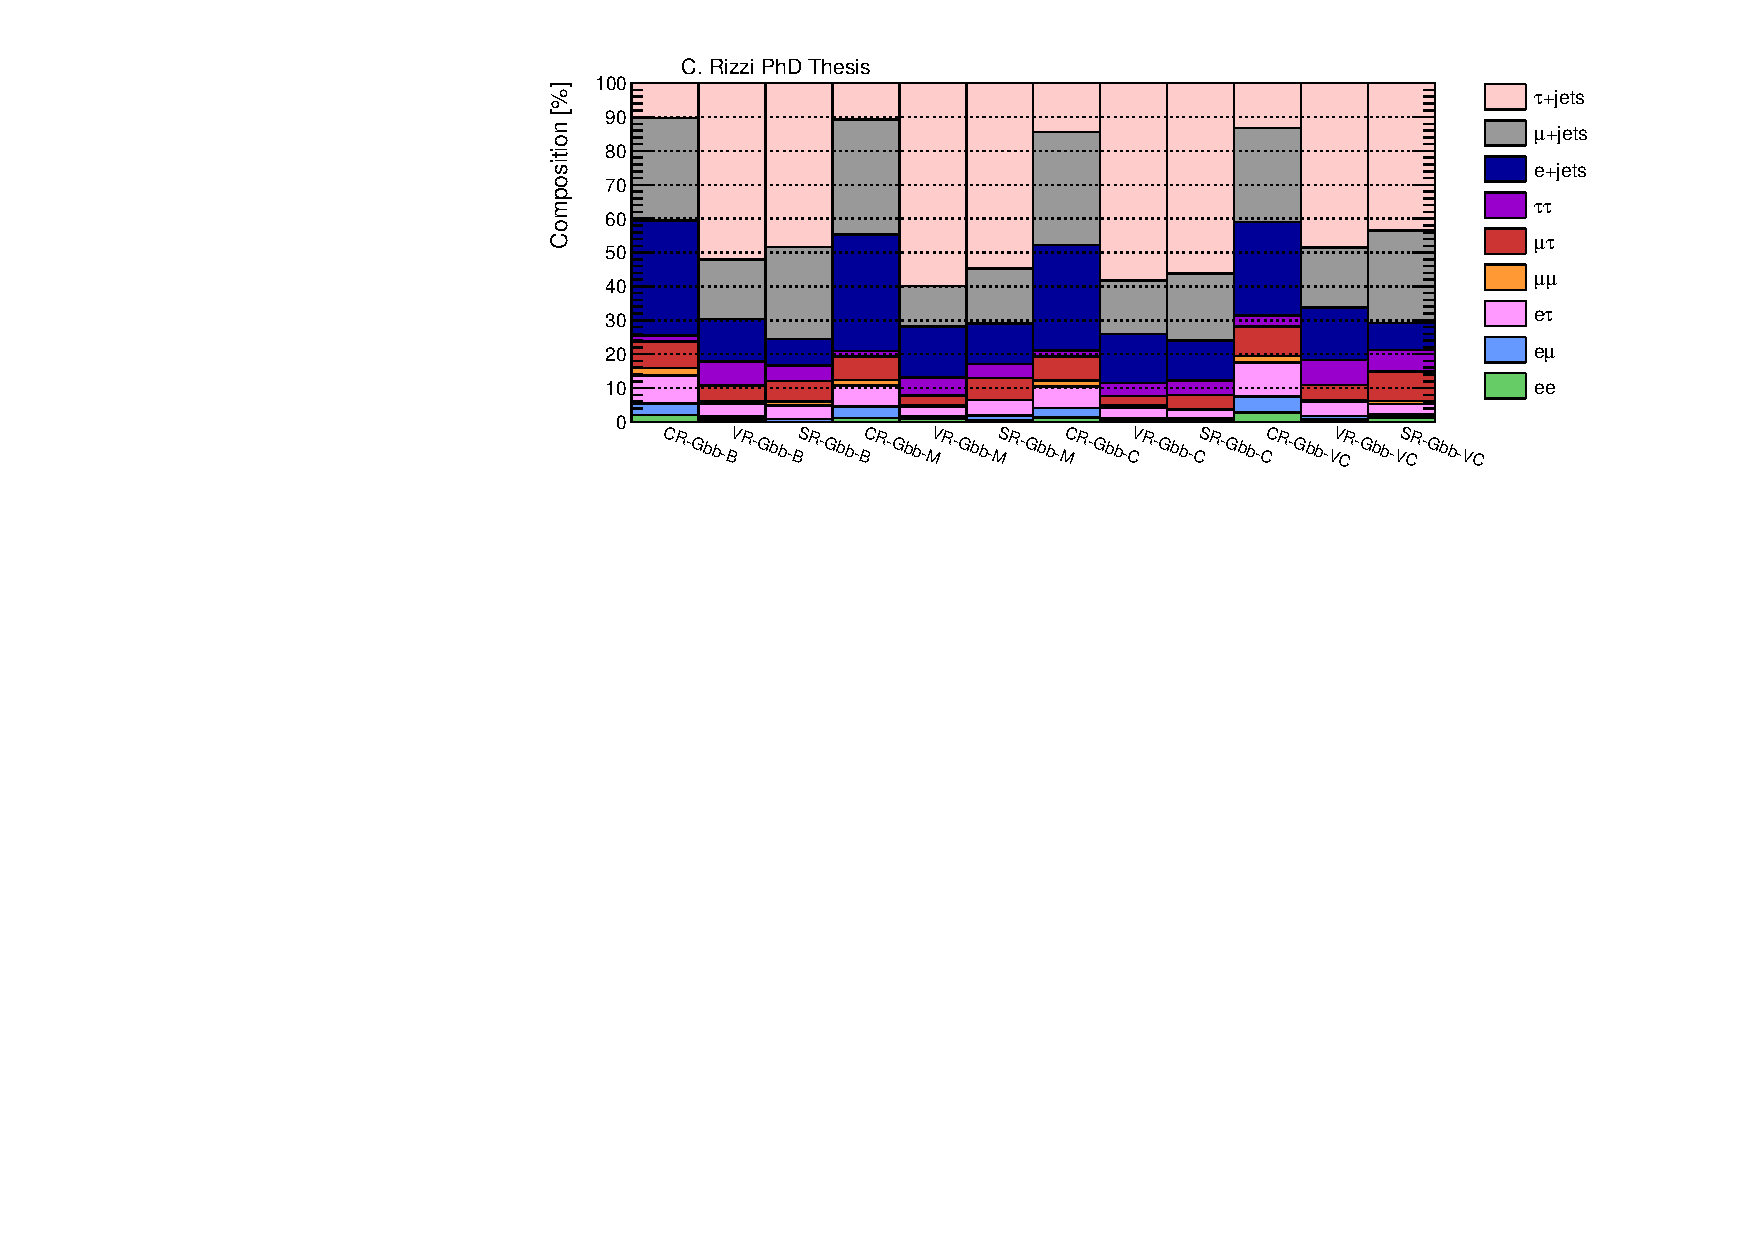
\includegraphics[width=\textwidth]{figures/strong_prod/comp_plots/Gbb_tt.pdf}
\caption{Decay mode of the \ttbar background in the Gbb regions.}
	\label{fig:ttcomp_Gbb}
\end{figure}

%%%%

The classification of the \ttbar background based on the flavour of the jets associated to the 
\ttbar production, as described in Section \ref{sec:susy_general:ttbar}, is shown in Figures 
\ref{fig:HFcomp_Gtt1L}-\ref{fig:HFcomp_Gbb}.
Thanks to adopting the same selection on the number of $b$-jets in \gls{cr}, \gls{sr} and \glspl{vr} 
of the same region type, composition is similar in corresponding regions, even if the fraction of 
\tthf is sometimes higher in the \glspl{sr}, especially in the case of Gtt-1L regions. 


\begin{figure}[htbp]
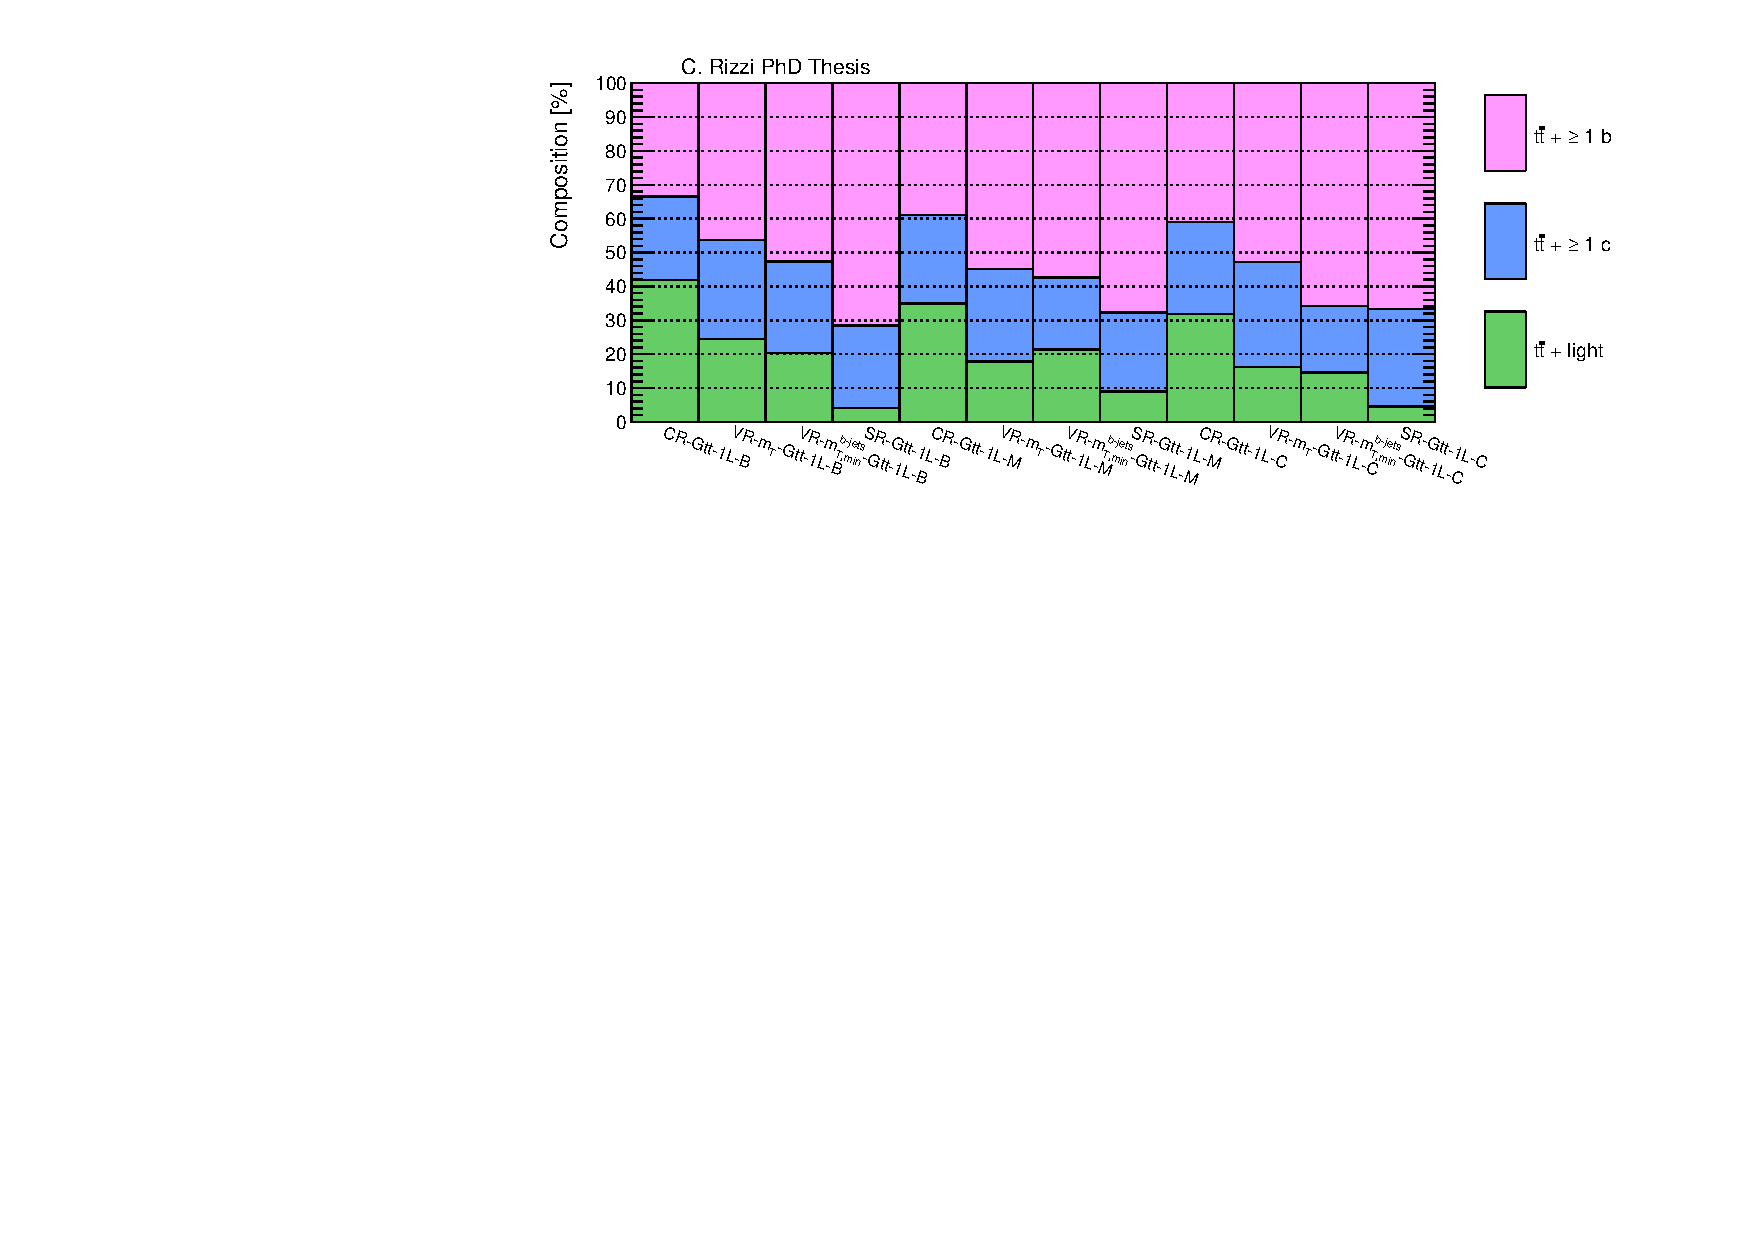
\includegraphics[width=\textwidth]{figures/strong_prod/comp_plots/Gtt_1L_HF.pdf}
\caption{Heavy-flavour composition in the \ttbar background in Gtt-1L regions.}
	\label{fig:HFcomp_Gtt1L}
\end{figure}

\begin{figure}[htbp]
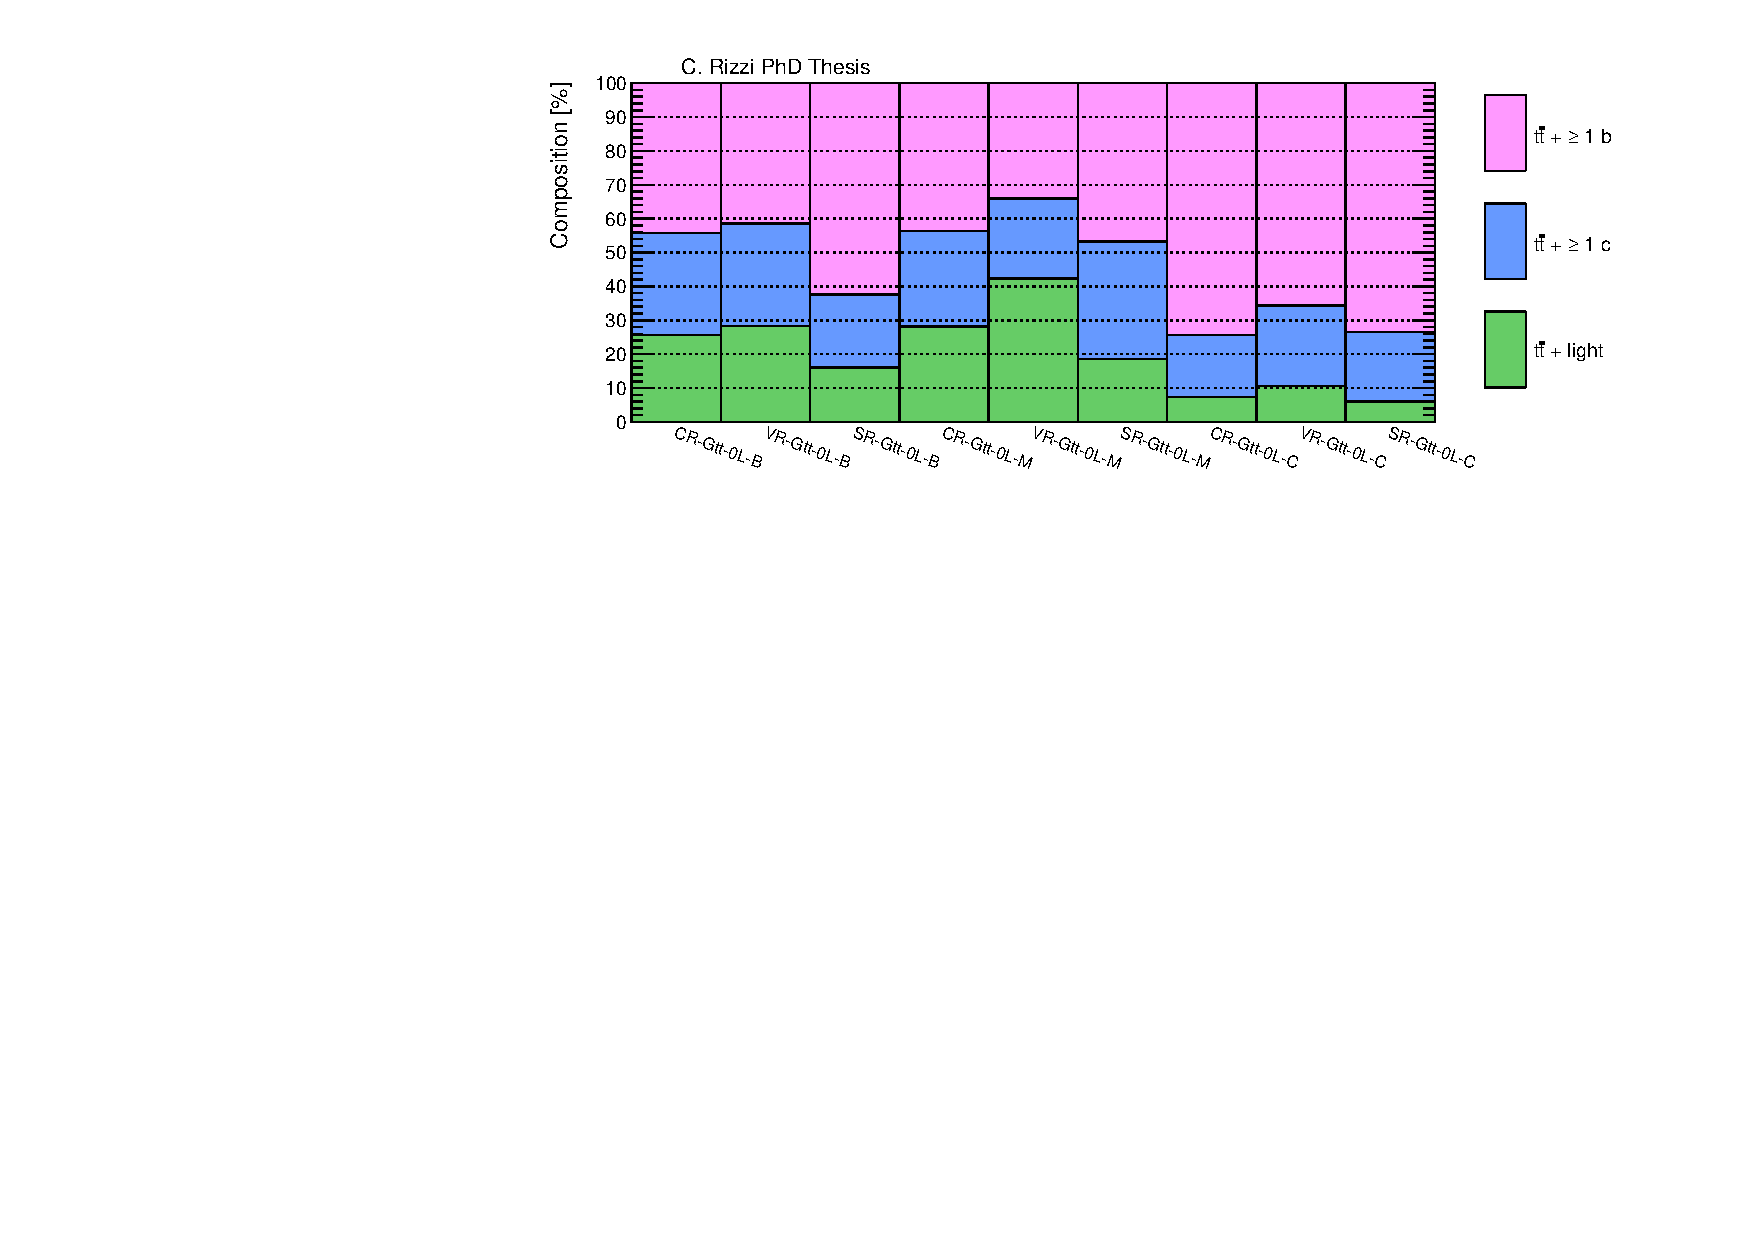
\includegraphics[width=\textwidth]{figures/strong_prod/comp_plots/Gtt_0L_HF.pdf}
\caption{Heavy-flavour composition in the \ttbar background in Gtt-0L regions.}
	\label{fig:HFcomp_Gtt0L}
\end{figure}

\begin{figure}[htbp]
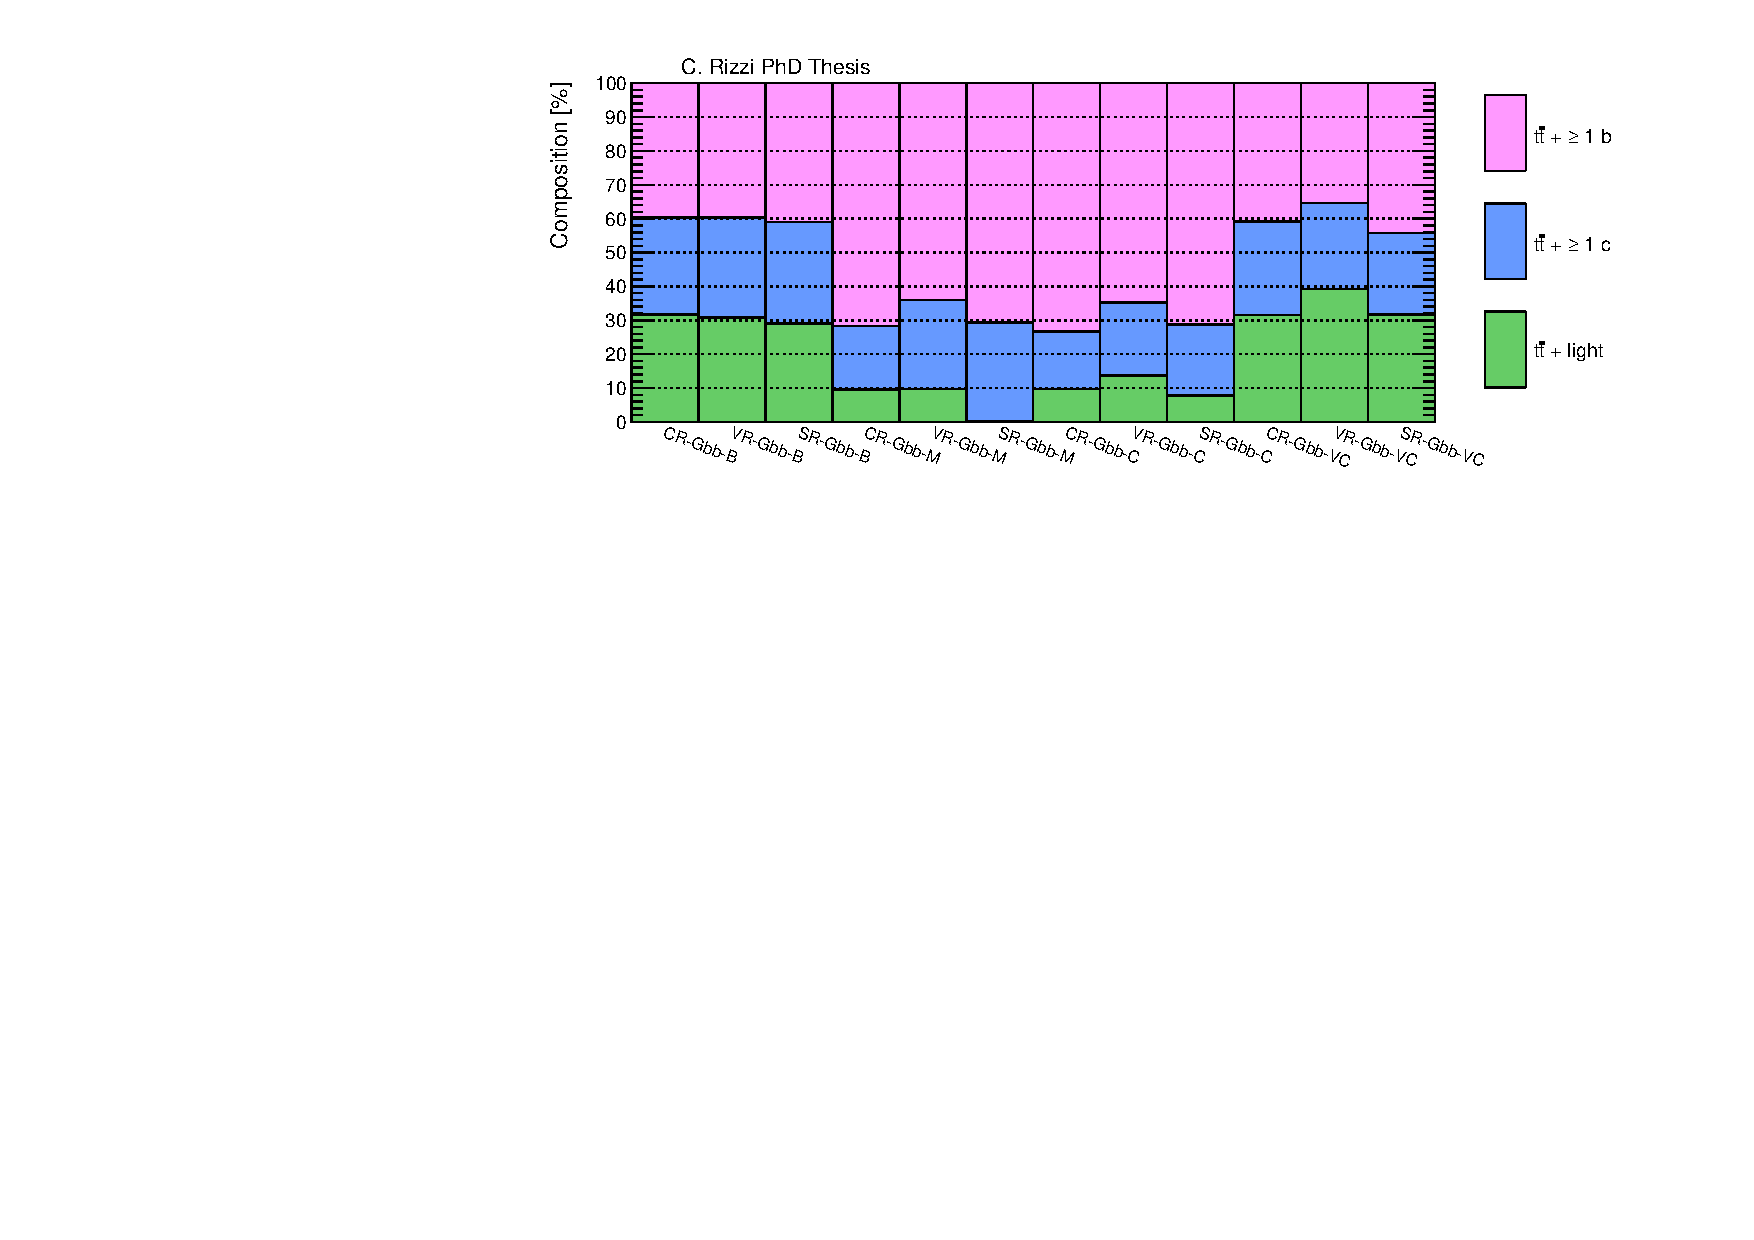
\includegraphics[width=\textwidth]{figures/strong_prod/comp_plots/Gbb_HF.pdf}
\caption{Heavy-flavour composition in the \ttbar background in Gbb regions.}
	\label{fig:HFcomp_Gbb}
\end{figure}

%%%%%

%\afterpage{\clearpage}
\FloatBarrier

\section{Multi-bin analysis regions}
\label{sec:strong:multibin}
In this section we describe the definition of the \glspl{sr}, \glspl{cr} and \glspl{vr} 
of the multi-bin analysis. 

\subsection{Signal regions}

The goal of the multi-bin strategy is to provide a set of regions each optimized for a different signal model 
but all mutually exclusive, so that they can be statistically combined to increase the exclusion power of the analysis.

Figure \ref{fig:strong:sig:jets_n} shows that the number of jets provides a good handle to separate 
between Gbb signal models, with lower number of jets, and Gtt signal models, where the number of jets is instead higher;
the Gtb model described in Section \ref{sec:strong:signalmodel} will have a number of jets intermediate between the Gtt and the Gtb case, 
as well as the mixed-\gls{br} case where one of the two produced gluinos decays to $b \bar{b} \ninoone$ and the other to 
$t \bar{t} \ninoone$.
Within a single decay topology, the variable that best discriminates between signals with different mass splitting between $\tilde{g}$ and
\ninoone is \meff: as shown in Figure \ref{fig:strong:sig:meff_incl}, signal models with larger mass splitting tend to have higher values 
of \meff, since the decay products are more boosted. 

These two variables are therefore used, together with the number of signal leptons, to categorize events into mutually exclusive regions. 
A schematic view of this categorization is given in Figure \ref{fig:multibin_scheme}, while the precise numerical values can be found 
in Tables \ref{tab:multibin_Hn}-\ref{tab:multibin_Ln}.
The naming convention for the multi-bin \glspl{sr} is the sequence of number of leptons, category for number of jets and category for \meff regime,
where the categories for \njet and \meff are labeled as "L" (low), "I" (intermediate) and "H" (high). So e.g. SR-0L-IL is the \gls{sr} in the 0-lepton channel with intermediate number of jets and low \meff. Low \njet regions are defined only in the 0-lepton channel, since they 
target Gbb signal models that do not produce final states with leptons. 

A dedicated \gls{sr} to target Gbb signal models where the gluino pair recoils against an \gls{isr} jet is designed following 
what is done for the cut-and-count analysis. 
Since the primary target of this \gls{isr} region are Gbb models with low mass splitting, its ideal phase space 
overlaps with that of the 0-lepton regions with low and intermediate \njet and low and intermediate \meff. 
This \gls{sr}-\gls{isr} relies on the selection of events where the leading jet is very energetic ($\pt > 400$ GeV),
 is not $b$-tagged and has a large angular separation with the \met in the event ($\dphilead > 2.9$). 
To allow orthogonality with the \gls{isr} regions, all the 0-lepton regions with low and intermediate \njet and low and intermediate \meff
are required to have either the leading jet $b$-tagged or $\dphilead < 2.9$. 

\begin{figure}[htbp]
	\subfigure[]{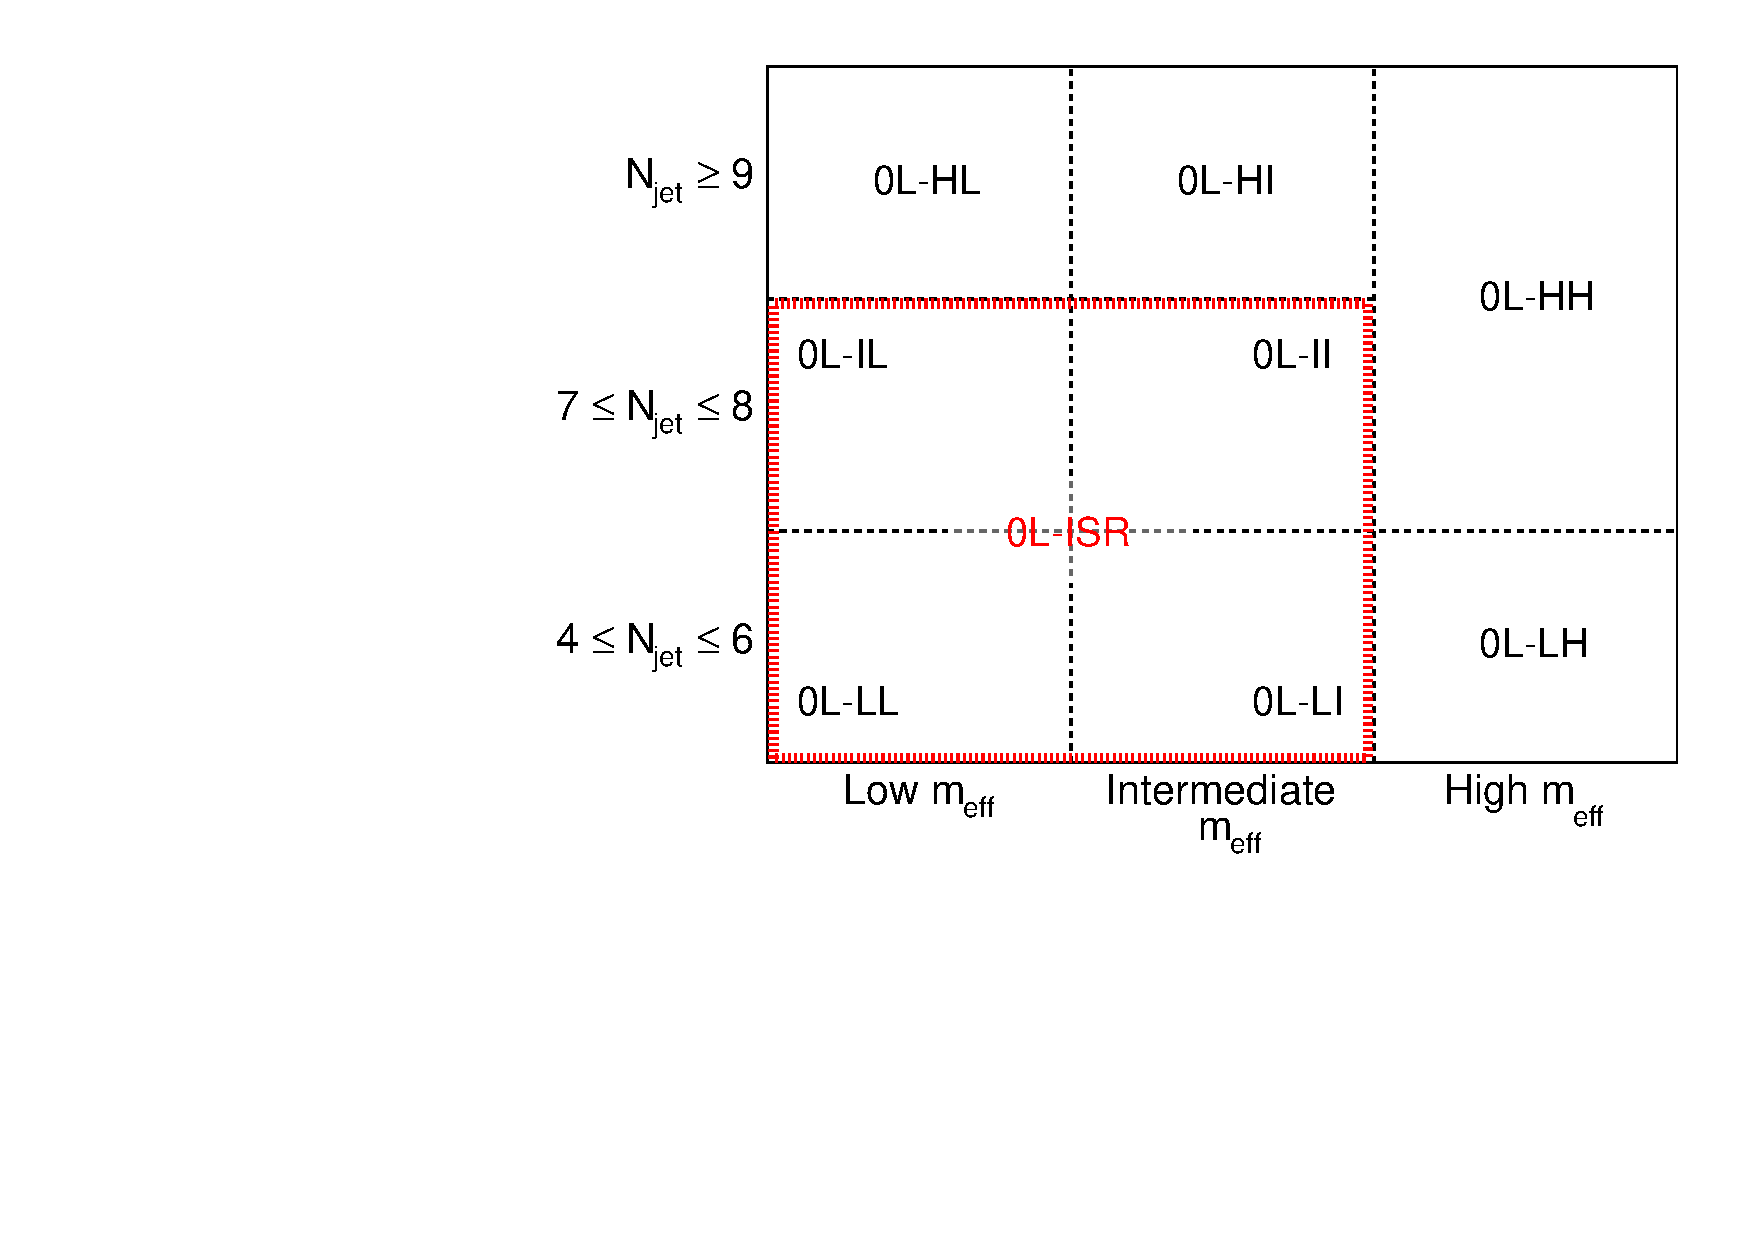
\includegraphics[width=0.49\linewidth]{figures/strong_prod/paper/selections/selections_0lep.pdf}\label{fig:multibin_scheme_0l}}
	\subfigure[]{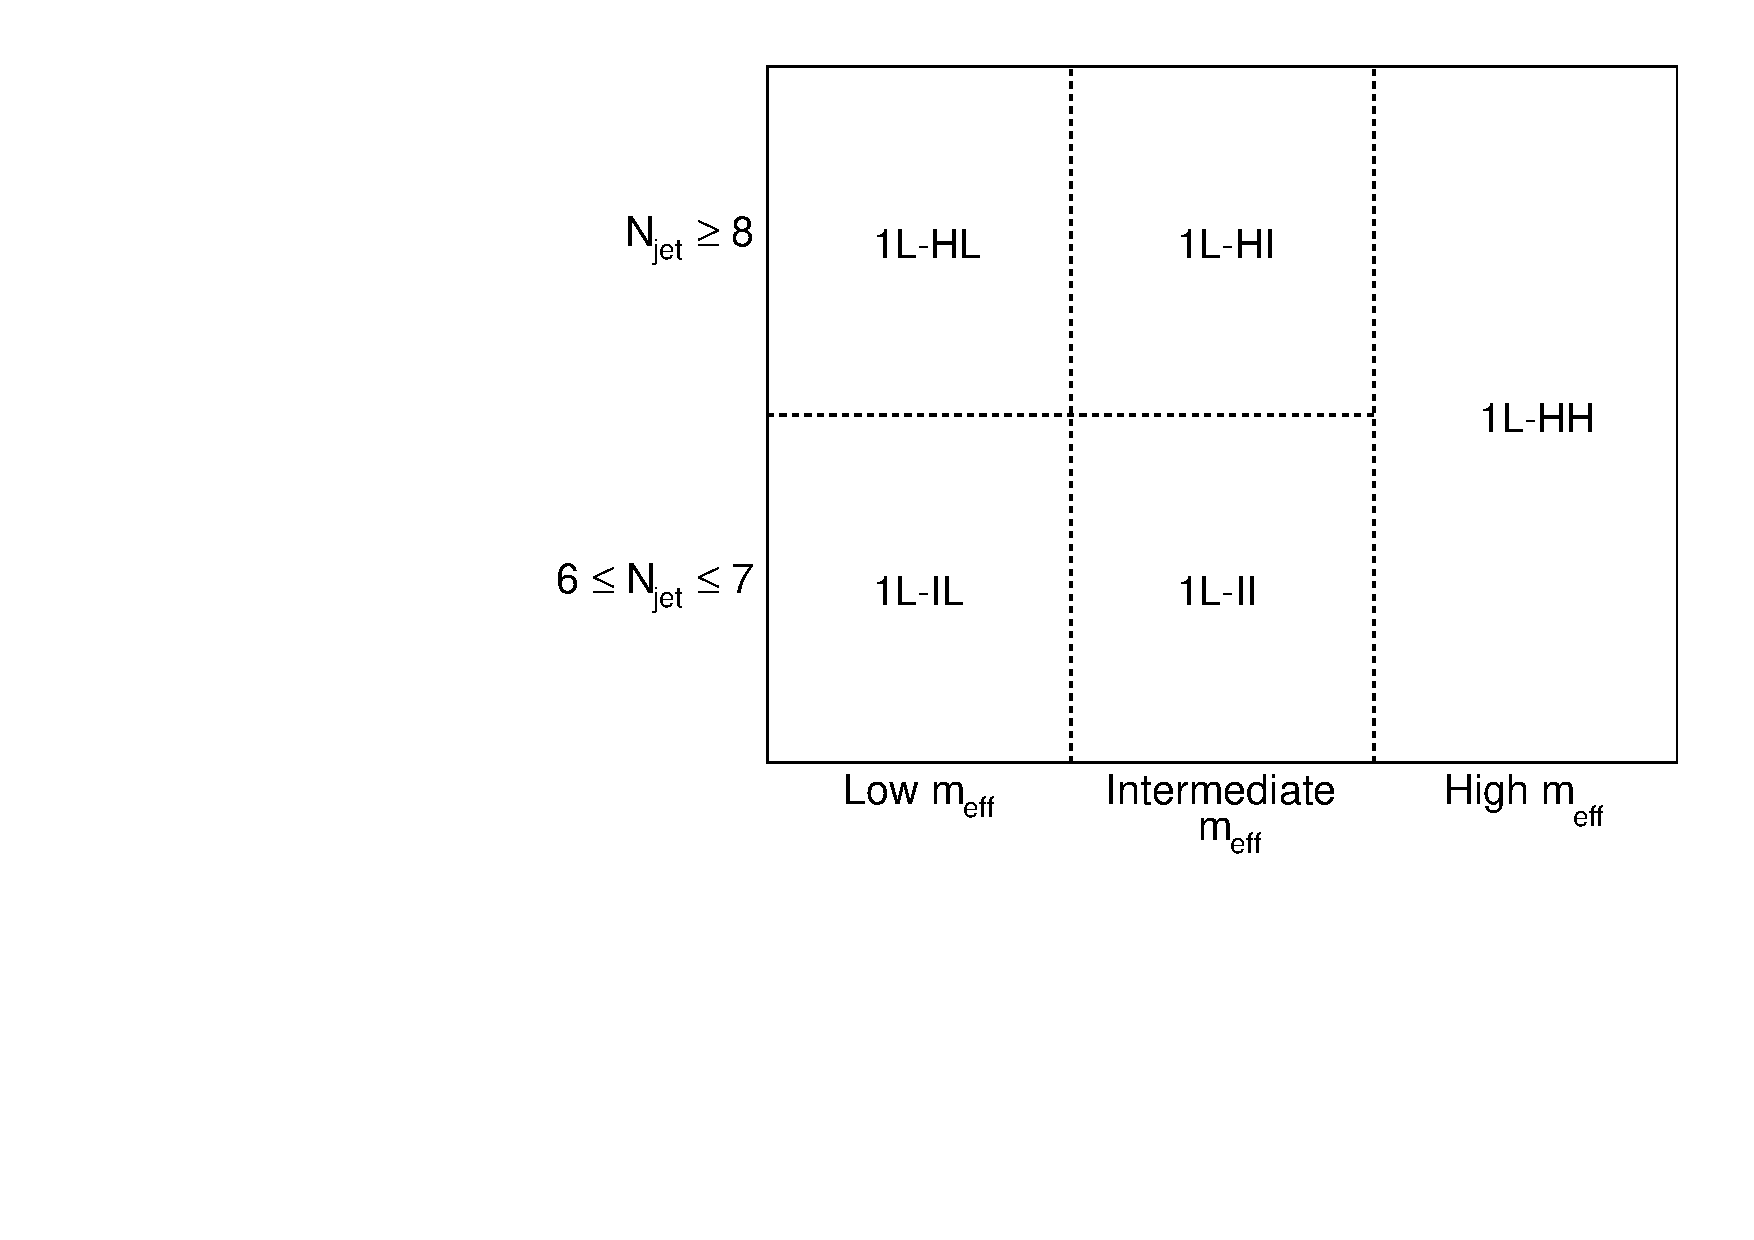
\includegraphics[width=0.49\linewidth]{figures/strong_prod/paper/selections/selections_1lep.pdf}\label{fig:multibin_scheme_1l}}
	\caption{Scheme of the multi-bin analysis for the \subref{fig:multibin_scheme_0l} 0-lepton 
	and \subref{fig:multibin_scheme_1l} 1-lepton regions. 
        The 0L-ISR region is represented with the broad red 
	dashed line in \subref{fig:multibin_scheme_0l}. 
      }
	\label{fig:multibin_scheme}
\end{figure}

In each of these mutually exclusive \gls{sr}, the selections on variables other than \njet, \nlep and \meff are optimized in a two-steps procedure:
\begin{enumerate}
\item First of all, in each region we define the set of selections that maximize the expected significance for a specific benchmark model, where the significance is defined as the number of standard deviations in a Gaussian that give the p-value obtained with Equation \ref{eq:binomexpp}. 
These selections have to satisfy the same criteria as for the cut-and-count \glspl{sr}, described in Section \ref{sec:strong:cutandcount}.
The benchmark models used to optimize each \gls{sr} are:
\begin{description}
\item[SR-0L-LL] Gbb, $m(\gluino) = 1.9$ TeV, $m(\ninoone) = 1.8$ TeV,
\item[SR-0L-LI] Gbb, $m(\gluino) = 1.9$ TeV, $m(\ninoone) = 600$ GeV,
\item[SR-0L-LH] Gbb, $m(\gluino) = 2.1$ TeV, $m(\ninoone) = 1$ GeV,
\item[SR-ISR]   Gbb, $m(\gluino) = 1.4$ TeV, $m(\ninoone) = 1.2$ TeV,

\item[SR-0L-IL] Gtt, $m(\gluino) = 1.9$ TeV, $m(\ninoone) = 1.4$ TeV,
\item[SR-0L-II] Gtt, $m(\gluino) = 1.9$ TeV, $m(\ninoone) = 600$ GeV,

\item[SR-1L-IL] Gtt, $m(\gluino) = 1.9$ TeV, $m(\ninoone) = 1.4$ TeV,
\item[SR-1L-II] Gtt, $m(\gluino) = 1.9$ TeV, $m(\ninoone) = 600$ GeV,

\item[SR-0L-HL] Gtt, $m(\gluino) = 1.9$ TeV, $m(\ninoone) = 1.4$ TeV,
\item[SR-0L-HI] Gtt, $m(\gluino) = 1.9$ TeV, $m(\ninoone) = 600$ GeV,
\item[SR-0L-HH] Gtt, $m(\gluino) = 2.1$ TeV, $m(\ninoone) = 1$ GeV,

\item[SR-1L-HL] Gtt, $m(\gluino) = 1.9$ TeV, $m(\ninoone) = 1.4$ TeV,
\item[SR-1L-HI] Gtt, $m(\gluino) = 1.9$ TeV, $m(\ninoone) = 600$ GeV,
\item[SR-1L-HH] Gtt, $m(\gluino) = 2.1$ TeV, $m(\ninoone) = 1$ GeV,

\end{description}


\item In a second step, we try to make the selections more uniform across all the regions, without penalizing the exclusion power. 
For each desired simplification of the selection, the exclusion contour is computed and compared to the original one obtained with the selections from the first step. If the simplification of the selections does not bring any significant loss in the exclusion sensitivity, the simplification is adopted. This is the case e.g. for the \mt selection, which takes the value of $>150$ GeV for all the 1-lepton \glspl{sr}.
\end{enumerate}



\subsection{Control regions and validation regions}

As in the case of the cut-and-count strategy, all the \glspl{cr} require at least one signal lepton. 
In the multi-bin strategy the corresponding 0L and 1L \glspl{sr} share the same \gls{cr}.
This choice is motivated by the observation that 0L and 1L \glspl{sr} in the multi-bin approach are 
kinematically closer than Gtt-0L and Gtt-1L regions targeting similar signal topology, 
and also by the need to have \glspl{cr} that are either mutually exclusive or completely overlapping to 
allow the simultaneous inclusion of all the regions in the fit. 

Also in the multi-bin approach, the \glspl{cr} rely on an inverted selection on \mt to maintain orthogonality with 
the corresponding \glspl{sr}-1L. The requirement on the number of jets is the same as in the \glspl{sr}-1L, while the 
\glspl{sr}-0L require one extra jet. Selections on other variables are relaxed to allow enough expected \ttbar events in 
each \gls{cr}.
The extrapolation from the \gls{cr} to each \gls{sr} is tested with a dedicated \gls{vr}. 
The \glspl{vr}-0L are orthogonal to the corresponding \glspl{sr} through inversion of the \mtb, \meff or \met selection;
the \glspl{vr}-1L have the same \mt selection as the \glspl{sr} and are orthogonal to those thanks to
an inverted \mtb selection.

To allow enough statistics in all the \glspl{vr}, two of them (VR-1L-HI and VR-1L-HL) are not orthogonal.
This does not constitute a problem since the \glspl{vr}
are not included in the statistical fit and 
the overlap has been quantified to be around 15\% of the events in these \glspl{vr}; therefore 
the validity of the conclusions is not compromised. 

%\clearpage

\begin{landscape}
	\begin{table}[htbp]
   		\centering
        		\renewcommand{\arraystretch}{1.5}
        		\begin{tabular}{c c c c c c c c c c}
        			\toprule
			\multicolumn{10}{c}{\textbf{ High-$\njet$ regions}}\\
			\multicolumn{10}{c}{Criteria common to all regions: $\nbjet \geq 3$, ${\pt}^\mathrm{jet} > 30$~GeV } \\
			\midrule 
			Targeted kinematics  & Type & \nlep & $\dphimin$ & $\mt$ & \njet & $\mtb$ & $\mjsum$ & $\met$ & $\meff$  \\
			\midrule
			\multirow{5}{*}{\begin{minipage}{3cm}\centering High-\meff\ \\ (HH) \\ (Large \msplit) \end{minipage}} 
			& SR-0L 	& $= 0$  		& $>0.4$ 		& $-$ 		& $\ge 7$		& $>100 $ 			& $>200$ 	& $> 400 $ 				& $> 2500$ \\ 
			& SR-1L 	& $\ge 1$  	& $-$		& $> 150 $ 	& $\ge 6$		& $> 120$ 			& $>200$ 	& $> 500 $ 				& $> 2300$ \\ 
			& CR 	& $\ge 1$  	& $-$ 		& $< 150$ 	& $\ge 6$		& $> 60 $ 				& $>150$ 	& $> 300 $ 				& $> 2100$ \\ 
			& VR-0L 	& $= 0$  		& $>0.4$ 		& $-$ 		& $\ge 7$		& $<100$ if $\met>300$ 	& $-$ 	& $< 300 $ if $\mtb > 100$ 	& $> 2100$ \\
			& VR-1L 	& $\ge 1$  	& $-$ 		& $> 150$ 	& $\ge 6$		& $<140$ if $\meff>2300$	& $-$ 	& $< 500$  				& $> 2100$ \\
			\midrule
			\multirow{5}{*}{\begin{minipage}{3cm}\centering Intermediate-\meff\ \\ (HI) \\ (Intermediate \msplit) \end{minipage}} 
			& SR-0L 	& $= 0$  		& $>0.4$ 		& $-$ 		& $\ge 9$		& $> 140$ 			& $>150$ 	& $> 300 $ 				& $[1800, 2500]$ \\ 
			& SR-1L 	& $\ge 1$  	& $-$		& $> 150 $ 	& $\ge 8$		& $> 140$ 			& $>150$ 	& $> 300 $ 				& $[1800, 2300]$ \\ 
			& CR 	& $\ge 1$  	& $-$ 		& $< 150$ 	& $\ge 8$		& $> 60$ 				& $>150$ 	& $> 200 $ 				& $[1700, 2100]$ \\ 
			& VR-0L 	& $= 0$  		& $>0.4$ 		& $-$ 		& $\ge 9$		& $<140$ if $\met>300$ 	& $-$ 	& $< 300 $ if $\mtb > 140$ 	& $[1650, 2100]$ \\
			& VR-1L 	& $\ge 1$  	& $-$ 		& $> 150$ 	& $\ge 8$		& $<140$ if $\met>300$	& $-$ 	& $< 300 $ if $\mtb > 140$	& $[1600, 2100]$ \\
			\midrule
			\multirow{5}{*}{\begin{minipage}{3cm}\centering Low-\meff\ \\ (HL) \\ (Small \msplit) \end{minipage}} 
			& SR-0L 	& $= 0$  		& $>0.4$ 		& $-$ 		& $\ge 9$		& $> 140$ 			& $-$ 	& $> 300 $ 				& $[900, 1800]$ \\ 
			& SR-1L 	& $\ge 1$  	& $-$		& $> 150 $ 	& $\ge 8$		& $> 140$ 			& $-$ 	& $> 300 $ 				& $[900, 1800]$ \\ 
			& CR 	& $\ge 1$  	& $-$ 		& $< 150$ 	& $\ge 8$		& $> 130$ 			& $-$ 	& $> 250 $ 				& $[900, 1700]$ \\ 
			& VR-0L 	& $= 0$  		& $>0.4$ 		& $-$ 		& $\ge 9$		& $<140$				& $-$ 	& $> 300 $ 				& $[900, 1650]$ \\
			& VR-1L 	& $\ge 1$  	& $-$ 		& $> 150$ 	& $\ge 8$		& $<140$				& $-$ 	& $> 225 $			 	& $[900, 1650]$ \\
      			\bottomrule
    		\end{tabular}
    		 \caption{Definition of the high-$\njet$ SRs, CRs and VRs of the multi-bin analysis. All kinematic variables are
                          expressed in \gev\ except $\dphimin$, which is in radians.  Table from Ref. \cite{Aaboud:2017hrg}.}
                        \label{tab:multibin_Hn}
 	\end{table}
\end{landscape}

%\clearpage

\begin{landscape}
	\begin{table}[htbp]
		\small
   		\centering
        		\renewcommand{\arraystretch}{1.5}
                        \label{tab:multibin_In}
        		\begin{tabular}{c c c c c c c c c c c}
        			\toprule
			\multicolumn{11}{c}{\textbf{ Intermediate-$\njet$ regions}}\\
			\multicolumn{11}{c}{Criteria common to all regions: $\nbjet \geq 3$, ${\pt}^\mathrm{jet} > 30$~GeV } \\
			\midrule 
			Targeted kinematics  & Type & $N_\mathrm{lepton}$ & $\dphimin$ & $\mt$ & $\njet$ & $\leadjet = b$ or $\dphilead \leq 2.9$ & $\mtb$ & $\mjsum$  & $\met$ & $\meff$  \\
			\midrule
			\multirow{5}{*}{\begin{minipage}{3cm}\centering Intermediate-\meff\ \\ (II) \\ (Intermediate \msplit) \end{minipage}} 
			& SR-0L 	& $= 0$  		& $>0.4$ 		& $-$ 		& $[7,8]$		& \cmark		& $> 140 $ 			& $>150$ 		& $> 300 $ 				& $[1600,2500]$ \\ 
			& SR-1L 	& $\ge 1$  	& $-$		& $> 150 $ 	& $[6,7]$		& $-$ 		& $> 140$ 			& $>150$ 		& $> 300 $ 				& $[1600,2300]$ \\ 
			& CR 	& $\ge 1$  	& $-$ 		& $< 150$ 	& $[6,7]$		& \cmark 		& $> 110 $ 			& $>150$ 		& $> 200 $ 				& $[1600,2100]$ \\ 
			& VR-0L 	& $= 0$  		& $>0.4$ 		& $-$ 		& $[7,8]$		& \cmark		& $<140$ 				& $-$ 		& $> 300 $ 				& $[1450,2000]$ \\
			& VR-1L 	& $\ge 1$  	& $-$ 		& $> 150$ 	& $[6,7]$		& $-$		& $<140$				& $-$ 		& $> 225 $  				& $[1450,2000]$ \\
			\midrule
			\multirow{5}{*}{\begin{minipage}{3cm}\centering Low-\meff\ \\ (IL) \\ (Low \msplit) \end{minipage}} 
			& SR-0L 	& $= 0$  		& $>0.4$ 		& $-$ 		& $[7,8]$		& \cmark		& $> 140 $ 			& $-$ 		& $> 300 $ 				& $[800,1600]$ \\ 
			& SR-1L 	& $\ge 1$  	& $-$		& $> 150 $ 	& $[6,7]$		& $-$ 		& $> 140$ 			& $-$ 		& $> 300 $ 				& $[800,1600]$ \\ 
			& CR 	& $\ge 1$  	& $-$ 		& $< 150$ 	& $[6,7]$		& \cmark 		& $> 130 $ 			& $-$ 		& $> 300 $ 				& $[800,1600]$ \\ 
			& VR-0L 	& $= 0$  		& $>0.4$ 		& $-$ 		& $[7,8]$		& \cmark		& $<140$ 				& $-$ 		& $> 300 $ 				& $[800,1450]$ \\
			& VR-1L 	& $\ge 1$  	& $-$ 		& $> 150$ 	& $[6,7]$		& $-$		& $<140$				& $-$ 		& $> 300 $  				& $[800,1450]$ \\
      			\bottomrule
    		\end{tabular}
    \caption{Definition of the intermediate-$\njet$ SRs, CRs and VRs of the multi-bin analysis. All kinematic variables are
                          expressed in \gev\ except $\dphimin$, which is in radians. The $\leadjet = b$  requirement specifies that 
                          the leading jet is $b$-tagged.  Table from Ref. \cite{Aaboud:2017hrg}.}
 	\end{table}
\end{landscape}

%\clearpage

\begin{landscape}
	\begin{table}[htbp]
   		\centering
        		\renewcommand{\arraystretch}{1.1}	
        		\begin{tabular}{c c c c c c c c c c c }
        			\toprule
			\multicolumn{11}{c}{\textbf{ Low-$\njet$ regions}}\\
			\multicolumn{11}{c}{Criteria common to all regions: $\nbjet \geq 3$, ${\pt}^\mathrm{jet} > 30$~GeV } \\
			\midrule 
			Targeted kinematics  & Type & $N_\mathrm{lepton}$ & $\dphimin$ & $\mt$ & $\njet$ & $\leadjet = b$ or $\dphilead \leq 2.9$ & $\pt^{\fourthjet}$ & $\mtb$ & $\met$ & $\meff$  \\
			\midrule
			\multirow{3}{*}{\begin{minipage}{3cm}\centering High-\meff\ \\ (LH) \\ (Large \msplit) \end{minipage}} 
			& SR 	& $= 0$  		& $>0.4$ 		& $-$ 		& $[4,6]$		& $-$		& $>90$					& $-$ 			& $> 300 $ 				& $> 2400$ \\ 
			& CR 	& $\ge 1$  	& $-$ 		& $< 150$ 	& $[4,5]$		& $-$ 	 	& -						& $-$ 			& $> 200 $ 				& $> 2100$ \\ 
			& VR 	& $= 0$  		& $>0.4$ 		& $-$ 		& $[4,6]$		& $-$ 		& $>90$ if $\met < 300$		& $-$			& $> 200 $ 				& $[2000,2400]$ \\
			\midrule
			\multirow{3}{*}{\begin{minipage}{3cm}\centering Intermediate-\meff\ \\ (LI) \\ (Intermediate \msplit) \end{minipage}} 
			& SR 	& $= 0$  		& $>0.4$ 		& $-$ 		& $[4,6]$		& \cmark		& $>90$				& $>140$ 		& $> 350 $ 				& $[1400,2400]$ \\ 
			& CR 	& $\ge 1$  	& $-$ 		& $< 150$ 	& $[4,5]$		& \cmark 	 	& $>70$				& $-$ 		& $> 300 $ 				& $[1400,2000]$ \\ 
			& VR 	& $= 0$  		& $>0.4$ 		& $-$ 		& $[4,6]$		& \cmark		& $>90$				& $<140$ 		& $> 300 $ 				& $[1250,1800]$ \\
			\midrule
			\multirow{3}{*}{\begin{minipage}{3cm}\centering Low-\meff\ \\ (LL) \\ (Low \msplit) \end{minipage}} 
			& SR 	& $= 0$  		& $>0.4$ 		& $-$ 		& $[4,6]$		& \cmark		& $>90$				& $>140$ 		& $> 350 $ 				& $[800,1400]$ \\ 
			& CR 	& $\ge 1$  	& $-$ 		& $< 150$ 	& $[4,5]$		& \cmark 	 	& $>70$				& $-$ 		& $> 300 $ 				& $[800,1400]$ \\ 
			& VR 	& $= 0$  		& $>0.4$ 		& $-$ 		& $[4,6]$		& \cmark		& $>90$				& $<140$ 		& $> 300 $ 				& $[800,1250]$ \\
      			\bottomrule
    		\end{tabular}
		
		\par\medskip
		
    		\begin{tabular}{K{1.5cm} K{1.5cm} K{1.5cm} K{1.5cm} K{1.5cm} K{1.5cm} K{1.5cm} K{1.5cm} }
        			\toprule
			\multicolumn{8}{c}{\textbf{ ISR regions}}\\
			\multicolumn{8}{c}{Criteria common to all regions: $\nbjet \geq 3$, $\dphilead > 2.9$, ${\pt}^\leadjet > 400$~\gev, ${\pt}^\mathrm{jet} > 30$~GeV, $\leadjet \neq b$} \\
			\midrule 
			Type & $N_\mathrm{lepton}$ & $\dphimin$ & $\mt$ & $\njet$ & $\mtb$ & $\met$ & $\meff$  \\
			\midrule
			SR 	& $= 0$  		& $>0.4$ 		& $-$ 		& $[4,8]$		& $>100$ 			& $> 600 $ 				& $<2200$ \\ 
			CR 	& $\ge 1$  	& $-$ 		& $< 150$ 	& $[4,7]$		& $-$ 			& $> 400 $ 				& $<2000$ \\ 
			VR 	& $= 0$  		& $>0.4$ 		& $-$ 		& $[4,8]$		& $>100$ 			& $[250,600] $ 				& $<2000$ \\
      			\bottomrule
    		\end{tabular}
\caption{Definition of the low-$\njet$ and ISR SRs, CRs and VRs of the multi-bin analysis. All kinematic variables are
                          expressed in \gev\ except $\dphimin$, which is
                          in radians. The $\leadjet = b$ ($\leadjet \neq b$) requirement specifies that 
                          the leading jet is (not) $b$-tagged.  Table from Ref. \cite{Aaboud:2017hrg}.}
                        \label{tab:multibin_Ln}
                        %\label{tab:multibin_ISR}	
 	\end{table}
\end{landscape}

%\afterpage{\clearpage}


\subsection{Background composition}

The pre-fit background composition in the the multi-bin analysis regions is shown in Figures \ref{fig:bkgcomp_Hnj}-\ref{fig:bkgcomp_Lnj}, 
for the regions with high, intermediate and low number of jets.
Just like in the cut-and-count analysis regions, \ttbar is the dominant background in all the \glspl{sr}, 
and all the \glspl{cr} and the \glspl{vr} have a high \ttbar purity.

Figures \ref{fig:ttcomp_Hnj} to \ref{fig:ttcomp_Lnj} show the decay type of the \ttbar background for the regions with high, intermediate and low number of jets, classified as described in Section \ref{sec:susy_general:ttbar}.
As already noticed when discussing the cut-and-count regions, the \glspl{sr}-1L and \glspl{vr}-1L are dominated by 
dilepton \ttbar since the $\mt > 150$ GeV selection suppresses single-lepton \ttbar background, which is instead dominant in the \glspl{cr} and in 
the 0-lepton regions. In the case of \glspl{sr}-0L and \glspl{vr}-0L the selected \ttbar events are mostly the ones where one 
of the top quarks decays hadronically and the other one to a $\tau$-lepton.



The classification of the \ttbar background based on the flavour of the jets associated to the 
\ttbar production, as described in Section \ref{sec:susy_general:ttbar}, is shown in Figures 
\ref{fig:HFcomp_Hnj}-\ref{fig:HFcomp_Lnj}.
%Thanks to adopting the same selection on the number of $b$-jets in \gls{cr}, \gls{sr} and \glspl{vr} 
%of the same region type, composition is similar in corresponding regions, even if the fraction of 
%\tthf is sometimes higher in the \glspl{sr}, especially in the case of Gtt-1L regions. 

\begin{figure}[htbp]
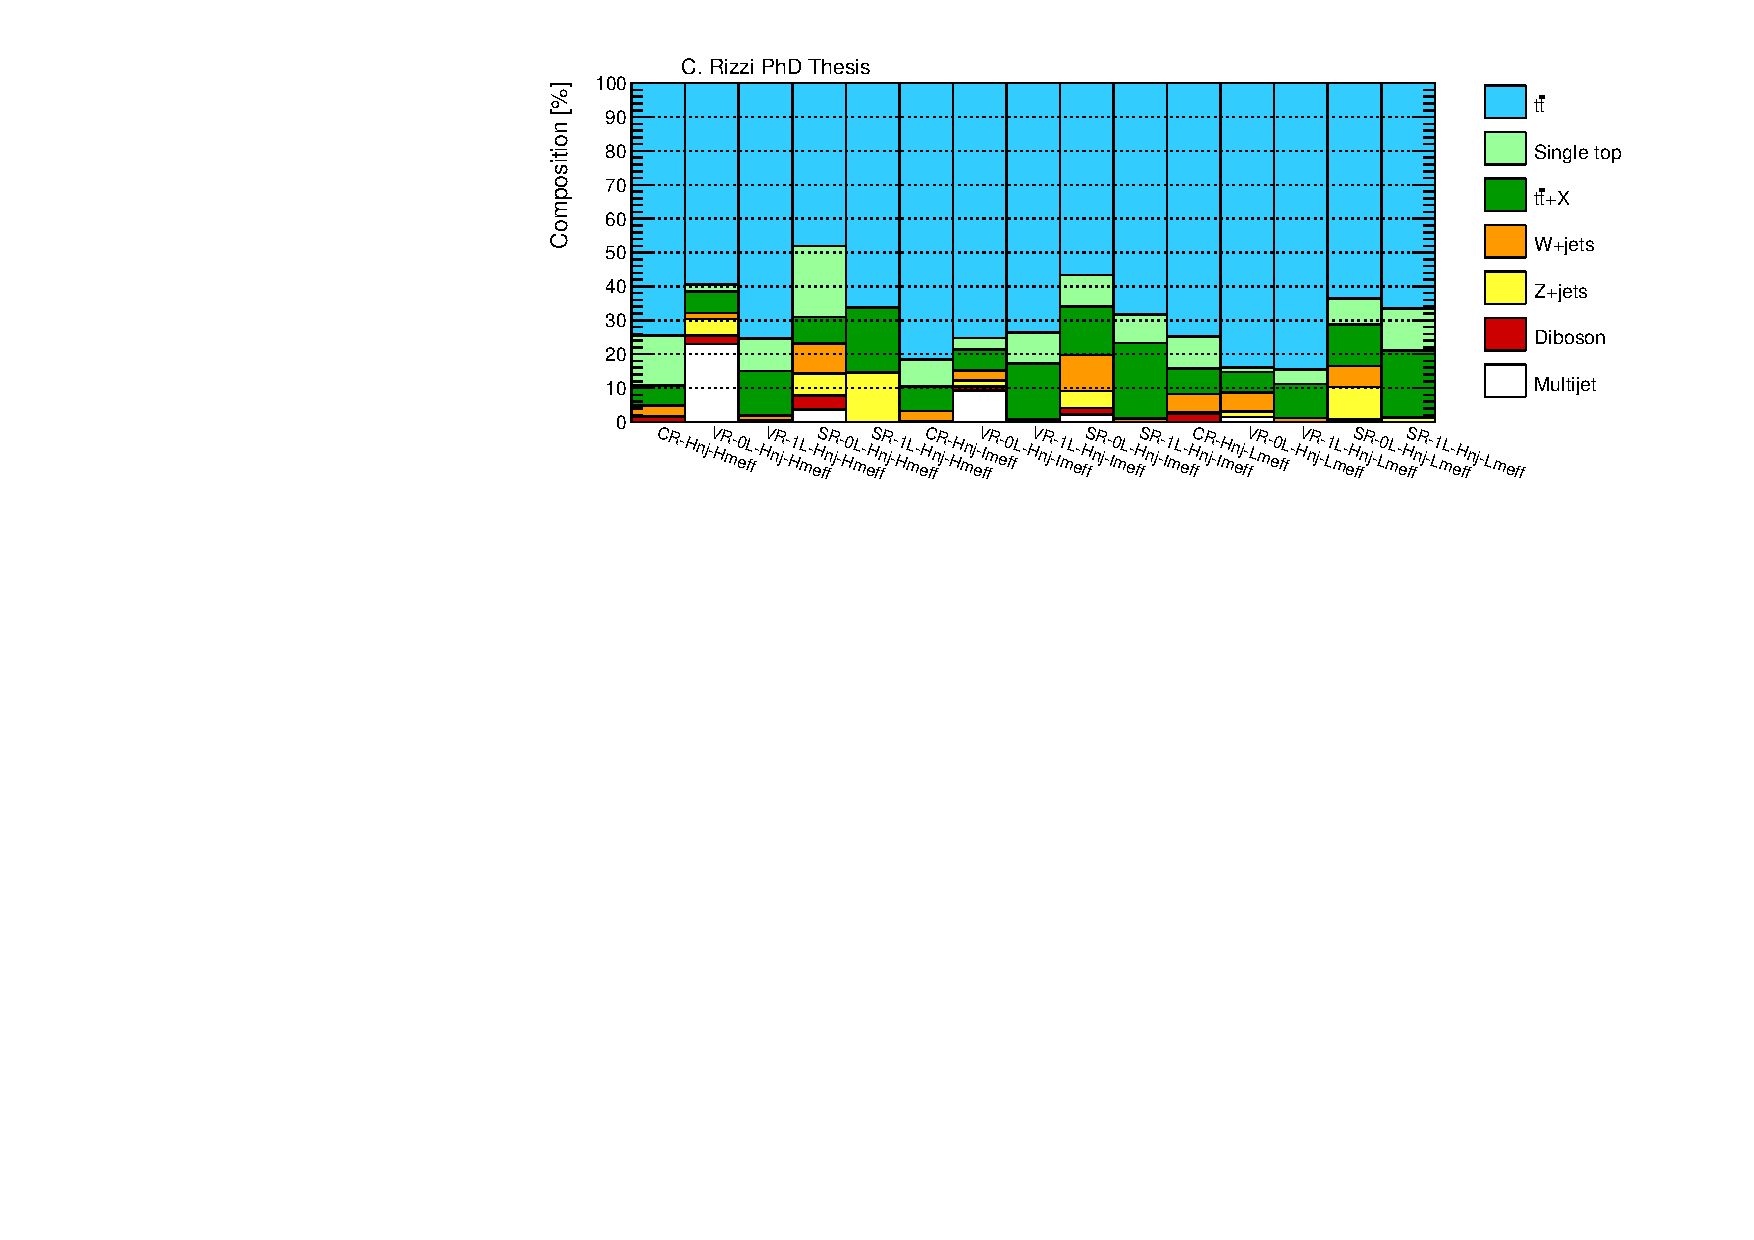
\includegraphics[width=\textwidth]{figures/strong_prod/comp_plots/Hnj_bkg.pdf}
\caption{Background composition in the the multi-bin regions with high number of jets.}
	\label{fig:bkgcomp_Hnj}
\end{figure}

\begin{figure}[htbp]
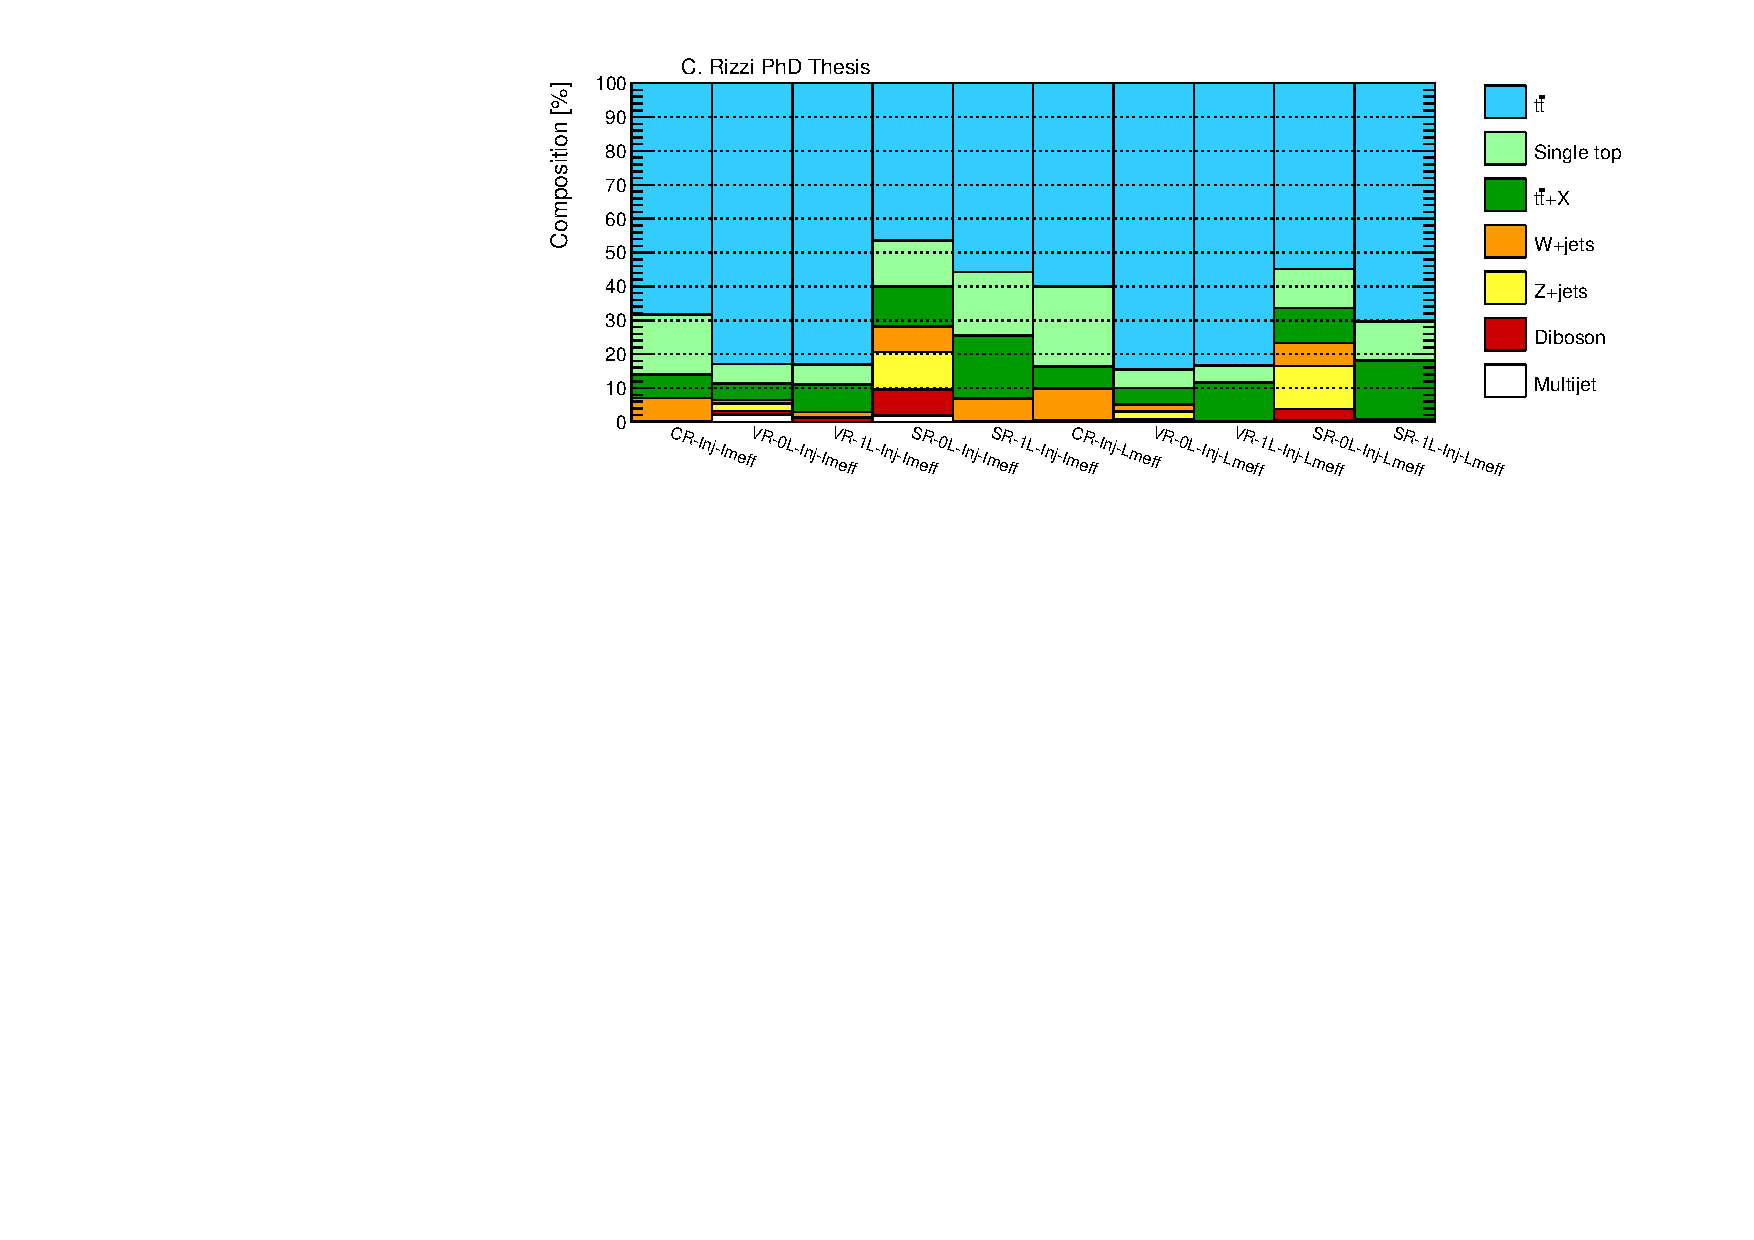
\includegraphics[width=\textwidth]{figures/strong_prod/comp_plots/Inj_bkg.pdf}
\caption{Background composition in the the multi-bin regions with intermediate number of jets.}
	\label{fig:bkgcomp_Inj}
\end{figure}

\begin{figure}[htbp]
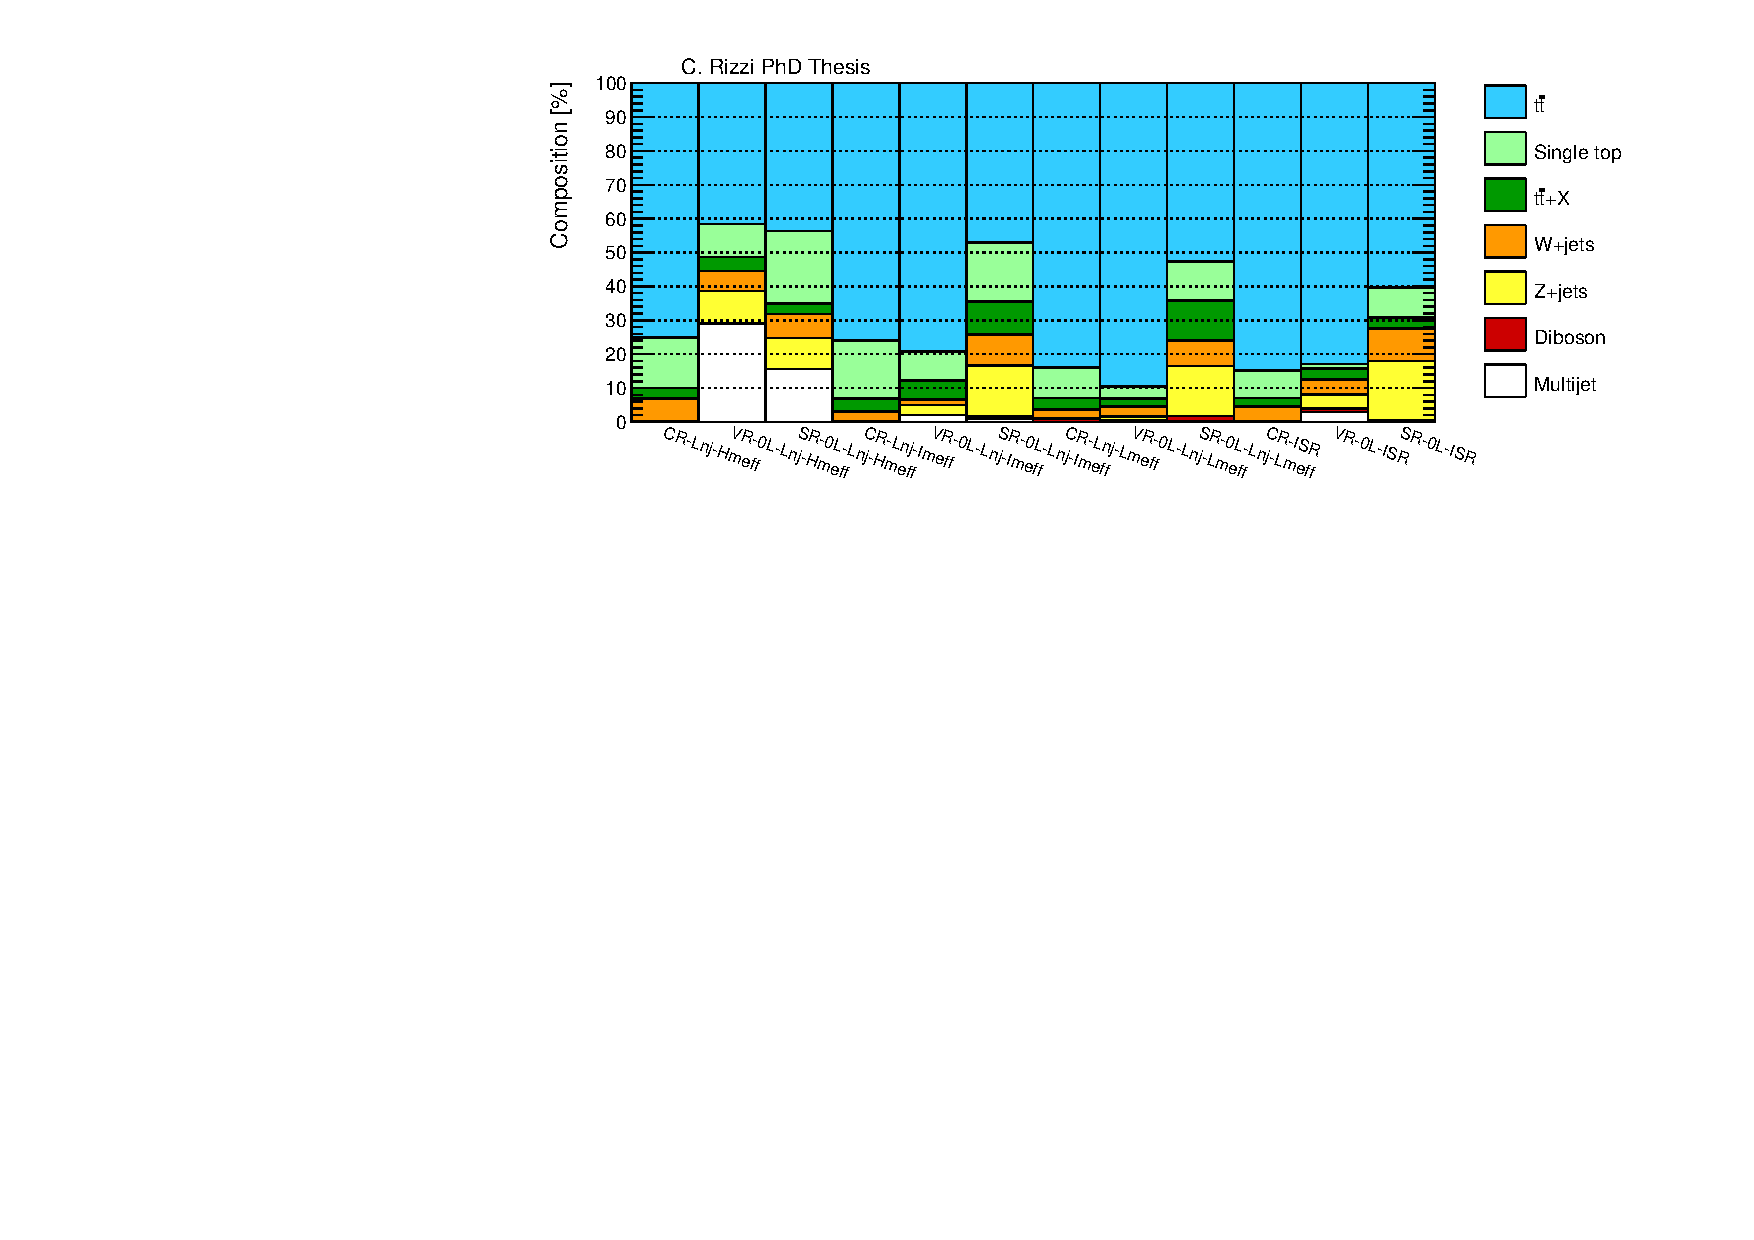
\includegraphics[width=\textwidth]{figures/strong_prod/comp_plots/Lnj_bkg.pdf}
\caption{Background composition in the the multi-bin regions with low number of jets.}
	\label{fig:bkgcomp_Lnj}
\end{figure}



\begin{figure}[htbp]
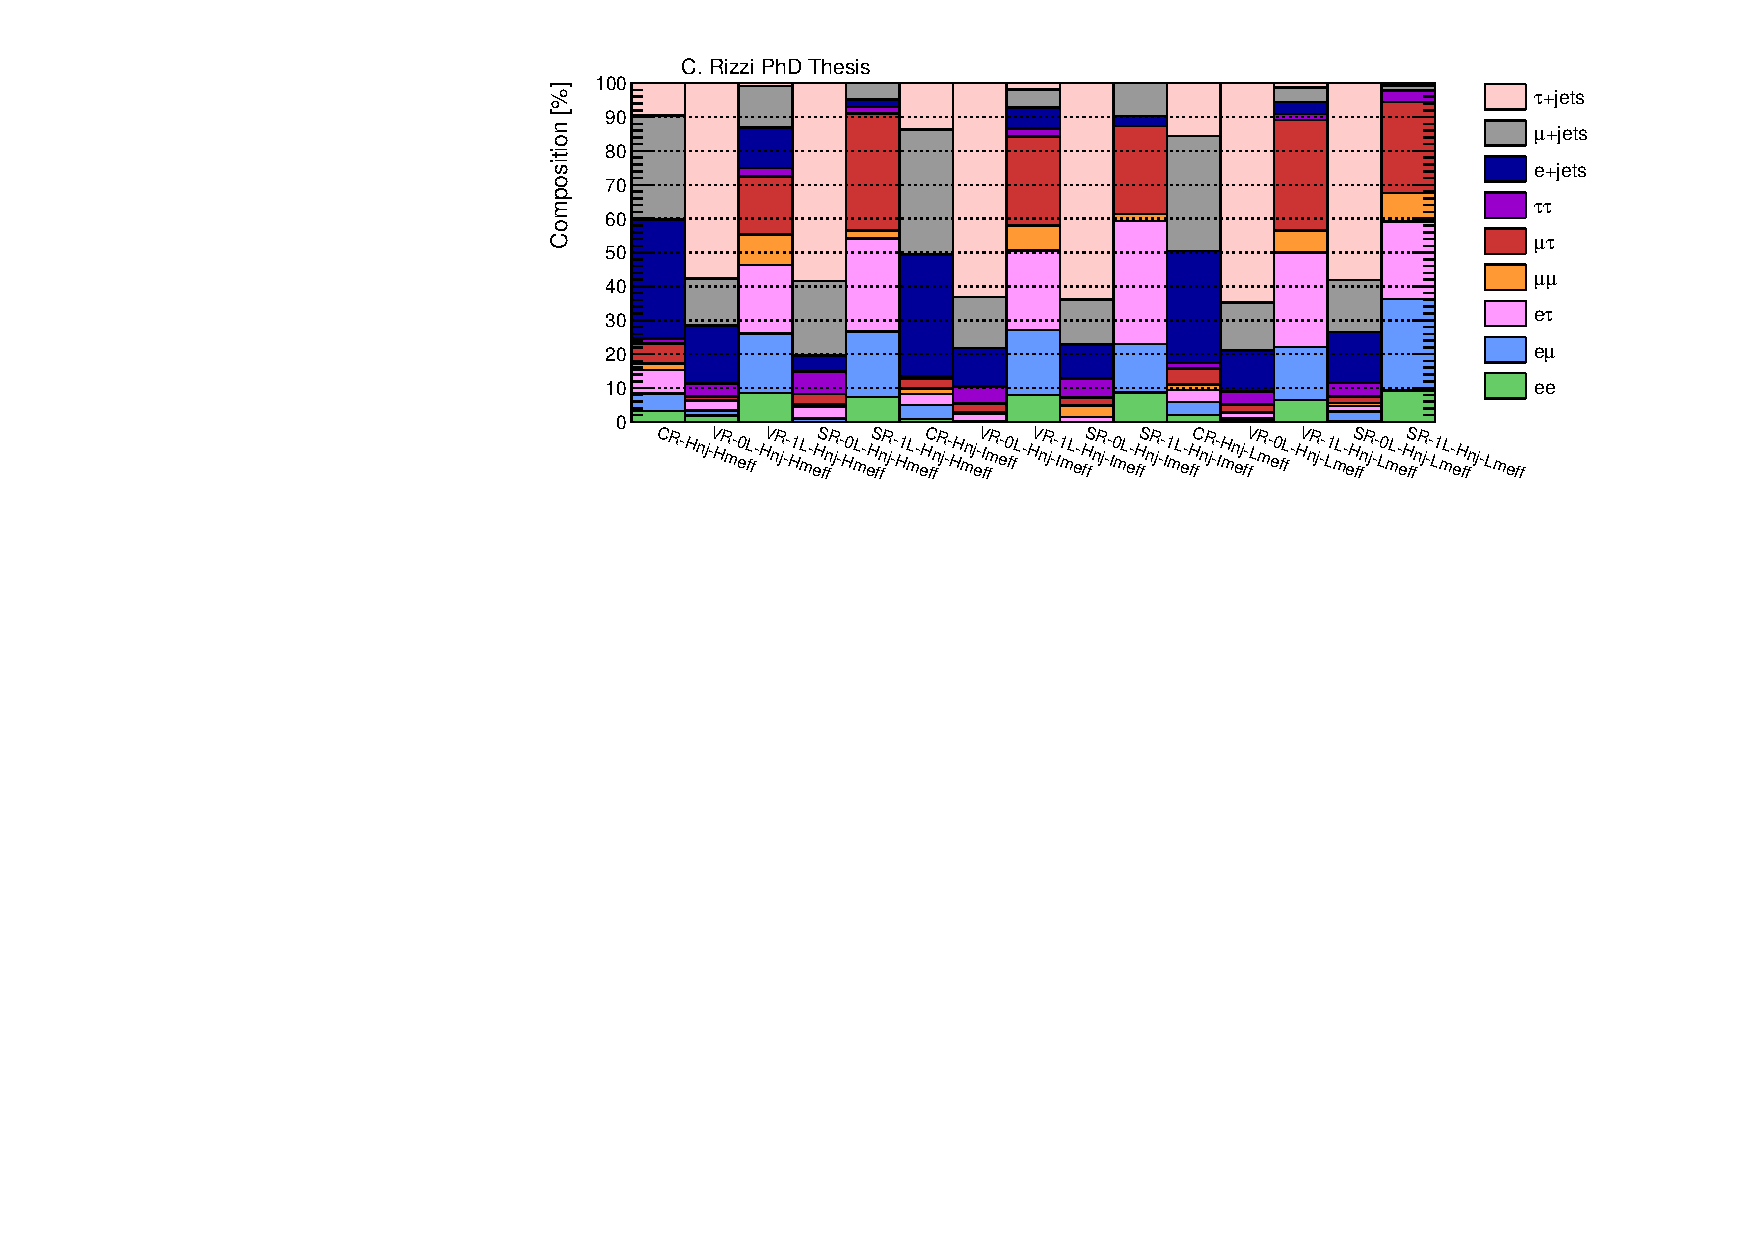
\includegraphics[width=\textwidth]{figures/strong_prod/comp_plots/Hnj_tt.pdf}
\caption{Decay mode of the \ttbar background in the the multi-bin regions with high number of jets.}
	\label{fig:ttcomp_Hnj}
\end{figure}

\begin{figure}[htbp]
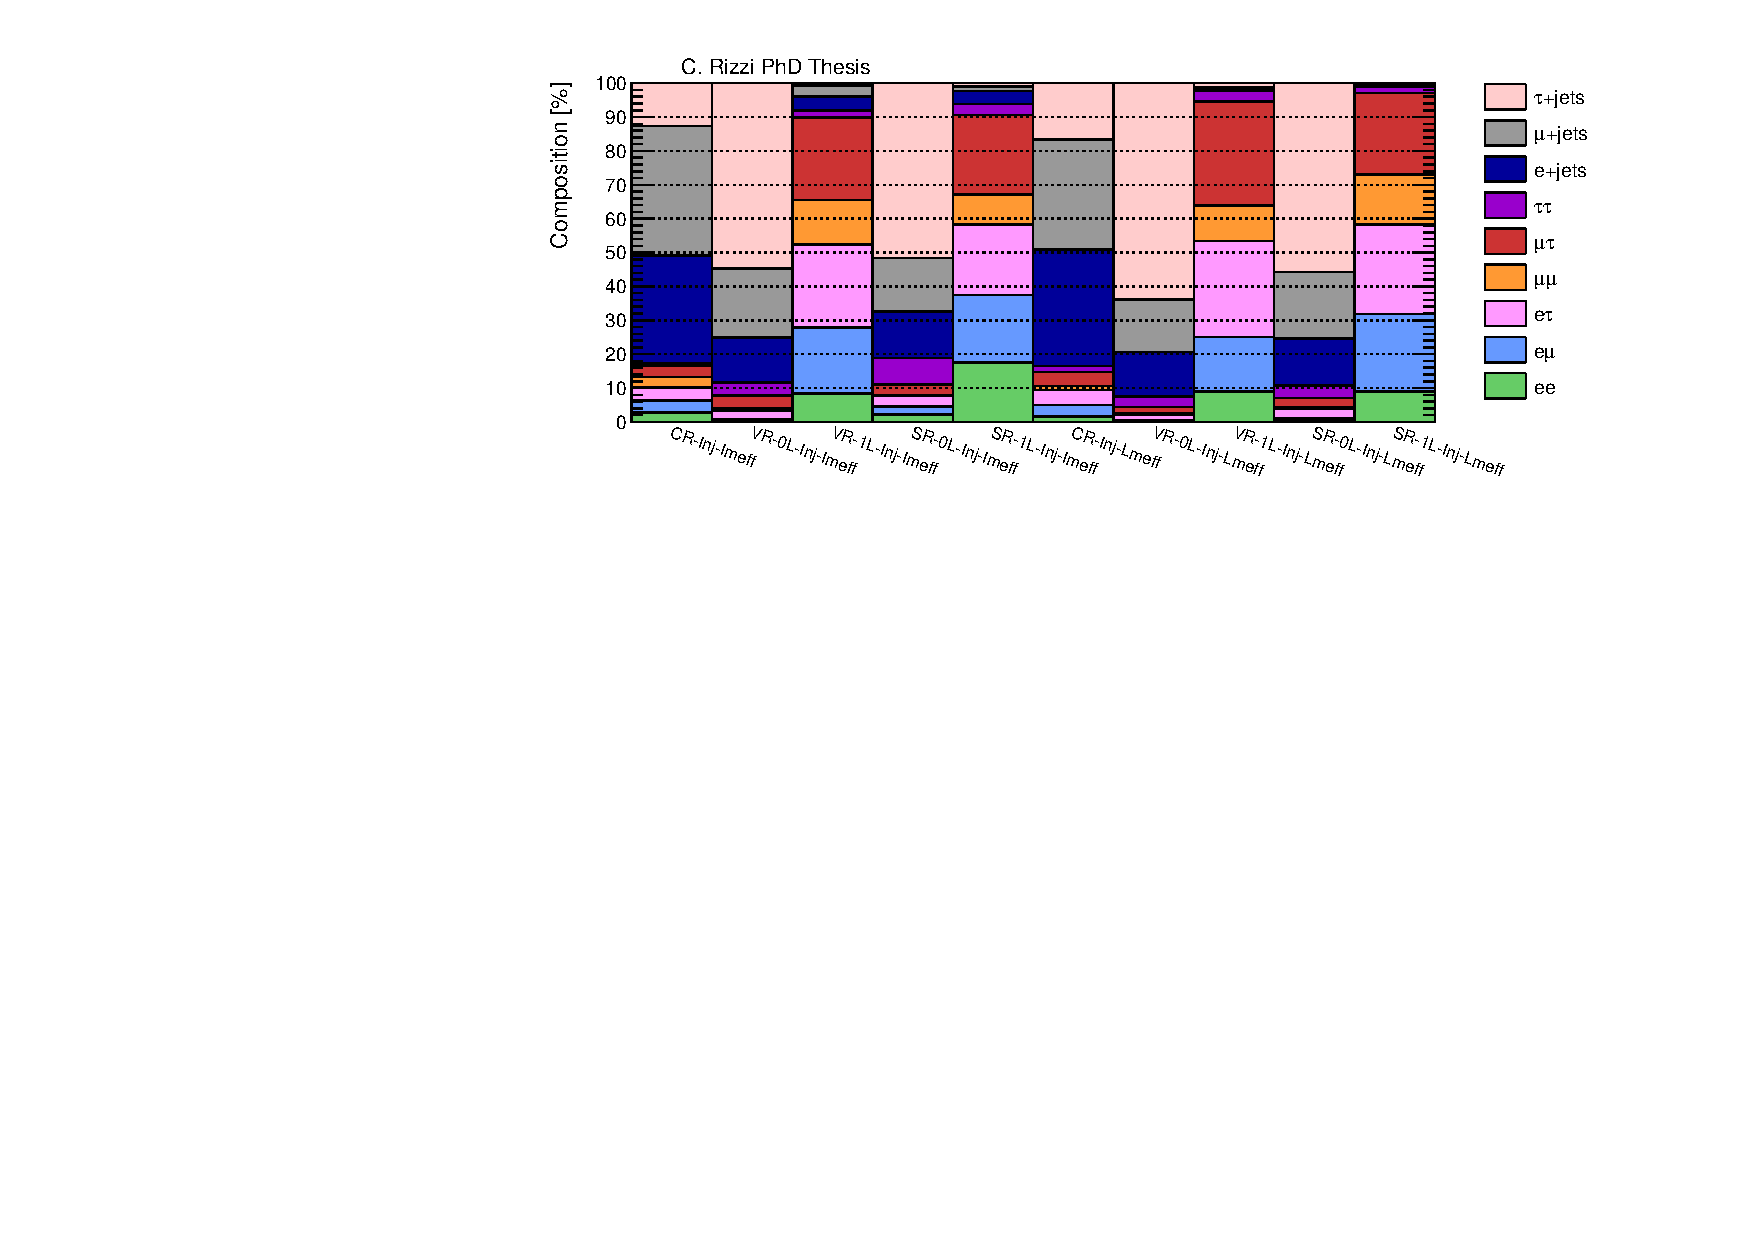
\includegraphics[width=\textwidth]{figures/strong_prod/comp_plots/Inj_tt.pdf}
\caption{Decay mode of the \ttbar background in the the multi-bin regions with intermediate number of jets.}
	\label{fig:ttcomp_Inj}
\end{figure}

\begin{figure}[htbp]
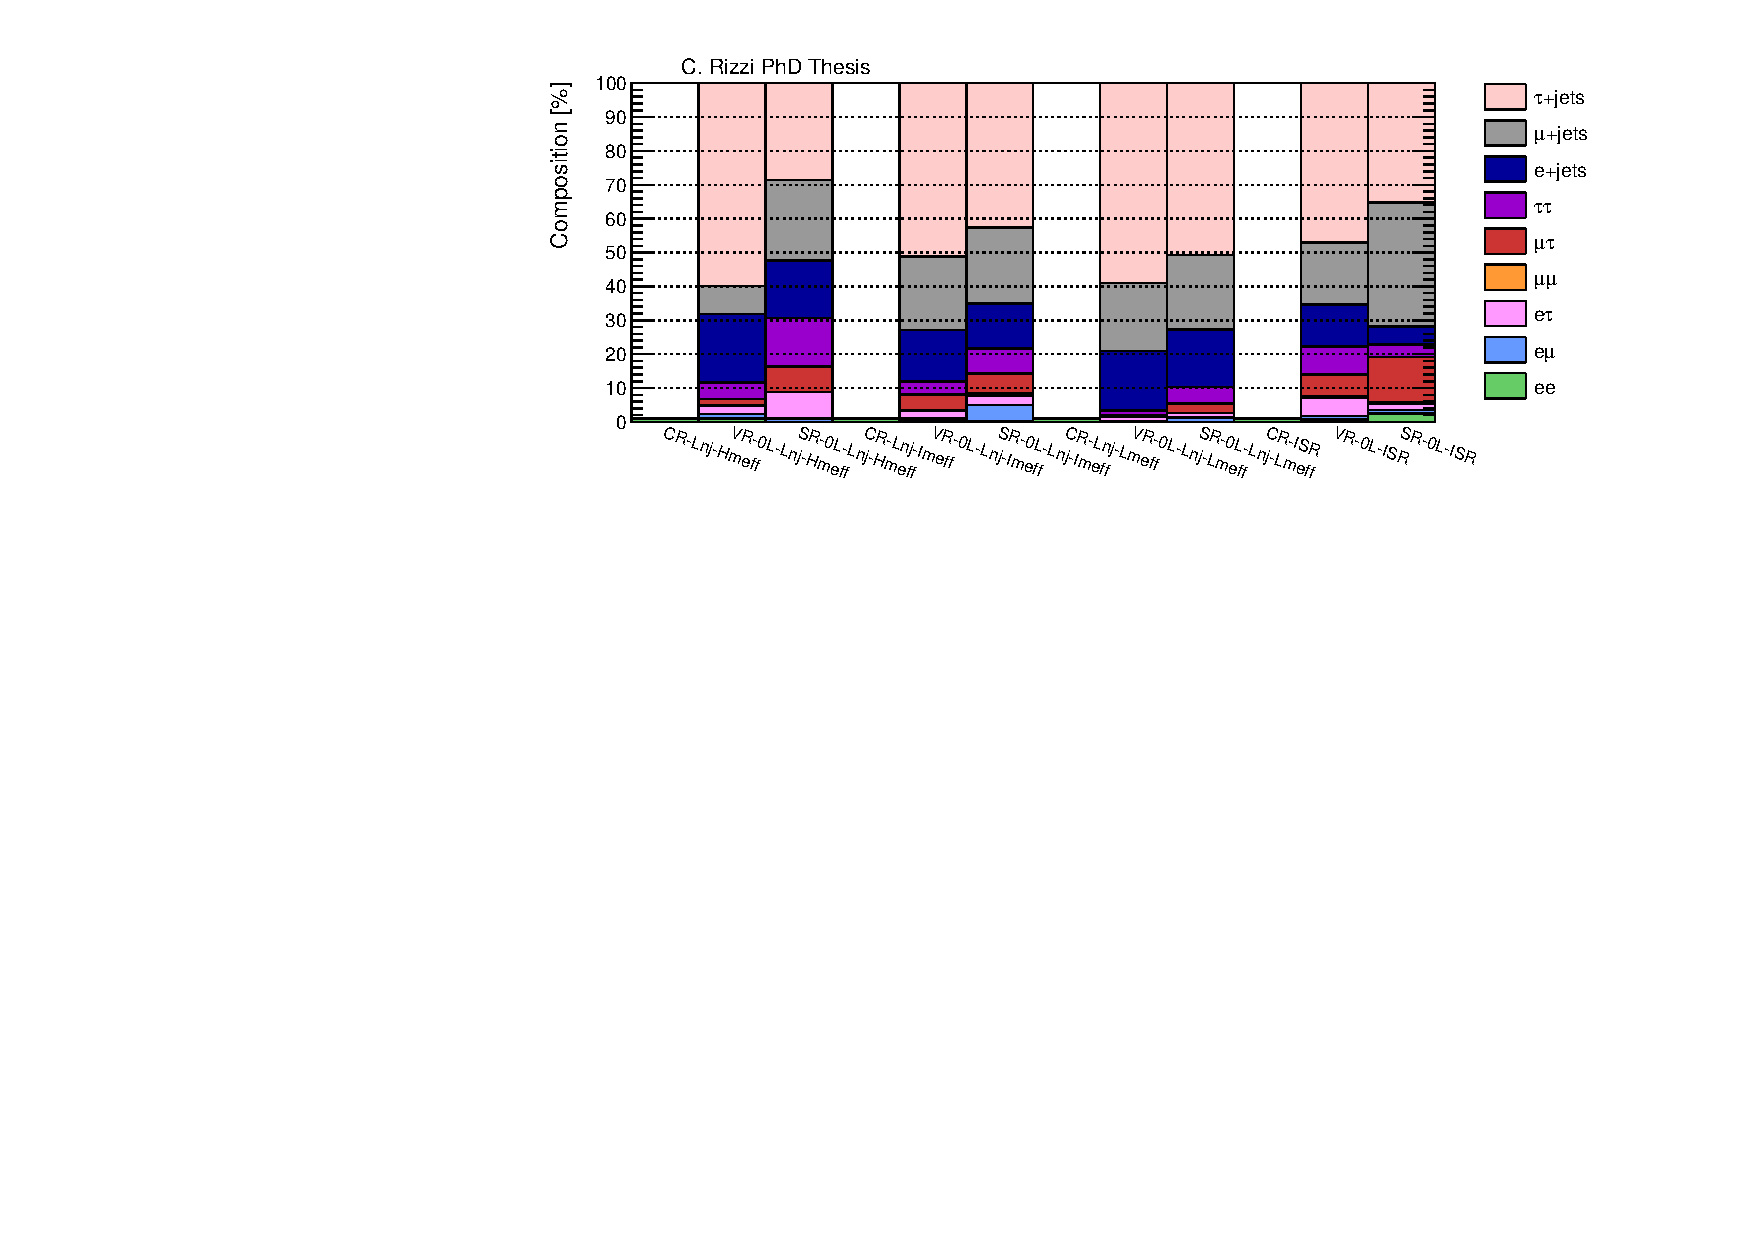
\includegraphics[width=\textwidth]{figures/strong_prod/comp_plots/Lnj_tt.pdf}
\caption{Decay mode of the \ttbar background in the the multi-bin regions with low number of jets.}
	\label{fig:ttcomp_Lnj}
\end{figure}

%%%%


\begin{figure}[htbp]
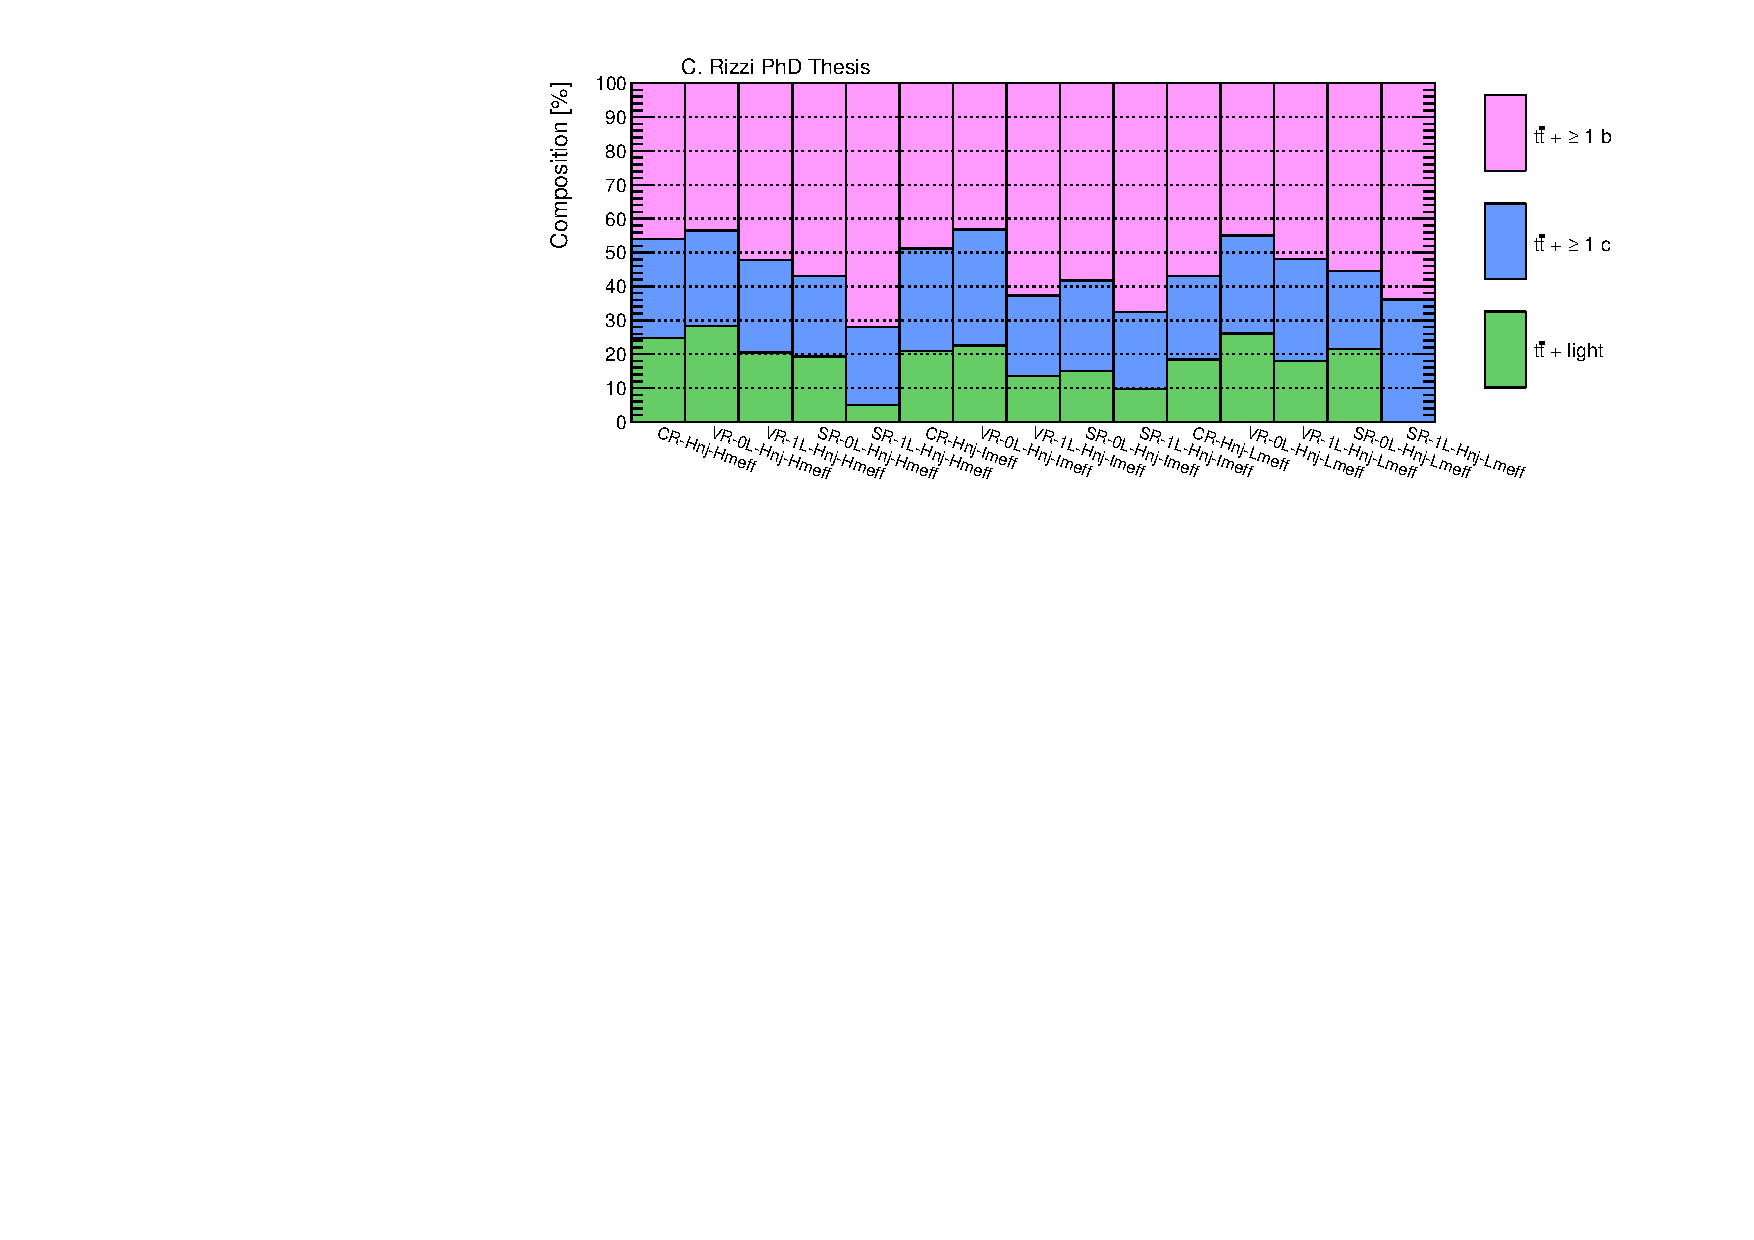
\includegraphics[width=\textwidth]{figures/strong_prod/comp_plots/Hnj_HF.pdf}
\caption{Heavy-flavour composition in the \ttbar background in the multi-bin regions with high number of jets.}
	\label{fig:HFcomp_Hnj}
\end{figure}

\begin{figure}[htbp]
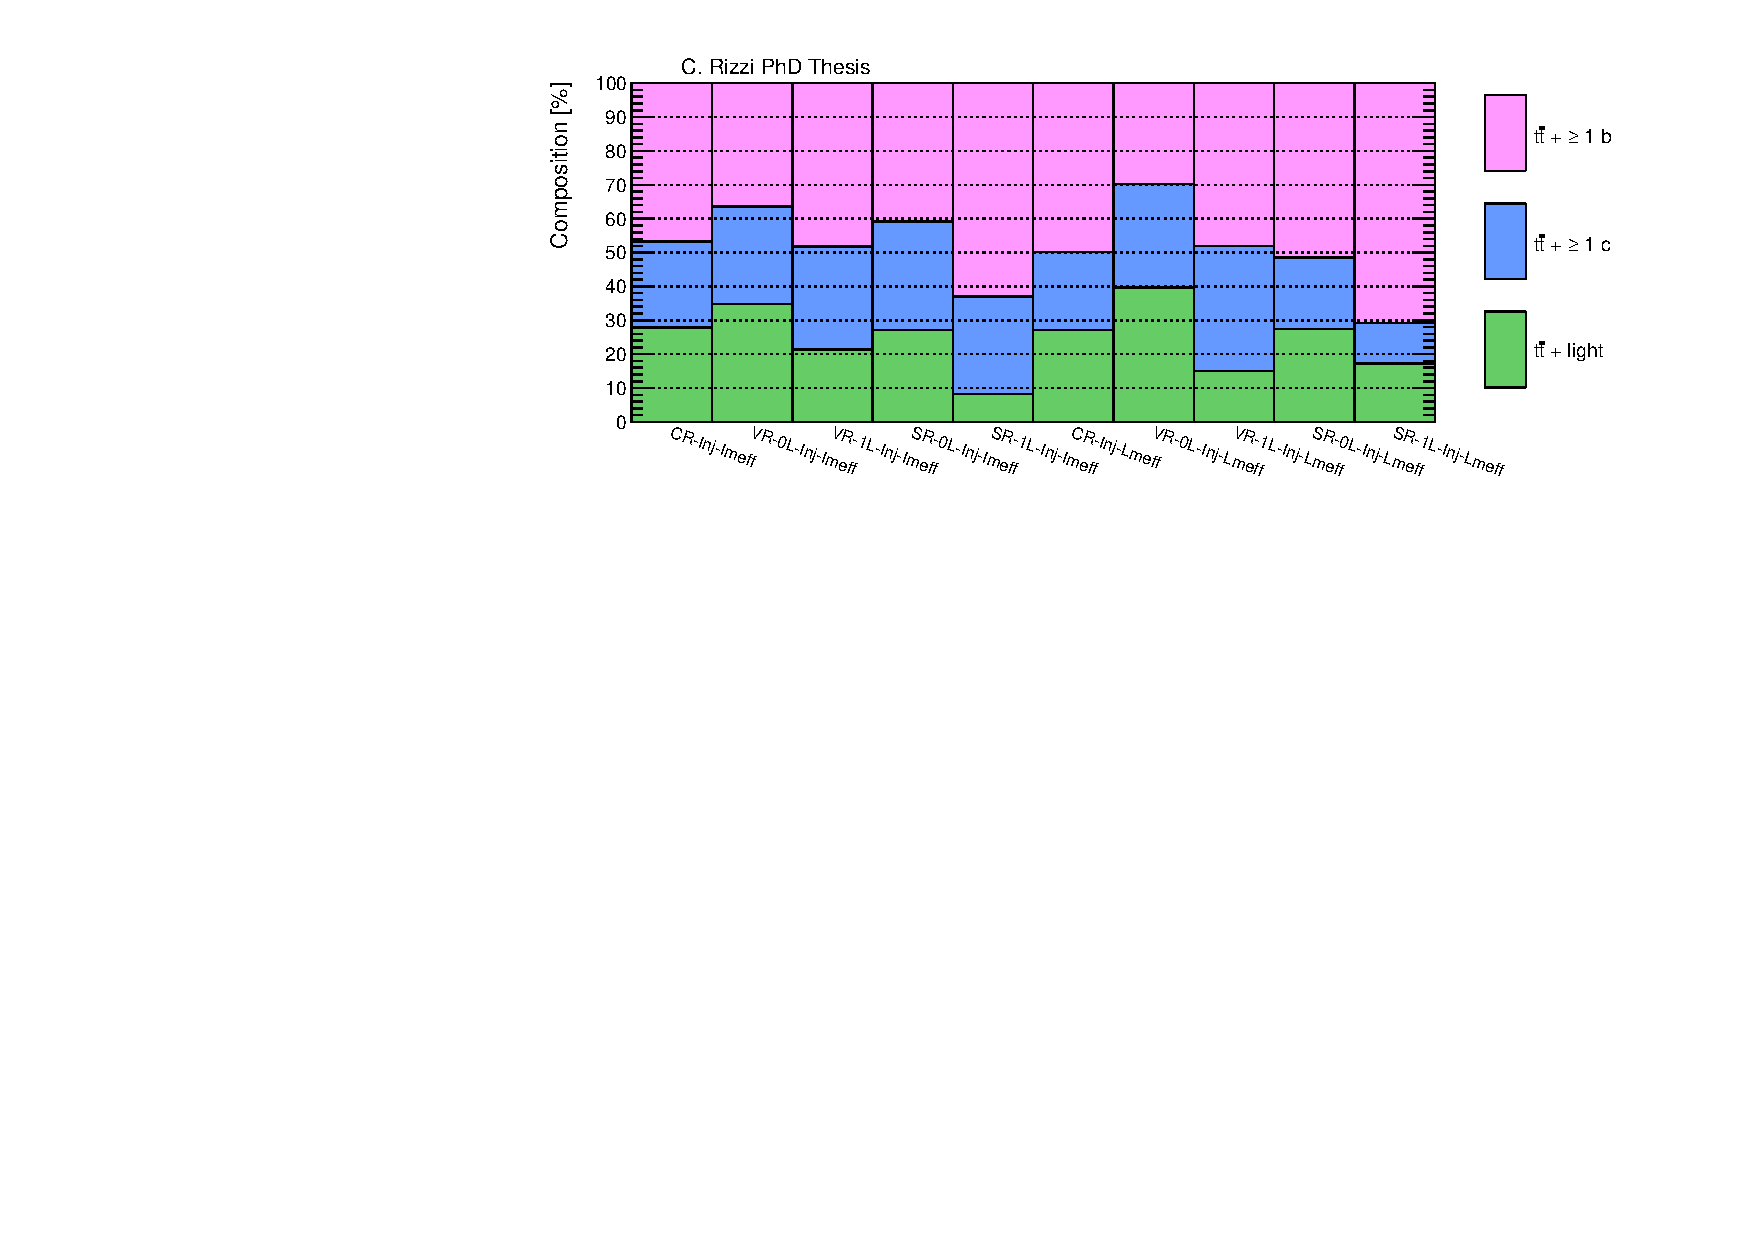
\includegraphics[width=\textwidth]{figures/strong_prod/comp_plots/Inj_HF.pdf}
\caption{Heavy-flavour composition in the \ttbar background in the multi-bin regions with intermediate number of jets.}
	\label{fig:HFcomp_Inj}
\end{figure}

\begin{figure}[htbp]
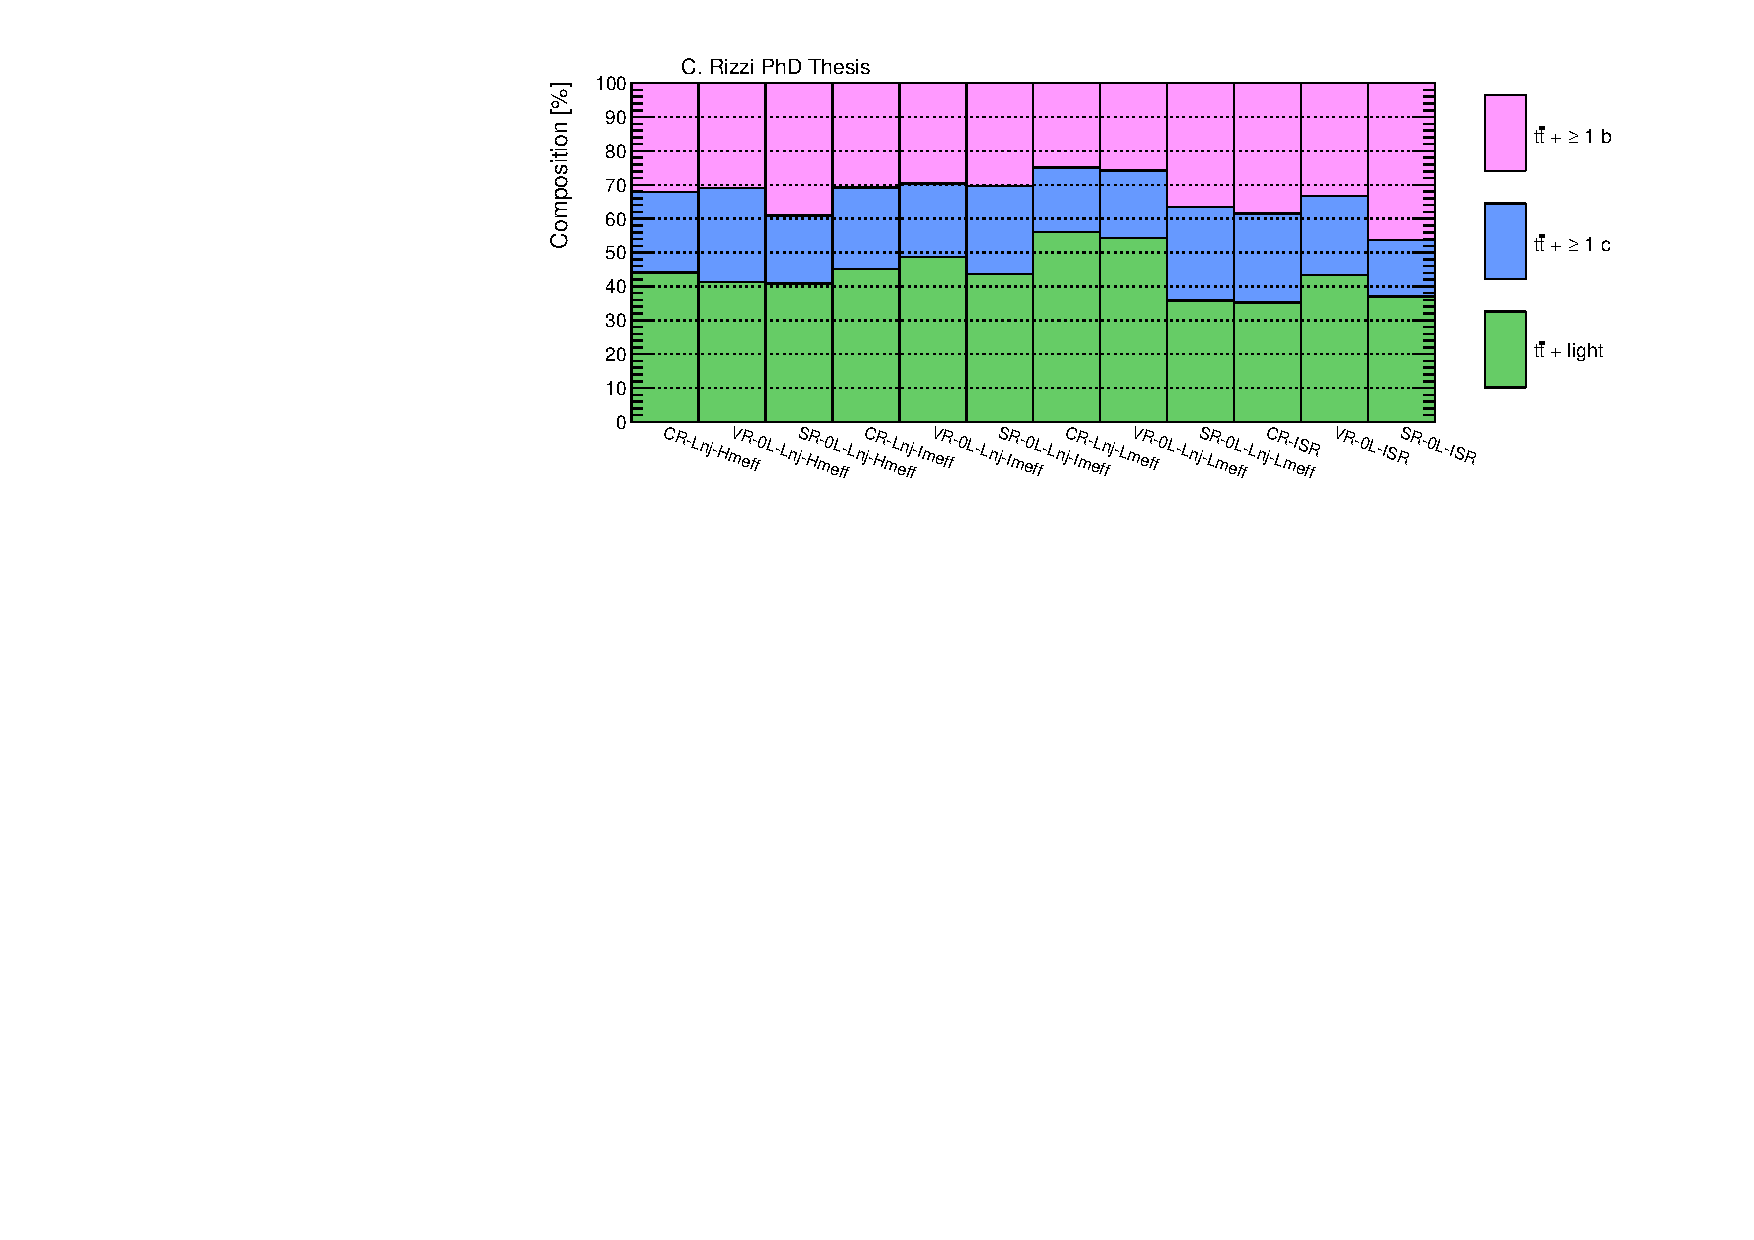
\includegraphics[width=\textwidth]{figures/strong_prod/comp_plots/Lnj_HF.pdf}
\caption{Heavy-flavour composition in the \ttbar background in the multi-bin regions with low number of jets.}
	\label{fig:HFcomp_Lnj}
\end{figure}

\FloatBarrier

\section{Pre-fit data-MC}
\label{sec:strong:dataMC}
In this section we show the pre-fit agreement between data and the \gls{mc} simulation before the fit in the \gls{cr}
in the distribution of the same kinematic variables as in Section \ref{sec:strong:sigbkg}. 
All the plots show in this section do not include systematic uncertainties and include all the relevant \gls{mc} \glspl{sf}. 
In order to investigate a region of the phase space depleted in signal events the requirement on the number
of b-tagged jets is relaxed to $\nbjet \geq 2$. 

\subsection*{Kinematic reweighting}

The modelling of most kinematic variables related to the energy of the event shows a moderate disagreement 
when compared with data in the 1-lepton channel, while in the agreement is good in the 0-lepton channel. 
This is particularly visible in the distribution of \meff, as shown in Figure \ref{fig:strong:datamc:meff_prerw}.

\begin{figure*}[h]
\centering 
\subfigure[]{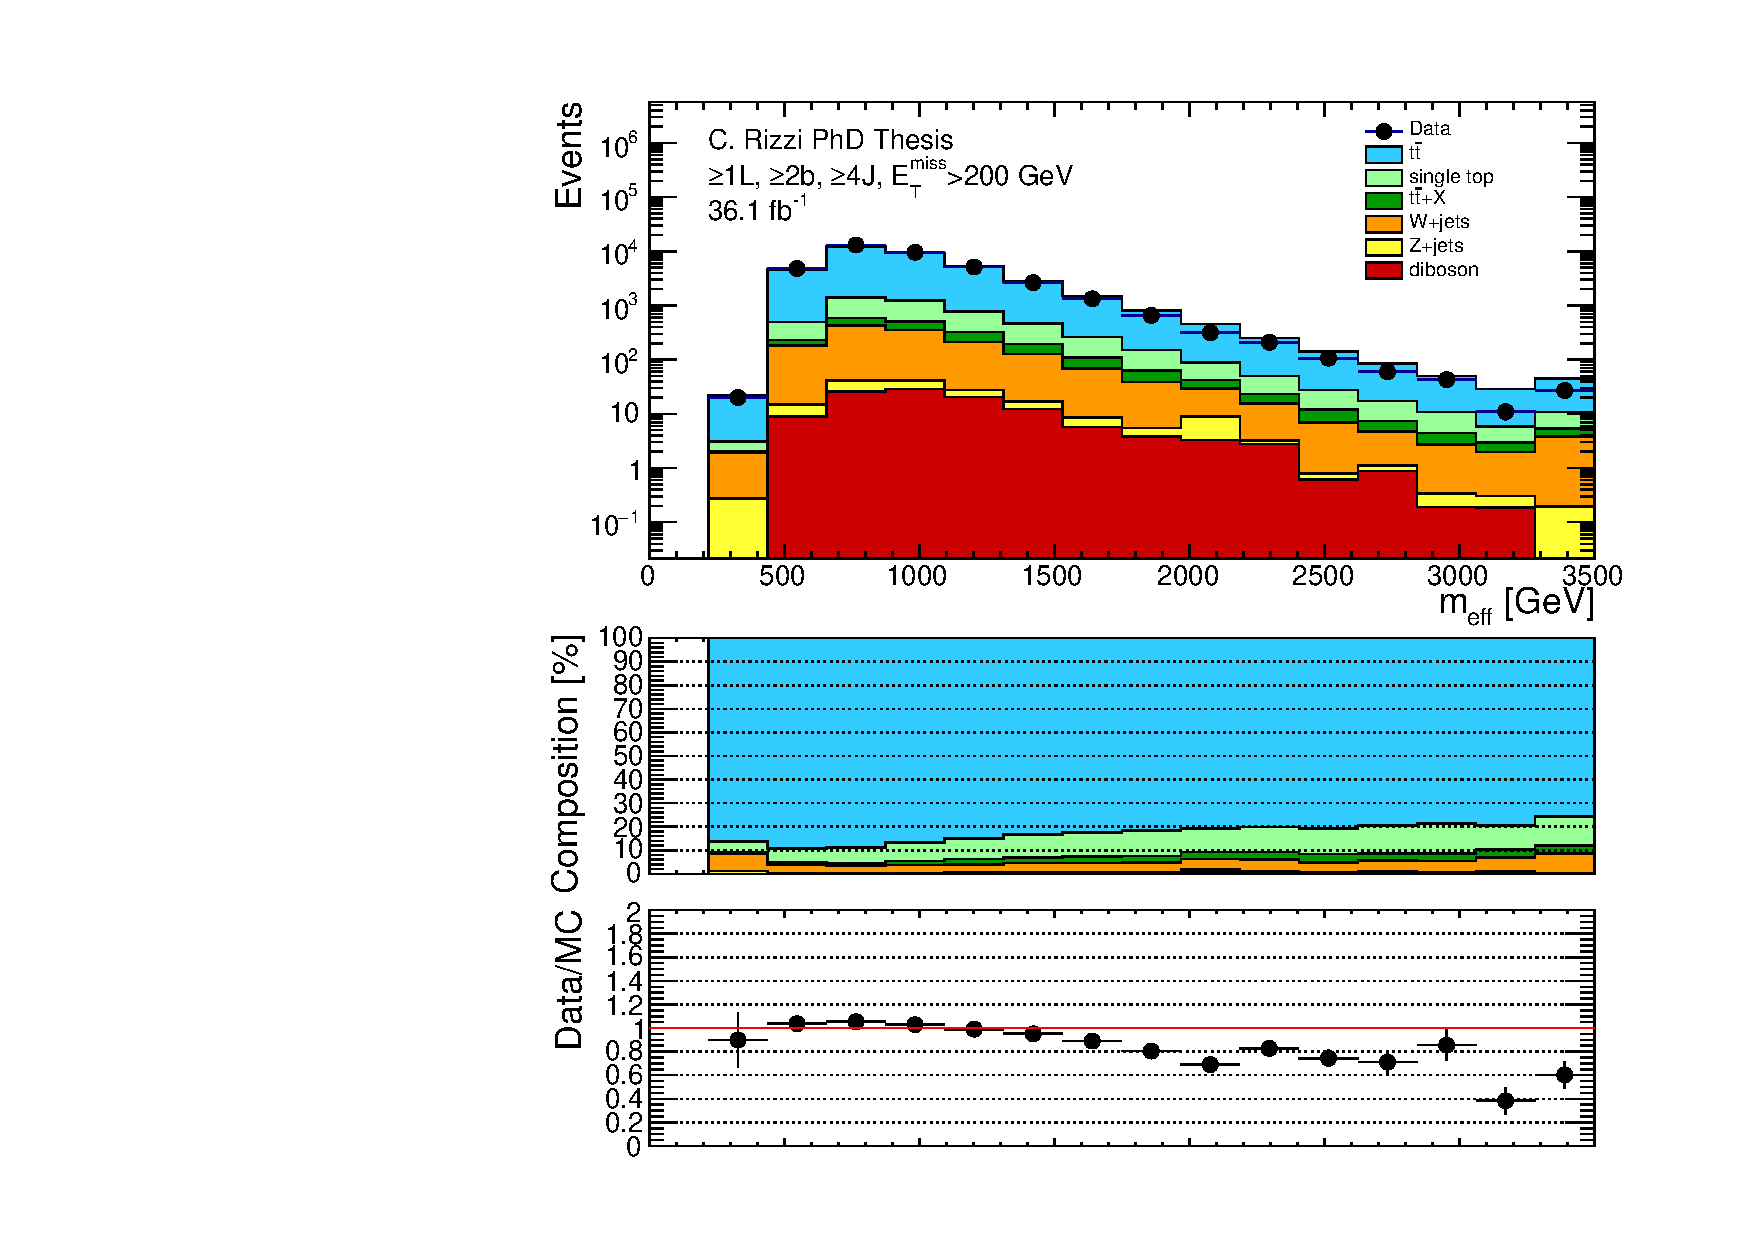
\includegraphics[width=0.49\textwidth]{figures/strong_prod/data_mc/1L_2bin/data_mc_meff_incl.pdf}
\label{fig:strong:datamc:meff_prerw_1L}}
\subfigure[]{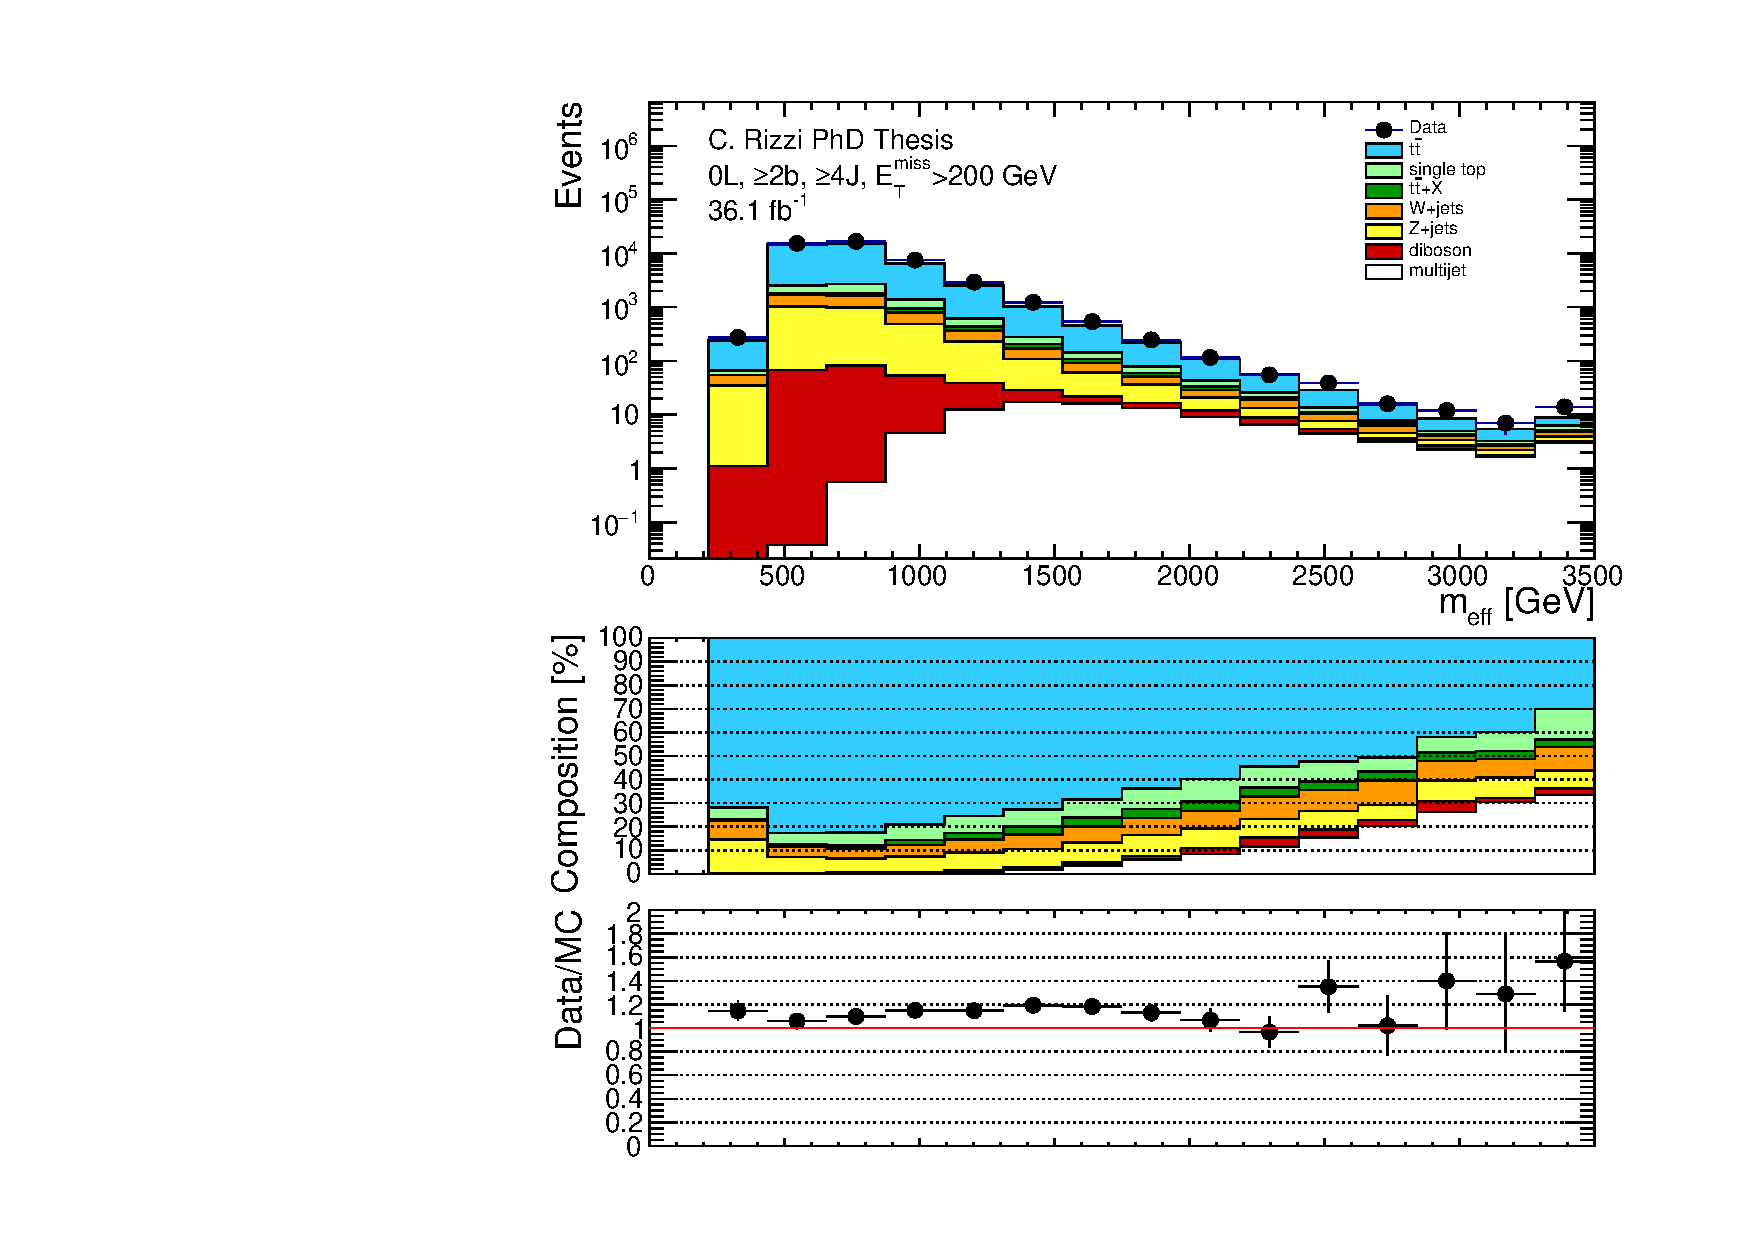
\includegraphics[width=0.49\textwidth]{figures/strong_prod/data_mc/0L_2bin/data_mc_meff_incl.pdf}
\label{fig:strong:datamc:meff_prerw_0L}}
\caption{ \subref{fig:strong:datamc:meff_prerw_1L}
}
\label{fig:strong:datamc:meff_prerw}
\end{figure*}

While the downward trend in the data/MC ratio in the 1-lepton channel is clearly visible in the bottom panel of Figure \ref{fig:strong:datamc:meff_prerw_1L},
Figure \ref{fig:strong:datamc:meff_prerw_0L} shows that this is not present in the 0-lepton channel.
This difference in trends is problematic for the analysis, since all of the \glspl{vr} require at least one signal lepton, 
including the ones used to derive the prediction for 0-lepton \glspl{sr}. 

To mitigate this problem and to have a better estimate of the background in the high-\meff tail, a reweighting is derived 
based on the distribution of \meff in a region that requires exactly two b-jets and low \mtb and is therefore
 orthogonal to all the analysis regions. More details on the reweighting procedure and on its validation are given in Appendix \ref{app:meffrw}.
All the plots in the rest of this section assume that the reweighting has already been applied. 


\subsection*{Data-MC comparison after the reweighting}



\FloatBarrier

\section{Systematic uncertainties}
\label{sec:strong:syst}

The sources of systematic uncertainties discussed in Sections \ref{sec:common_syst} and \ref{sec:common_backgrounds} are included in the analysis.
The relative size of these uncertainties after the fit in the \glspl{cr} is shown in Figures \ref{fig:syst_cutandcount} and \ref{fig:syst_multibin},
for the cut-and-count and multi-bin analyses respectively. 
In the figure, the uncertainties are grouped into:
\begin{itemize}
\item Experimental uncertainties, that contain the sum in quadrature of the detector-related uncertainties 
presented in Section \ref{sec:common_syst}. These are considered for both the background and signal \gls{mc} samples.
The ranking of the different sources of uncertainty changes from region to region; in general the dominant ones are \gls{jes} (that has a 
relative impact on the expected background between 4 and 35\% in the different \glspl{sr}), \gls{jer} (0-26\%) and the uncertainties on the 
b-tagging efficiency and mistagging rate (3-24\%).

\item Theoretical uncertainties, which are the sum in quadrature of the modelling systematics discussed in Section \ref{sec:common_backgrounds}.
In this case the dominant uncertainties are the ones on the modelling of the \ttbar background, whose impact ranges between 5 and 76\%).

\item \gls{mc} statistical uncertainty.

\item Statistical uncertainty in the \glspl{cr}, that is reflected in the uncertainty on the \ttbar scale factor and takes values between 10 and 30\%.

\end{itemize}

The total uncertainty (black line in Figure \ref{fig:syst}) takes into account correlation effects across the different systematic sources, 
and therefore is not the sum in quadrature of the individual components. 

\begin{figure}[htbp]
	\centering
	\subfigure[]{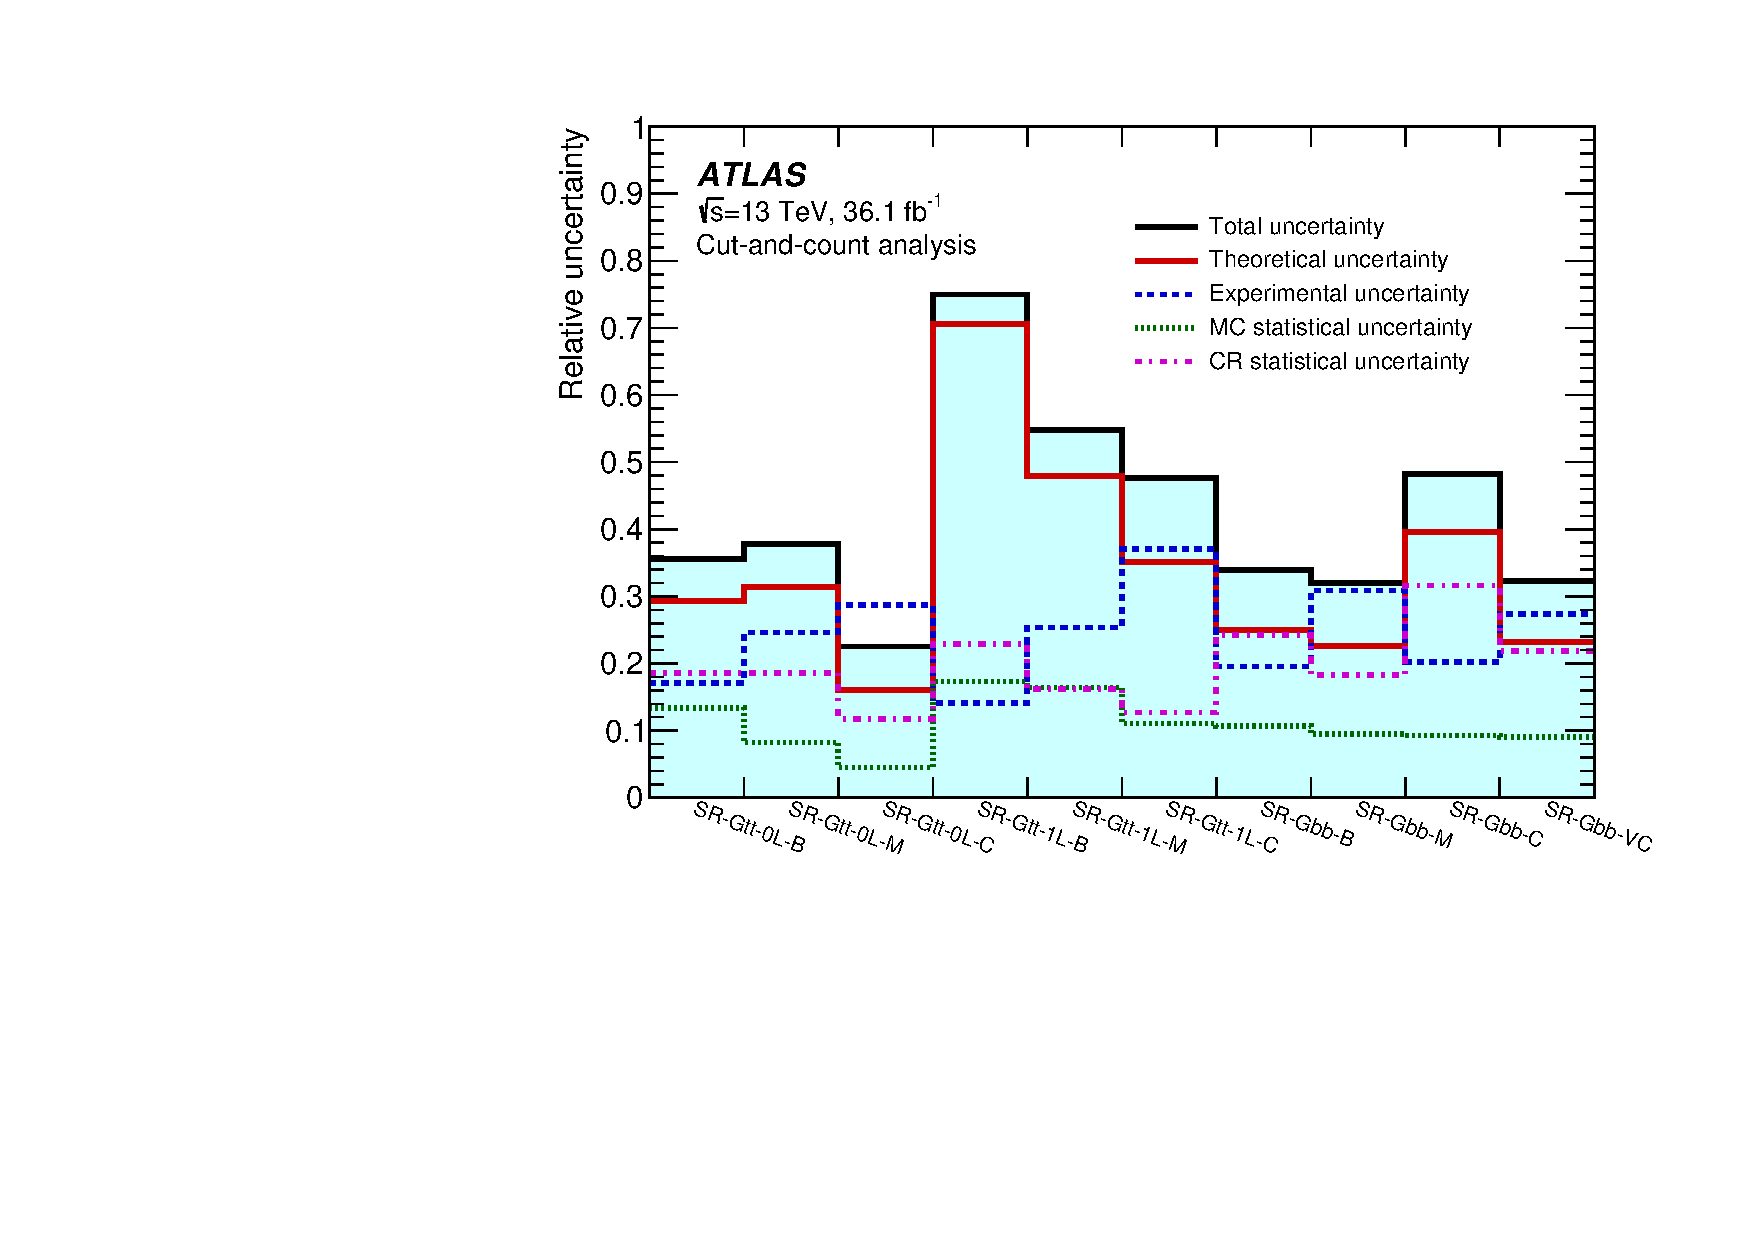
\includegraphics[width=0.85\textwidth]{figures/strong_prod/paper/Cut_and_Count.pdf}\label{fig:syst_cutandcount}}\\
	\subfigure[]{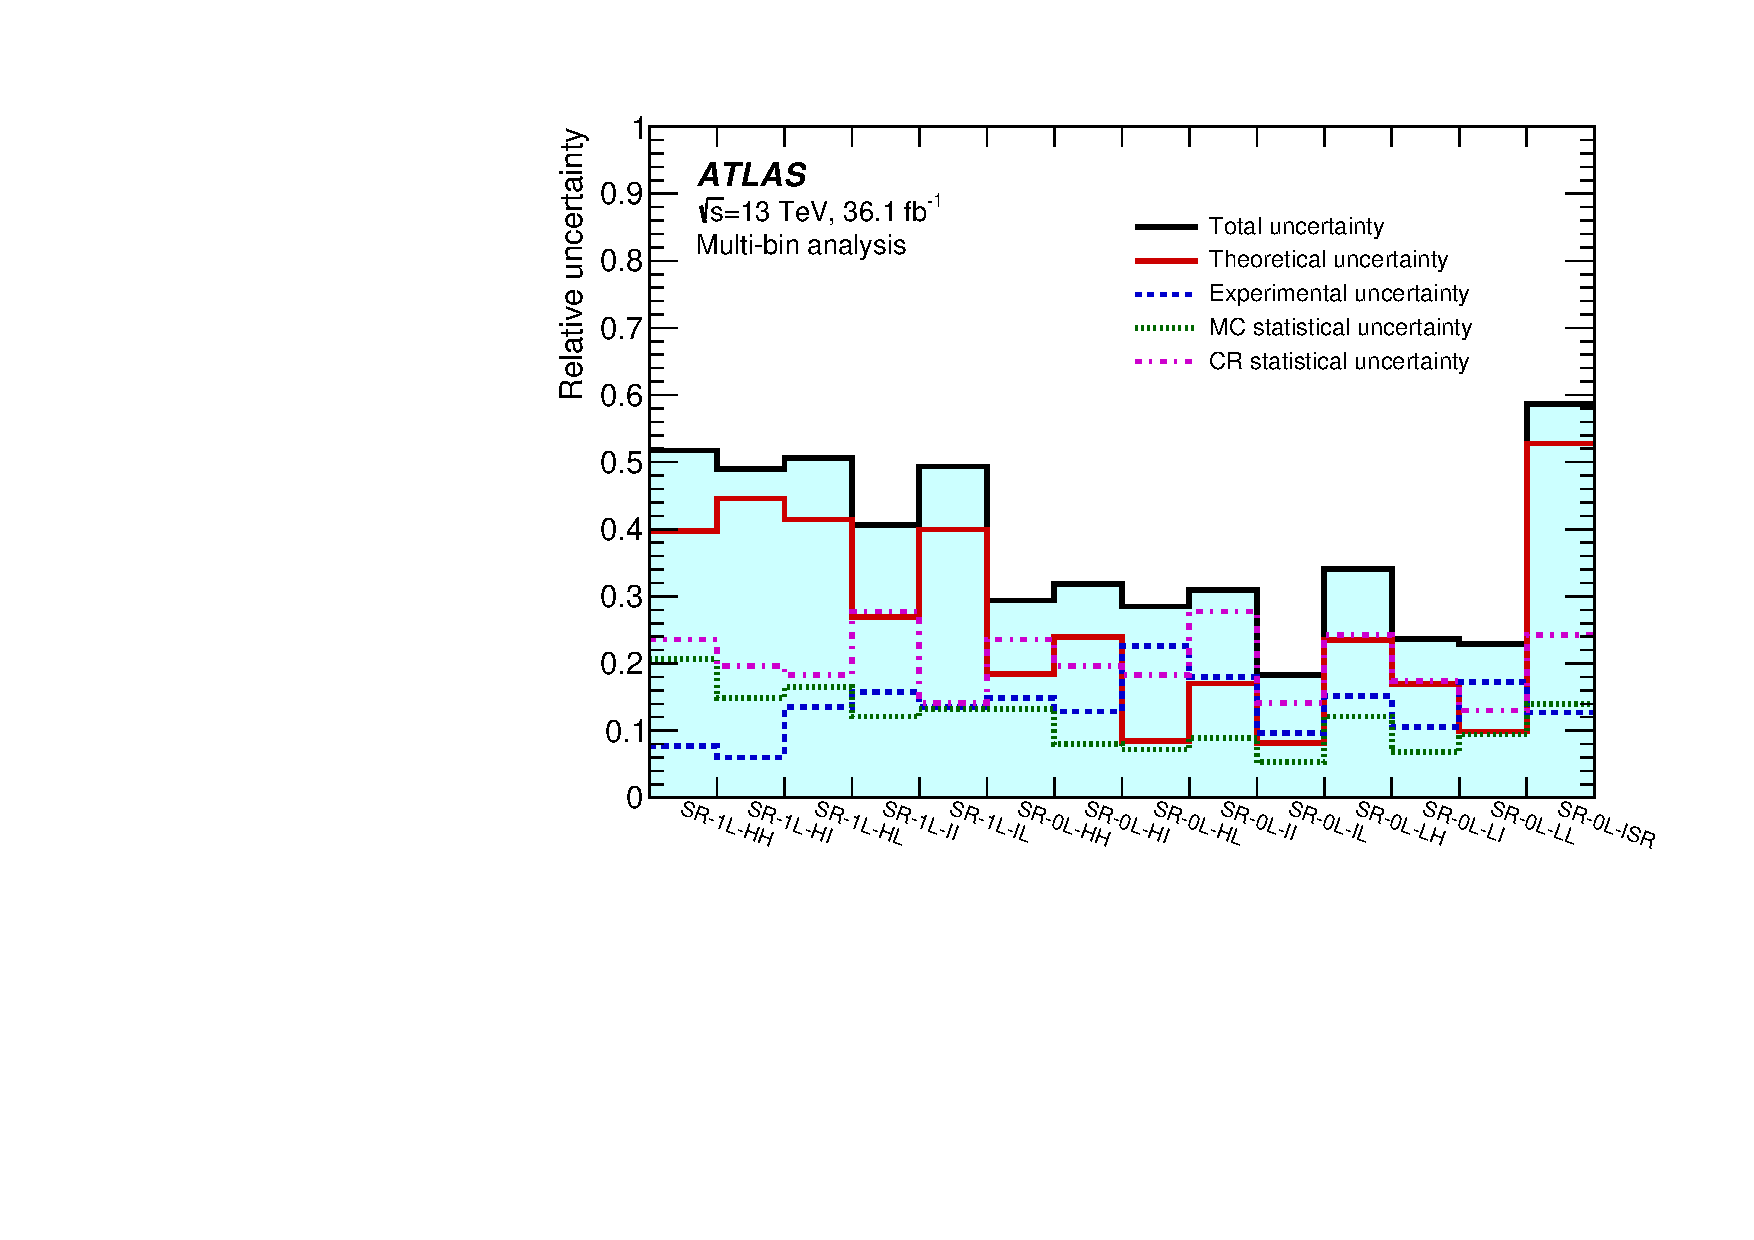
\includegraphics[width=0.85\textwidth]{figures/strong_prod/paper/Multi_bin.pdf}\label{fig:syst_multibin}}\\
	\caption{Relative systematic uncertainty in the background estimate for the \subref{fig:syst_cutandcount} cut-and-count and \subref{fig:syst_multibin} multi-bin analyses. The individual uncertainties can be correlated, such that the total background uncertainty is not necessarily their sum in quadrature.
	} 
	\label{fig:syst}
\end{figure}

\section{Results}
\label{sec:strongprod:results}

The statistical procedures discussed in Chapter \ref{chap:stat} are used to compare the \gls{mc} simulation and the data and extract 
quantitative information on their agreement and on the presence of \gls{bsm} signals. 
The first step is the background-only fit, a maximum-likelihood fit where only the \glspl{cr} are included, as described in Section 
\ref{sec:example_cr}. 
The \ttbar nomralization is a free parameter of the fit, and is therefore adjusted with the number of observed events in the \glspl{cr} 
as constraint.
This procedure accounts for potential mismodellings specific of the phase space close to each \gls{sr}, that are not necessarily 
the same for all the regions in the analysis. Therefore each \gls{cr} is used to derive a normalization factor for the \ttbar background,
independent from the normalization factors derived in the other \glspl{cr}, that is then used to derive the background prediction in the 
corresponding \glspl{sr}. 

The top panel of Figures \ref{fig:pullCR_discovery} and \ref{fig:pullCR_exclusion} shows the pre-fit data-MC agreement in the 
\glspl{cr} of the cut-and-count and multi-bin analyses respectively. In the same figures, the bottom panel 
shows the \ttbar normalization factor derived from the fit in the \glspl{cr} with its uncertainty, driven by the statistical uncertainty 
in the \glspl{cr}.  The systematic uncertainties on the expected number of events are included in the fit as nuisance parameters.
Note that in the case of the cut-and-count analysis the fit is performed separately in each \gls{cr}.
Instead for the multi-bin analysis all the \glspl{cr} are included in the same fit, even though with independent parameters for the 
\ttbar normalization. 
 

\begin{figure}[htbp]
	\centering
	\subfigure[]{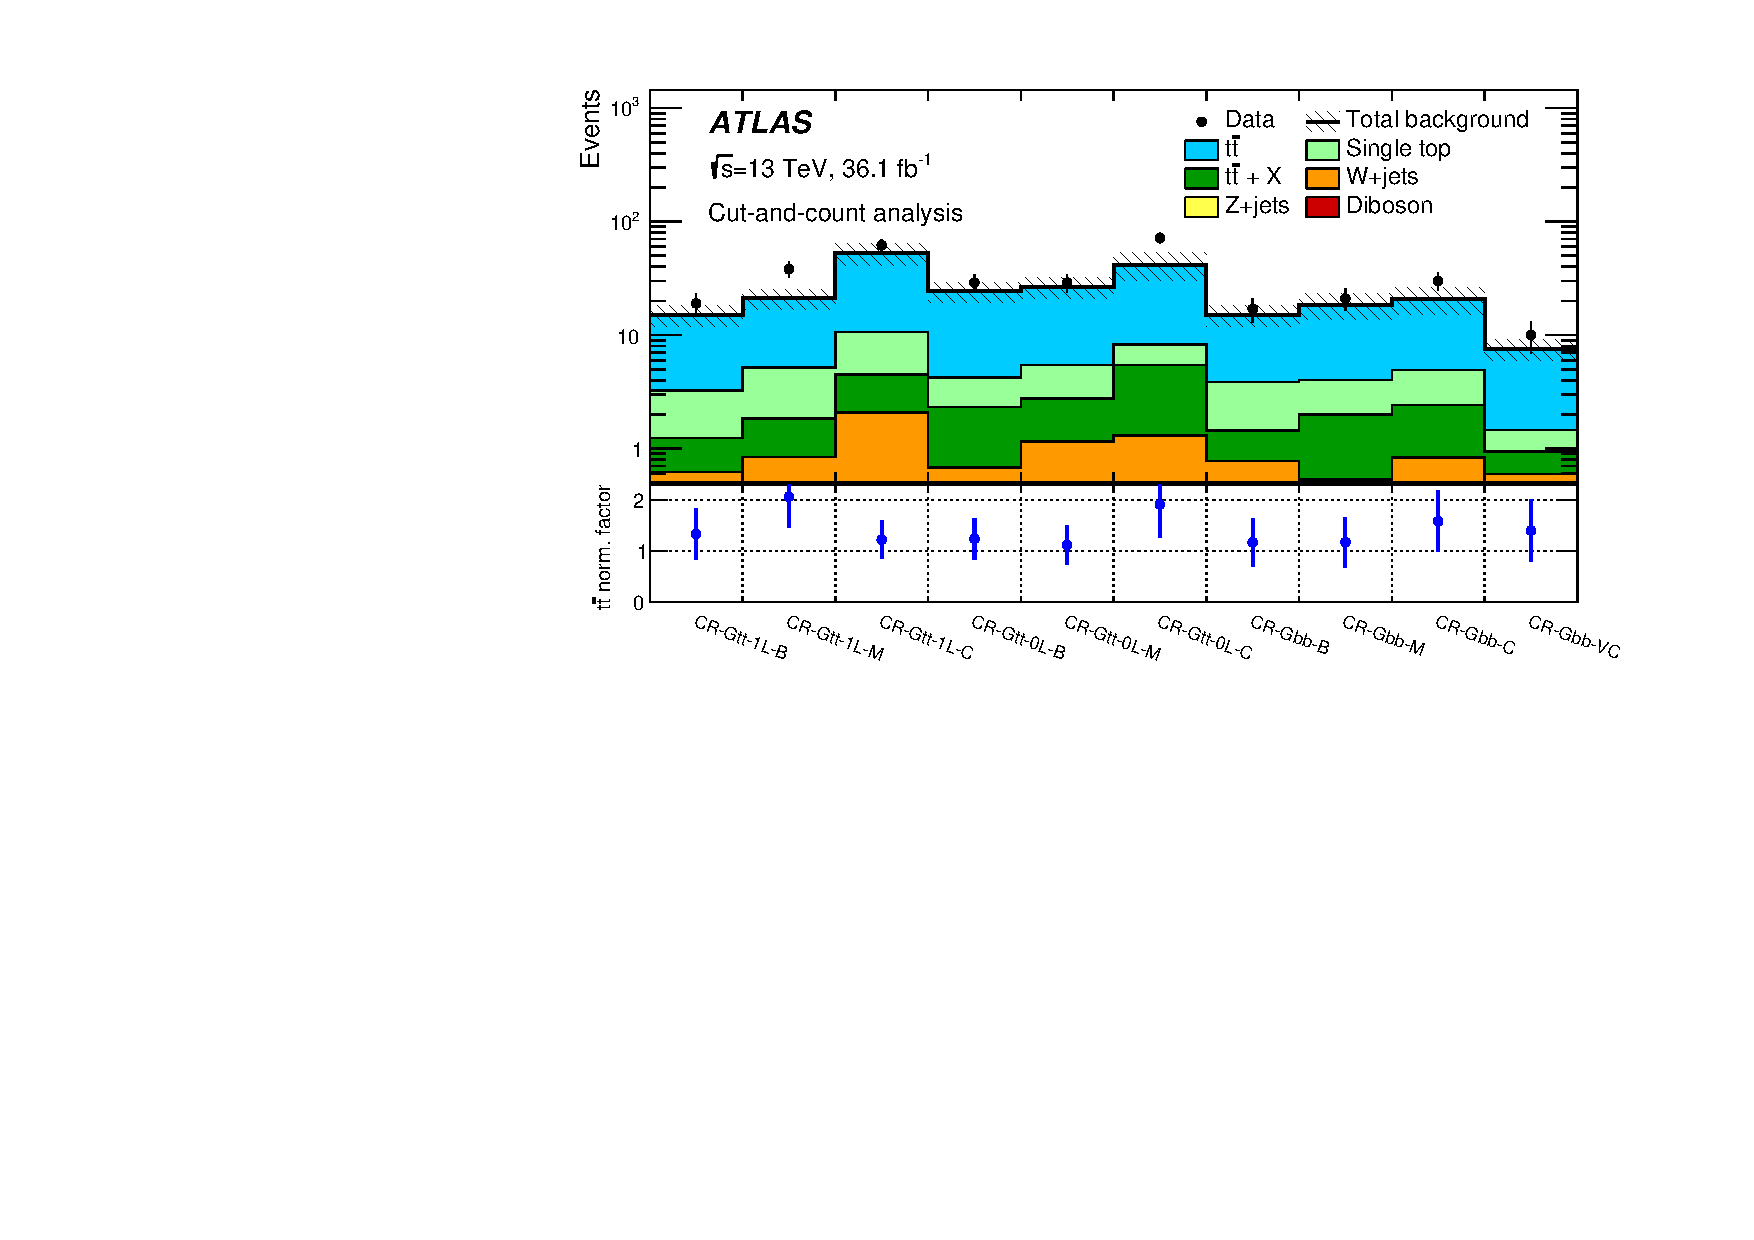
\includegraphics[width=0.9\textwidth]{figures/strong_prod/paper/pulls/histpull_pulls_in_CRs_17_06_23_singlebin.pdf}\label{fig:pullCR_discovery}}
	\subfigure[]{\includegraphics[width=0.9\textwidth]{figures/strong_prod/paper/pulls/histpull_pulls_in_CRs_multichannel_17_06_23.pdf}\label{fig:pullCR_exclusion}}
	\caption{Pre-fit event yield in control regions and related \ttbar
          normalization factors after the background-only fit for
          \subref{fig:pullCR_discovery} 
		the cut-and-count and \subref{fig:pullCR_exclusion} the multi-bin analyses. The upper panel shows 
		the observed number of events and the predicted background yield before the fit.
		The background category \ttbar+X includes \ttbar+W/Z, \ttbar+H and \ttbar\ttbar events. All of these
                regions require at least one signal lepton, for which the
                multijet background is negligible. All uncertainties describes in Section \ref{sec:strong:syst} are included in the uncertainty band.
		The \ttbar normalisation is obtained from the fit
                and is displayed in the bottom panel. 
	} 
	\label{fig:pullCR}
\end{figure}

Figures \ref{fig:pullVR_discovery} and \ref{fig:pullVR_exclusion} show the result of the background-only fit extrapolated to the \glspl{vr} of 
the cut-and-count and multi-bin analysis respectively. The upper panel shows the comparison of the number of predicted and observed events, 
while the bottom panel quantifies the difference between the expected and the observed with the pull, defined as the difference between 
number of observed and expected events divided by the total uncertainty. 

\begin{figure}[htbp]
	\centering
	\subfigure[]{\includegraphics[width=0.9\textwidth]{figures/strong_prod/paper/pulls/histpull_pulls_in_VRs_17_06_23_singlebin.pdf}\label{fig:pullVR_discovery}}\\
	\subfigure[]{\includegraphics[width=0.9\textwidth]{figures/strong_prod/paper/pulls/histpull_pulls_in_VRs_multichannel_17_06_23.pdf}\label{fig:pullVR_exclusion}}\\
	\caption{Results of the background-only fit extrapolated to the VRs of \subref{fig:pullVR_discovery} the cut-and-count and \subref{fig:pullVR_exclusion}
		the multi-bin analyses. The \ttbar normalisation 
		is obtained from the fit to the CRs shown in Figure~\ref{fig:pullCR}. The upper panel shows 
		the observed number of events and the predicted background yield.
		All uncertainties  defined in Section~\ref{sec:syst} are included in the 
		uncertainty band. The background category \ttbar+X includes \ttbar+W/Z, 
		\ttbar+H and \ttbar\ttbar events. The lower panel shows the pulls in 
		each VR. 
	} 
	\label{fig:pullVR}
\end{figure}

The result of the fit extrapolated to the \glspl{sr} and the observed number of events in the \glspl{sr} is finally
shown in Figures \ref{fig:pullSR_discovery} and \ref{fig:pullSR_exclusion} 
for the cut-and-count and the multi-bin analyses respectively. 
No significant excess is observed in the \glspl{sr}; the largest excess is observed in SR-0L-HH, 
one of the regions of the multi-bin analysis, where the pull 2.3 standard deviations. 
The numerical results in the cut-and-count \glspl{sr} are summarized in Table \ref{tab:yield_discovery}.

\begin{figure}[htbp]
	\centering
	\subfigure[]{\includegraphics[width=0.9\textwidth]{figures/strong_prod/paper/pulls/histpull_pulls_in_SRs_17_06_23_singlebin.pdf}\label{fig:pullSR_discovery}}\\
	\subfigure[]{\includegraphics[width=0.9\textwidth]{figures/strong_prod/paper/pulls/histpull_pulls_in_SRs_multichannel_17_06_23.pdf}\label{fig:pullSR_exclusion}}\\
	\caption{Results of the background-only fit extrapolated to the SRs for \subref{fig:pullSR_discovery}
	the cut-and-count and \subref{fig:pullSR_exclusion} the multi-bin analyses. The data in the  SRs are 
	not included in the fit.  The upper panel shows the observed number of events and the predicted background 
	yield. All uncertainties  defined in Section~\ref{sec:syst} are included in the uncertainty band. The background 
	category $\ttbar+X$ includes $\ttbar W/Z$, $\ttbar H$ and $\ttbar \ttbar$ events. The lower panel shows the 
	pulls in each SR.} 
	\label{fig:pullSR}
\end{figure}

\begin{table*}[htbp]
	\centering	
	\renewcommand{\arraystretch}{1.0}
	\begin{tabular}{lccc}
	       \toprule
	       & \multicolumn{3}{c}{SR-Gtt-1L} \\
	       \midrule	
	        Targeted kinematics & B            &   M         &   C               \\[-0.05cm]
	       \midrule
	       Observed events              &  0   &  1 & 2  \\
	       \midrule
	       Fitted background             & 0.5 $\pm$ 0.4 & 0.7 $\pm$ 0.4 & 2.1 $\pm$ 1.0\\
	       \midrule
	       \ttbar\              &  0.4 $\pm$ 0.4 & 0.5 $\pm$ 0.4 & 1.2 $\pm$ 0.8\\
	       Single-top             & 0.04 $\pm$ 0.05 & 0.03 $\pm$ 0.06 & 0.35 $\pm$ 0.28\\
	       $\ttbar+X$          & 0.08 $\pm$ 0.05 & 0.09 $\pm$ 0.06 & 0.50 $\pm$ 0.28\\
	       $Z$+jets            & 0.049 $\pm$ 0.023 & 0.050 $\pm$ 0.023 & $<0.01$ \\
	       $W$+jets              & $<0.01$  & $<0.01$  & 0.024 $\pm$ 0.026\\
	       Diboson             & $<0.01$ & $<0.01$  & $<0.01$ \\
 	       \midrule
	       MC-only background &  0.43 & 0.45 & 1.9 \\
	       \bottomrule
	\end{tabular}

	\vspace{0.4cm}
	
        \begin{tabular}{lccc}
		\toprule
		& \multicolumn{3}{c}{SR-Gtt-0L} \\
		\midrule	
	       Targeted kinematics & B            &   M         &   C               \\[-0.05cm]
	       \midrule
	       Observed events              &  2 & 5 & 28 \\
	       \midrule
	       Fitted background             & 1.5 $\pm$ 0.5 & 3.5 $\pm$ 1.3 & 38 $\pm$ 8\phantom{0} \\
	       \midrule
	       \ttbar\              & 0.9 $\pm$ 0.4 & 1.8 $\pm$ 0.7 & 31 $\pm$ 8\phantom{0} \\
	       Single-top             & 0.21 $\pm$ 0.14 & 0.6 $\pm$ 0.4 & 1.3 $\pm$ 1.1\\   
	       $\ttbar+X$          & 0.12 $\pm$ 0.07 & 0.45 $\pm$ 0.25 & 3.0 $\pm$ 1.6\\
	       $Z$+jets             & 0.06 $\pm$ 0.10 & 0.3 $\pm$ 0.9 & 0.49 $\pm$ 0.31\\
	       $W$+jets            & 0.07 $\pm$ 0.06 & 0.18 $\pm$ 0.15 & 0.67 $\pm$ 0.22\\
	       Diboson             &  0.06 $\pm$ 0.07 & 0.12 $\pm$ 0.07 & $<0.01$\\
 	       Multijet               &  0.09 $\pm$ 0.11 & 0.04 $\pm$ 0.05 & 1.3 $\pm$ 2.1\\
          \midrule
	       MC-only background &   1.3 & 3.3 & 23\\  
	       \bottomrule
	\end{tabular}

	\vspace{0.4cm}
	
	\begin{tabular}{lcccc}
		\toprule
		& \multicolumn{4}{c}{SR-Gbb} \\
		\midrule
          Targeted kinematics & B            	&   	M   		&   C   &   VC                \\[-0.05cm]
		\midrule
		Observed events              & 2 & 2 & 5 & 0\\
		\midrule
		Fitted background           &   2.1 $\pm$ 0.7 & 3.0 $\pm$ 1.0 & 5.8 $\pm$ 1.9 & 4.7 $\pm$ 2.3\\
		\midrule
		\ttbar\            			& 1.2 $\pm$ 0.6 & 1.9 $\pm$ 0.7 & 3.8 $\pm$ 1.3 & 3.1 $\pm$ 1.3\\
		Single-top             		& 0.31 $\pm$ 0.16 & 0.39 $\pm$ 0.16 & 0.46 $\pm$ 0.20 & 0.15 $\pm$ 0.18\\
		$\ttbar+X$             		& 0.12 $\pm$ 0.06 & 0.33 $\pm$ 0.19 & 0.6 $\pm$ 0.4 & 0.19 $\pm$ 0.11\\
		$Z$+jets             		& 0.15 $\pm$ 0.34 & 0.2 $\pm$ 0.6 & 0.6 $\pm$ 1.3 & 0.8 $\pm$ 1.9\\
		$W$+jets             		& 0.12 $\pm$ 0.09 & 0.13 $\pm$ 0.12 & 0.29 $\pm$ 0.19 & 0.37 $\pm$ 0.30\\
		Diboson             		& 0.06 $\pm$ 0.04 & $<0.01$ & $<0.01$ & 0.15 $\pm$ 0.08\\
                Multijet              & 0.10 $\pm$ 0.12 & 0.022 $\pm$ 0.025 & 0.03 $\pm$ 0.04 & 0.016 $\pm$ 0.020\\
		 \midrule
 		MC-only background & 1.9 & 2.7 & 4.4 & 3.9  \\  
		\bottomrule
	\end{tabular}
\caption{Results of the background-only fit extrapolated to the Gtt 1-lepton, Gtt 0-lepton and Gbb SRs in
	the cut-and-count analysis, for the total background prediction and breakdown of the main background sources. 
	The uncertainties shown include all systematic uncertainties. The data in the SRs are not included in the fit. 
	The background category $\ttbar+X$ includes $\ttbar W/Z$, $\ttbar H$ and $\ttbar \ttbar$ events.
	The row ``MC-only background'' provides the total background prediction when the
	$\ttbar$ normalisation is obtained from a theoretical
	calculation~\cite{Czakon:2011xx}. 
	}
	\label{tab:yield_discovery}
\end{table*}


%\clearpage 
\FloatBarrier

\section{Interpretation}
\label{sec:strongprod:limits}

The results described in Section \ref{sec:strongprod:results} are used to set limits on the presence of \gls{bsm} 
signal models. 

\subsection{Model-independent limits}
\label{sec:strong:modelindepUL}

The results of the background-only fit in the cut-and-count \glspl{sr}
are used to place model-independent limits on the number of \gls{bsm} events in the \glspl{sr}. 
This limit is obtained with the \gls{cls} procedure; for each \gls{sr}, a fit similar to the background-only fit is performed 
but the number of observed and expected events (with its uncertainty) is included in the fit as well. 
Any signal contamination in the \glspl{cr} is neglected. 
The limits reported in Table \ref{mod-ind-lim} are obtained with pseudo-experiments, as dissed in Section \ref{sec:stat:example:limits}.

\begin{table}[htbp]
        \centering
        \small
        \begin{tabular*}{0.6\textwidth}{@{\extracolsep{\fill}}lcccc}
                \noalign{\smallskip}\toprule\noalign{\smallskip}
                Signal channel         & $p_0$ (Z)            & $\sigma^{95}_\mathrm{vis}$ [fb]  &  $S_{\textrm obs}^{95}$  & $S_{\textrm exp}^{95}$   \\
                \noalign{\smallskip}\midrule \noalign{\smallskip}
                SR-Gtt-1L-B & $ 0.50~(0.00) $ &  $0.08$ &  $3.0$ & $ { 3.0 }^{ +1.0 }_{ -0.0 }$ \\[1mm]
                SR-Gtt-1L-M & $ 0.34~(0.42)$ &  $0.11$ &  $3.9$ & $ { 3.6 }^{ +1.1 }_{ -0.4 }$ \\[1mm]
                SR-Gtt-1L-C & $ 0.50~(0.00)$ &  $0.13$ &  $4.8$ & $ { 4.7 }^{ +1.8 }_{ -0.9 }$ \\[1mm]
                \noalign{\smallskip}\midrule \noalign{\smallskip}
                SR-Gtt-0L-B & $ 0.32~(0.48)$ & $0.13$ &  $4.8$ & $ { 4.1 }^{ +1.7 }_{ -0.6 }$  \\[1mm]
                SR-Gtt-0L-M & $ 0.25~(0.69)$ &  $0.21$ &  $7.5$ & $ { 6.0 }^{ +2.3 }_{ -1.4 }$ \\[1mm]
                SR-Gtt-0L-C & $ 0.50~(0.00)$ &  $0.39$ &  $14.0$ & $ { 17.8 }^{ +6.6 }_{ -4.5 }$ \\[1mm] %%to be updated
                \noalign{\smallskip}\midrule\noalign{\smallskip}
                SR-Gbb-B & $ 0.50~(0.00) $ &  $0.13$ &  $4.6$ & $ { 4.6 }^{ +1.7 }_{ -1.0 }$  \\[1mm]
                SR-Gbb-M & $ 0.50~(0.00) $ & $0.12$ &  $4.4$ & $ { 5.0 }^{ +1.9 }_{ -1.1 }$ \\[1mm]
                SR-Gbb-C & $ 0.50~(0.00) $ &  $0.18$ &  $6.6$ & $ { 6.9 }^{ +2.7 }_{ -1.8 }$ \\[1mm]
                SR-Gbb-VC & $ 0.50~(0.00) $ &  $0.08$ &  $3.0$ & $ { 4.6 }^{ +2.0 }_{ -1.3 }$\\
                \noalign{\smallskip}\midrule\noalign{\smallskip}
        \end{tabular*}
                \caption{The $p_0$-values and $Z$ (the number of equivalent Gaussian standard deviations), 
        	the 95$\%$ CL upper limits on the visible cross-section
                ($\sigma^{95}_\mathrm{vis}$),
                and the observed and
                expected 95$\%$ CL upper limits on the number of BSM events ($S_{\textrm
                obs}^{95}$ and $S_{\textrm exp}^{95}$). The maximum
              allowed $p_0$-value
              is truncated at 0.5.}
        \label{mod-ind-lim}
\end{table}

\subsection{Model-dependent limits}

The multi-bin analysis is used to place stronger limits on specific signal models. 
The limit setting procedure is repeated for each signal model, this time considering fully the signal contamination in the 
\glspl{cr} and the effect of the modelling and experimental uncertainties on the signal. 
In this case the results are obtained using the the asymptotic approximation \cite{Cowan:2010js} when computing the \gls{cls}.


\begin{figure}[htbp]
	\centering 
	\subfigure[]{\includegraphics[width=0.75\textwidth]{figures/strong_prod/paper/limits/Limits_Gtt.pdf}\label{fig:limits_Gtt}}
	\subfigure[]{\includegraphics[width=0.75\textwidth]{figures/strong_prod/paper/limits/Limits_Gbb.pdf}\label{fig:limits_Gbb}}
	\caption{Exclusion limits in the $\ninoone$ and $\gluino$ mass plane
  		for the \subref{fig:limits_Gtt} Gtt and  \subref{fig:limits_Gbb} Gbb models obtained
		in the context of the multi-bin analysis. The dashed and solid bold lines
		show the 95\% CL expected and observed limits, respectively. The
  		shaded bands around the expected limits show the
                impact of the
  		experimental and background uncertainties. The dotted
  		lines show the impact on the observed limit of the variation of the
  		nominal signal cross-section by $\pm 1 \sigma$ of its theoretical
  		uncertainty. 
		The 95\%~CL expected and observed limits from the ATLAS search based on 2015 data 
  		\cite{Aad:2016eki} are also shown.}
	\label{fig:limits_GbbGtt}
\end{figure}

Figures \ref{fig:limits_Gtt} and \ref{fig:limits_Gbb} show the excluded region of the parameter space for Gtt and Gbb models 
respectively. The dashed blue line shows the expected 95\% \gls{cls} limit, which is the limit we would obtain if the observed number of 
events were identical to the expectation from \gls{sm} only, and the yellow band around it indicates the effect of the 
uncertainty on the background prediction. The observed limit is shown with a solid red line, and the dotted red lines show the impact 
of the signal systematic uncertainties on the signal modelling (discussed in Section \ref{sec:strong:signalxsec}). 
Both in the case of the Gtt and Gbb models, the observed limit is weaker that the expected. 
This particularly evident for Gtt models with massless neutralino, where the limit is driven by SR-0L-HH, which has the larges deviation 
between expected and observed number of events.
The observed exclusion limit for massless neutralino is at around 1.97 and 1.92 for the Gtt and Gbb models respectively;
the sensitivity improves by 300 GeV and 450 GeV with respect to the Gbb and Gtt sensitivity obtained from the analysis of the 
2015 data \cite{Aad:2016eki}, shown with dashed black lines in Figure \ref{fig:limits_GbbGtt}. 
Note that the improvement in observed limits 
(comparing the solid black and the solid red lines) is much lower than that, since the analysis in Ref. \cite{Aad:2016eki}
observed a slight deficit while this analysis observes a slight excess. 

As discussed in Section \ref{sec:strong:signalmodel}, the results of the multi-bin analysis are also used to place 
limits on a more realistic model, where the \gls{br} of the gluino can decay to $ t \bar{t} \ninoone$, $ b \bar{b} \ninoone$, 
or $t \bar{b} \chinoonem$ (where the $\chinoonem$ then decays to $\ninoone$ and soft fermions). All combinations of different \gls{br}
to these three decay modes with a unitary constraint on their sum are considered. 
The inclusion of the gluino \glspl{br} as additional parameters makes it impossible to show the results in the two-dimensional plane
defined by the masses of the gluino and the neutralino (as it was the case for the simpler Gtt and Gbb models).
Instead, the limits are presented in the $B(\gluino \to t \bar{t} \ninoone)$ vs. $B(\gluino \to b \bar{b} \ninoone)$ plane 
(assuming that $B(\gluino \to t \bar{b} \chinoonem) = 1 - B(\gluino \to t \bar{t} \ninoone) - B(\gluino \to b \bar{b} \ninoone)$), 
and only a few selected mass points are considered.  

Figure \ref{fig:limit_br_fixed_neu} shows the 95\% \gls{cls} exclusion limit for signal models with $m_{\ninoone} = 1$ GeV and 
$m_{\gluino} = 1.8$, 1.9 and 2.0 TeV. The solid and dashed lines show respectively the observed and expected limits for the different 
mass hypothesis, distinguished by the different colors. The hashing indicates which side of the plane is excluded. 
Due to the mild excesses observed in the multi-bin analysis, the observed limits are weaker than the expected. 
In particular, for a gluino mass of 1.8 TeV, we expect to exclude the entire \gls{br} plane, while the "pure Gtb" corner 
in the bottom left (where both $B(\gluino \to t \bar{t} \ninoone)$ and $B(\gluino \to b \bar{b} \ninoone)$ are close to zero) 
is not excluded, and none of the points are excluded for a gluino mass of 2.0 TeV. 

Figure \ref{fig:limit_br_fixed_glu} shows instead three signal mass hypothesis with a gluino mass of 1.9 TeV 
and $m_{\ninoone} = 1$, 600 and 100 GeV. Also in this case the observed limits are less stringent than the expected, leaving 
not-excluded areas also for signals that we expect to exclude for any \gls{br}, such as the one with neutralino mass of 600 GeV.
ma

\begin{figure}[htbp]
	\centering
	\subfigure[]{\includegraphics[width=0.63\textwidth]{figures/strong_prod/paper/limits/triangle_UL_massless_neutralino.pdf}\label{fig:limit_br_fixed_neu}}
	\subfigure[]{\includegraphics[width=0.63\textwidth]{figures/strong_prod/paper/limits/triangle_UL_1900_gluino.pdf}\label{fig:limit_br_fixed_glu}}
	\caption{Exclusion limits in the $\gluino \to t \bar{t} \ninoone$ and $\gluino \to b \bar{b} \ninoone$
		branching ratio plane assuming \subref{fig:limit_br_fixed_neu} a neutralino mass of 1 GeV and various gluino masses 
		(1.8, 1.9 and 2.0 TeV) and \subref{fig:limit_br_fixed_glu} a gluino mass of 1.9 TeV and three neutralino masses (1, 600 and 1000 GeV). 
		In \subref{fig:limit_br_fixed_neu}, the expected limit for a gluino mass of 1.8 TeV follows the plot axes, meaning that the whole plane is 
		expected to be excluded at 95\% CL.
		The dashed and solid bold lines show the 95\% CL expected and observed limits, respectively. The hashing indicates which side of the line 
		is excluded. The upper right half of the plane is forbidden by the requirement that the sum of branching ratios does not exceed 100\%.}
\end{figure}

\FloatBarrier

\section{Comparison of cut-and-count and multi-bin strategies}

In this analysis, the results of the multi-bin analysis are used to set model-dependent limits on selected signal models.
Also the regions cut-and-count analysis, used to set the model-independent limits in Section \ref{sec:strong:modelindepUL}, 
can be used to provide a statement on specific signal models. The different regions of the cut-and-count analysis are not orthogonal 
and therefore can not be combined in a single statistical fit, but they can still be "visually combined" in a single exclusion contour 
by selection for each mass point the cut-and-count region with the best expected sensitivity, and this contour can be compared 
with the contour obtained with the multi-bin approach.
This is shown in Figures \ref{fig:limits_Gtt_comp} and \ref{fig:limits_Gbb_comp} for the Gtt and Gbb models respectively.
Since we want to make a statement on the sensitivity of the two strategies, we compare only the expected exclusion contours 
(in blue for the cut-and-count analysis, in pink for the multi-bin analysis) and not the observed exclusion. 
The grey numbers on the figures represent the relative difference in expected upper limit on the signal strength: 
a negative number indicates a stronger limit from the multi-bin analysis. 
In the case of the Gtt grid in Figure \ref{fig:limits_Gtt_comp}, the multi-bin approach provides an improvement in 
expected upper limit of $\approx$30\% in the bulk of the mass plane, and up to $\approx$50\% for the more challenging 
kinematic regime where the mass of the neutralino is closer to the mass of the gluino.
In terms of exclusion contour, this translates in an expected limit about 70 GeV stronger for massless neutralino.
In the case of the Gbb signal models, while it is still true that for most of the mass points the expected limit on the 
signal strength is better with the multi-bin approach, for the region of the parameter space with intermediate gluino and 
neutralino masses the cut-and-count analysis provides a stronger sensitivity.
This is balanced by a better sensitivity of the multi-bin strategy for $m_{\gluino} \approx 2$ TeV, $m_{\ninoone} \approx 700$
GeV (where the cut-and-count approach shows the drawback of a switch in best-expected region for neighboring mass points),
and the two strategies have the same limit for massless neutralino. 
The reason of the different relative performance of multi-bin and cut-and-count approaches in the Gtt and Gbb signal 
models relies on the optimization strategy of the multi-bin analysis, that favors Gtt: the regions with intermediate 
number of jets, that could still be sensitive to Gbb models, are optimized based on Gtt signal benchmarks.



\begin{figure}[htbp]
	\centering 
	\subfigure[]{\includegraphics[width=0.75\textwidth]{figures/strong_prod/extra/UL_comp_combi_multich_Gtt.pdf}\label{fig:limits_Gtt_comp}}
	\subfigure[]{\includegraphics[width=0.75\textwidth]{figures/strong_prod/extra/UL_comp_combi_multich_Gbb.pdf}\label{fig:limits_Gbb_comp}}
	\caption{Exclusion limits in the $\ninoone$ and $\gluino$ mass plane
  		for the \subref{fig:limits_Gtt_comp} Gtt and  \subref{fig:limits_Gbb_comp} Gbb models obtained
		in the context of the multi-bin analysis (pink line) and of the cut-and-count analysis (blue line). 
		The gray numbers show the relative difference in expected \gls{ul} between the multi-bin and the cut-and-count analysis: a negative number shows a lower expected \gls{ul} for the multi-bin analysis.}
	\label{fig:limits_GbbGtt_comp}
\end{figure}

%\section{Results in the context of the ATLAS SUSY group}


\FloatBarrier
\section{Update with 2017 data-taking periods}
\label{sec:strong:r21}

The mild excess observed in the multi-bin region SR-0L-HH motivated checking the results with the 2017 data-taking periods 
as soon as they have become available. 
The analysis has been reproduced with all the data collected by the \gls{atlas} experiment in 2015, 2016 and 2017, 
for a total integrated luminosity of 79.8 \ifb. 
Both the cut-and-count and multi-bin regions have been updated in Ref. \cite{ATLAS-CONF-2018-041}, 
but in this section we present only the results 
of the multi-bin regions, since the main purpose is the follow up of the excess in the analysis of the 2015-2016 data.
Differences in the object definition that occurred due to a change in the \gls{atlas} software release between the 
two analyses are not discussed in this section and do not impact sensibly the physics results, more details can be found 
in Ref. \cite{ATLAS-CONF-2018-041}.


\subsection{Results}

The results of the fit in the \glspl{cr} extrapolated to the \glspl{vr} and \glspl{sr} are shown in Figures 
\ref{fig:pullVR_R21} and \ref{fig:pullSR_R21} respectively. 
We can see that there is good agreement with the predicted background in the \glspl{vr}, and the \glspl{vr} do now show any 
significant deviation from the expectations. 
In particular, the excess in SR-0L-HH is no longer present. 

%\begin{figure}[htbp]
%	\centering
%	\subfigure[]{\includegraphics[width=0.9\textwidth]{figures/strong_prod/R21/multibin/histpull_grouping_VR.pdf}\label{fig:pullVR_R21}}\\
%	\subfigure[]{\includegraphics[width=0.9\textwidth]{figures/strong_prod/R21/multibin/histpull_grouping_SR.pdf}\label{fig:pullSR_R21}}\\
%	\caption{Results of the background-only fit extrapolated to the \glspl{vr} for \subref{fig:pullVR_R21}
%	 and to the \glspl{sr} \subref{fig:pullSR_R21} of the multi-bin analyses. 
%	 The data in the  SRs are not included in the fit.  
%	 The upper panel shows the observed number of events and the predicted background 
%	yield. All the experimental and modelling uncertainties as defined in Ref. \cite{ATLAS-CONF-2018-041} are included in the uncertainty band. 
%	The background 
%	category $\ttbar+X$ includes $\ttbar W/Z$, $\ttbar H$ and $\ttbar \ttbar$ events. The lower panel shows the 
%	pull in each region.
%   Figures from Ref. \cite{ATLAS-CONF-2018-041}.	 }  
%	\label{fig:pullR21}
%\end{figure}

\begin{figure}[htbp]
	\centering
	\includegraphics[width=0.9\textwidth]{figures/strong_prod/R21/multibin/histpull_grouping_VR.pdf}\\
	\caption{Results of the background-only fit extrapolated to the \glspl{vr} of the multi-bin analysis. 
	 The data in the  SRs are not included in the fit.  
	 The upper panel shows the observed number of events and the predicted background 
	yield. All the experimental and modelling uncertainties as defined in Ref. \cite{ATLAS-CONF-2018-041} are included in the uncertainty band. 
	The background 
	category $\ttbar+X$ includes $\ttbar W/Z$, $\ttbar H$ and $\ttbar \ttbar$ events. The lower panel shows the 
	pull in each region.
    Figure from Ref. \cite{ATLAS-CONF-2018-041}.	 }  
	\label{fig:pullVR_R21}
\end{figure}

\begin{figure}[htbp]
	\centering
    \includegraphics[width=0.9\textwidth]{figures/strong_prod/R21/multibin/histpull_grouping_SR.pdf}
	\caption{Results of the background-only fit extrapolated to the \glspl{sr}  of the multi-bin analysis. 
	 The data in the  SRs are not included in the fit.  
	 The upper panel shows the observed number of events and the predicted background 
	yield. All the experimental and modelling uncertainties as defined in Ref. \cite{ATLAS-CONF-2018-041} are included in the uncertainty band. 
	The background 
	category $\ttbar+X$ includes $\ttbar W/Z$, $\ttbar H$ and $\ttbar \ttbar$ events. The lower panel shows the 
	pull in each region.
    Figure from Ref. \cite{ATLAS-CONF-2018-041}.	 }  
	\label{fig:pullSR_R21}
\end{figure}

\FloatBarrier

\subsection{Interpretation}

In this section, we show the model-dependent limits obtained with the update of the multi-bin analysis to include 79.8 \ifb of data. 
Figures \ref{fig:limits_Gtt_R21} and \ref{fig:limits_Gbb_R21} show the exclusion contour at 95\% \gls{cl} for the Gtt and Gbb 
models respectively; these figures can be compared with the equivalent ones for 36.1 \ifb, Figures \ref{fig:limits_Gtt} and 
\ref{fig:limits_Gbb}. 
The expected sensitivity increases by about 50 and 120 GeV for the Gtt and the Gbb models respectively. 
The difference is larger for the observed limit: 270 for the Gtt model and 280 for the Gbb model. 
This because, while in the 36.1 \ifb analysis the observed limit is weaker than the expected due to 
a few small excesses in the multi-bin analysis, in the 79.8 \ifb 
analysis the observed limits are slightly stronger than the expected in most of the 
m(\gluino)-m(\ninoone) plane. 



\begin{figure}[htbp]
	\centering 
	\subfigure[]{\includegraphics[width=0.49\textwidth]{figures/strong_prod/R21/multibin/3b_tag21_2_27-1_RW_ExpSyst_79800_multibin_excl_Gtt_contour.pdf}\label{fig:limits_Gtt_R21}}
	\subfigure[]{\includegraphics[width=0.49\textwidth]{figures/strong_prod/R21/multibin/3b_tag21_2_27-1_RW_ExpSyst_79800_multibin_excl_Gbb_contour.pdf}\label{fig:limits_Gbb_R21}}
	\caption{Exclusion limits in the $\ninoone$ and $\gluino$ mass plane
  		for the \subref{fig:limits_Gtt_R21} Gtt and  \subref{fig:limits_Gbb_R21} Gbb models obtained
		in the context of the multi-bin analysis. The dashed and solid bold lines
		show the 95\% CL expected and observed limits, respectively. The
  		shaded bands around the expected limits show the
                impact of the
  		experimental and background uncertainties. The dotted
  		lines show the impact on the observed limit of the variation of the
  		nominal signal cross-section by $\pm 1 \sigma$ of its theoretical
  		uncertainty. 
  		Figures from Ref. \cite{ATLAS-CONF-2018-041}.	
      }
	\label{fig:limits_GbbGtt_R21}
\end{figure}

The interpretation with variable \gls{br} of the gluino to $ t \bar{t} \ninoone$, $ b \bar{b} \ninoone$, 
or $t \bar{b} \chinoonem$, and the $\chinoonem$ then decays to $\ninoone$ and soft fermions, but with a different 
presentation choice: for each point in the \gls{br} plane, the highest excluded gluino mass at 95\% \gls{cl}
is shown for a specific neutralino mass. 
Figure~\ref{fig:limits_triangle_1} shows the expected (\ref{fig:limits_triangle_1_exp}) and observed (\ref{fig:limits_triangle_1_obs}) 95\%
\gls{cl} exclusion limits for m(\ninoone) = 1 GeV, while Figures \ref{fig:limits_triangle_600} and \ref{fig:limits_triangle_1000} assume 
m(\ninoone) = 600 GeV and 1 TeV respectively. 
In all the figures, the while lines indicate contours at mass intervals of 50 GeV. 
For a given neutralino mass, the strongest limits for the gluino mass are in the pure-Gtt corner and the weakest ones in the 
pure-Gtb corner. 


\begin{figure}[htbp]
  \centering 
  \subfigure[]{\includegraphics[width=0.49\textwidth]{figures/strong_prod/R21/multibin/triangle_5000_1_expected}\label{fig:limits_triangle_1_exp}}
  \subfigure[]{\includegraphics[width=0.49\textwidth]{figures/strong_prod/R21/multibin/triangle_5000_1_observed}\label{fig:limits_triangle_1_obs}}
  \caption{The expected \subref{fig:limits_triangle_1_exp} and observed \subref{fig:limits_triangle_1_obs} 95\%~CL exclusion limits on the gluino mass as a function of the gluino branching ratio to Gbb (vertical) and Gtt (horizontal) models. Gluinos not decaying to either the Gtt or Gbb mode are assumed to decay via Gtb instead. In this figure \mchi is fixed to 1 GeV. The $z$-axis indicates the maximum excluded gluino mass for each point in the branching ratio space. The white lines indicate contours at mass intervals of 50 GeV. The exclusion limits were derived using the multibin analysis.
  Figures from Ref. \cite{ATLAS-CONF-2018-041}.}
  \label{fig:limits_triangle_1}
\end{figure}

\begin{figure}[htbp]
  \centering 
  \subfigure[]{\includegraphics[width=0.49\textwidth]{figures/strong_prod/R21/multibin/triangle_5000_600_expected}\label{fig:limits_triangle_600_exp}}
  \subfigure[]{\includegraphics[width=0.49\textwidth]{figures/strong_prod/R21/multibin/triangle_5000_600_observed}\label{fig:limits_triangle_600_obs}}
  \caption{The expected \subref{fig:limits_triangle_1_exp} and observed \subref{fig:limits_triangle_1_obs} 95\%~CL exclusion limits on the gluino mass as a function of the gluino branching ratio to Gbb (vertical) and Gtt (horizontal) models. Gluinos not decaying to either the Gtt or Gbb mode are assumed to decay via Gtb instead. In this figure \mchi is fixed to 600 GeV. The $z$-axis indicates the maximum excluded gluino mass for each point in the branching ratio space. The white lines indicate contours at mass intervals of 50 GeV. The exclusion limits were derived using the multibin analysis.
  Figures from Ref. \cite{ATLAS-CONF-2018-041}.
      }
  \label{fig:limits_triangle_600}
\end{figure}

\begin{figure}[htbp]
  \centering 
  \subfigure[]{\includegraphics[width=0.49\textwidth]{figures/strong_prod/R21/multibin/triangle_5000_1000_expected}\label{fig:limits_triangle_1000_exp}}
  \subfigure[]{\includegraphics[width=0.49\textwidth]{figures/strong_prod/R21/multibin/triangle_5000_1000_observed}\label{fig:limits_triangle_1000_obs}}
  \caption{The expected \subref{fig:limits_triangle_1_exp} and observed \subref{fig:limits_triangle_1_obs} 95\%~CL exclusion limits on the gluino mass as a function of the gluino branching ratio to Gbb (vertical) and Gtt (horizontal) models. Gluinos not decaying to either the Gtt or Gbb mode are assumed to decay via Gtb instead. In this figure \mchi is fixed to 1000 GeV. The $z$-axis indicates the maximum excluded gluino mass for each point in the branching ratio space. The white lines indicate contours at mass intervals of 50 GeV. The exclusion limits were derived using the multibin analysis.
  Figures from Ref. \cite{ATLAS-CONF-2018-041}.}
  \label{fig:limits_triangle_1000}
\end{figure}


Two additional interpretations have been included in this version of the analysis, to test the dependence of the limits on the 
assumption on m($\tilde{t}$) for the Gtt model and to the m(\chinoonepm) for the model with mixed \glspl{br}.
In the case of the Gtt model, the nominal exclusion limit is provided assuming an off-shell stop: m($\tilde{t}$) is set to 5 TeV.
Figure \ref{fig:limits_GttOnshell} shows the expected and observed 95\% cross section upper limit for a signal model with 
m(\gluino) = 2.1 TeV and m(\ninoone) = 600 GeV as a function of the stop mass; the thin blue lines 
show the limit in the case of off-shell stop. 
The range chosen for  m($\tilde{t}$) allows an on-shell decay for both 
$\gluino \to \tilde{t}t$ and $\tilde{t} \to t \ninoone$. 
We can see that while for intermediate values of m($\tilde{t}$) the sensitivity is similar (and for some masses even better) 
than the off-shell case, when m($\tilde{t}$) is close to the kinematic boundary of 
m(\ninoone)+m($t$) and m(\gluino)-m($t$) the sensitivity degrades. 
This is because when m($\tilde{t}$) approaches m(\ninoone)+m($t$), the top quark originating from the $\tilde{t}$ decay 
has low momentum; instead, when m($\tilde{t}$) approaches m(\gluino)-m($t$), is the top quark produced in the \gluino 
decay that has less energy than in the off-shell case, limiting the sensitivity of the analysis. 


\begin{figure}
  \centering
  \includegraphics[width=0.75\textwidth]{figures/strong_prod/R21/multibin/Gtt_2100_600_onshell}
  \caption{Exclusion limits as a function of $m(\tilde{t})$, in the Gtt model but with an on-shell stop, in the context of the multi-bin analysis. The $\tilde{g}$ and \ninoone masses are fixed to 2.1 TeV and 600 GeV respectively. The dashed and solid bold lines
    show the 95\% CL expected and observed limits, respectively. The solid red line indicates the theoretical cross-section for a 2.1 TeV gluino. The thin blue lines indicate the expected (dashed) and observed (solid) limits for the case of the off-shell stop, where $m(\tilde{t}) = 5$ TeV.
    Figures from Ref. \cite{ATLAS-CONF-2018-041}.}
  \label{fig:limits_GttOnshell}
\end{figure}

\begin{figure}
  \centering
  \subfigure[]{\includegraphics[width=0.75\textwidth]{figures/strong_prod/R21/multibin/Gtb_2100_1200_600_onshell}\label{fig:limits_GtbOnshell_1200}}
  \subfigure[]{\includegraphics[width=0.75\textwidth]{figures/strong_prod/R21/multibin/Gtb_2100_diff180_600_onshell}\label{fig:limits_GtbOnshell_diff180}}
  \caption{Exclusion limits as a function of $m(\tilde{t})$, in the Gtb model but with an on-shell stop and $\chinoonepm$, 
  for $\chinoonepm$ mass fixed to 1.2 TeV \subref{fig:limits_GtbOnshell_1200} and 180 GeV lower than the stop mass \subref{fig:limits_GtbOnshell_diff180},
  in the context of the multi-bin analysis. The $\tilde{g}$ and \ninoone masses are fixed to 2.1 TeV and 600 GeV respectively.   
  The dashed and solid bold lines  show the 95\% CL expected and observed limits, respectively.    
  The solid red line indicates the theoretical cross-section for a 2.1 TeV gluino. 
  The thin blue lines indicate the expected (dashed) and observed (solid) limits for the case of the off-shell stop, where $m(\tilde{t}) = 5$ TeV, and $m(\chinoonepm) = 605$ GeV.
  Figures from Ref. \cite{ATLAS-CONF-2018-041}.}
  \label{fig:limits_GtbOnshell}
\end{figure}



